\documentclass[11pt,a4paper]{article}

%% Language and font encodings
\usepackage[utf8]{inputenc}
\usepackage[margin=1in]{geometry}
\usepackage{authblk}
\usepackage[style=apa]{biblatex}
\usepackage[american]{babel}
\usepackage[finalizecache,cachedir=.]{minted}
\usepackage{csquotes}
\DeclareLanguageMapping{american}{american-apa}
\bibliography{references.bib}

\usepackage{threeparttable}
\usepackage{multirow}
\usepackage{multicol}
\usepackage{booktabs}

\usepackage{pifont}% http://ctan.org/pkg/pifont
\usepackage{amsmath,amsfonts,amssymb,bm,bbm,amsthm}
\usepackage[colorinlistoftodos,textsize=small]{todonotes}
\usepackage{graphicx}
\graphicspath{{../figures/}}
%\usepackage{breqn}
\usepackage{todonotes}
\usepackage{xcolor} % color math symbols, delete later
\usepackage{verbatim}
\newcommand\todoin[2][]{\todo[inline, caption={2do}, #1]{
	\begin{minipage}{\textwidth-4pt}#2\end{minipage}}
}
\usepackage{nicefrac}

\theoremstyle{definition} % no italiced theorem style
\newtheorem{prop}{Proposition}
\newtheorem{corr}{Corollary}[prop]
\newtheorem{lemma}[prop]{Lemma}

\newtheoremstyle{case}{}{}{}{}{}{:}{ }{}
\theoremstyle{case}
\newtheorem{case}{Case}

\usepackage[colorinlistoftodos,textsize=small]{todonotes}
\usepackage[colorlinks=true, allcolors=blue, bookmarks=false]{hyperref}

\usepackage{chngcntr}
\counterwithout{table}{section}% Continuous numbering of tables
\setcounter{table}{0}


\newcommand{\xmark}{\ding{55}}
\newcommand{\iu}{{i\mkern1mu}}
\newcommand{\Lik}{\mathbb{L}}
\newcommand{\bx}{\bm{x}}
\newcommand{\by}{\bm{y}}
\newcommand{\bz}{\bm{z}}
\newcommand{\Reals}{\mathbb{R}}
\newcommand{\dx}[1]{\enspace \mathrm{d}{#1}}
\newcommand{\prior}[1]{\pi\left({#1}\right)}
\newcommand{\FGamma}[1]{\Gamma\left({#1}\right)}
\newcommand{\FBeta}[2]{\text{B}\left({#1},\ {#2}\right)}
\newcommand{\FHyperG}[1]{\, _2F_1\left({#1}\right)}
\newcommand{\FHyperGn}{\, _2F_1}
\newcommand{\mean}[1]{\overline{{#1}}}
\newcommand{\Lim}[1]{\raisebox{0.5ex}{\scalebox{0.8}{$\displaystyle \lim_{#1}\;$}}}
\newcommand{\BF}{\text{BF}}
\newcommand{\FHypGeo}[4]{\,_2F_1\left({#1};{#2};{#3};{#4}\right)}
\newcommand{\BetaBinom}[4]{\text{BB}\left(#1 \mid #2 ,\ #3 ,\ #4 \right)}


\newcommand{\dist}[1]{\pi\left(#1\right)}
\newcommand{\scaledDirichlet}[3]{\text{SD}\left(#1 \mid #2 ,\ #3\right)}
\newcommand{\simplex}[1]{\mathbb{S}^{#1}}
\newcommand{\Expectation}[1]{E\left[#1\right]}

\DeclareRobustCommand{\stirling}{\genfrac\{\}{0pt}{}}
\newcommand{\rstirling}[3]{\stirling{#1}{#2}_{#3}}
\newcommand{\bellnum}[1]{B_{#1}}
\newcommand{\rbellnum}[2]{B_{#1,\,#2}}
\newcommand{\setsize}[1]{|{#1}|}

\newcommand{\len}{r} % distinct length of \theta

\newcommand{\partition}{\rho}
\newcommand{\Rho}{\mathrm{P}} % all partitions

\newcommand*\samethanks[1][\value{footnote}]{\footnotemark[#1]}

\newcommand{\numberthis}{\addtocounter{equation}{1}\tag{\theequation}}
\newcommand{\FD}[1]{\textcolor{red}{Fabian: #1 }}
\newcommand{\DB}[1]{\todo[inline, color=orange]{ \textbf{DB}: #1 }}
\newcommand{\DBi}[1]{\todo[color=orange]{ \textbf{DB}: #1 }}

\renewcommand\Affilfont{\fontsize{10}{10.8}\itshape}
\providecommand{\keywords}[1]
{
  \small
  \textbf{Keywords:} #1
}


\date{}
\title{Flexible Bayesian Multiple Comparison Adjustment Using Dirichlet Process and Beta-Binomial Model Priors}
\author{Don van den Bergh\thanks{These authors share first authorship.} }
\author{Fabian Dablander\samethanks[1]}
%\author[1]{Eric-Jan Wagenmakers}
\affil{Department of Psychological Methods, University of Amsterdam}
\date{\today}

% Legend symbols:
% BB(1, 1)           = Orange triangles
% BB(1, K)           = red left-facing triangles
% BB(1, binom(K, 2)) = purple upside-down triangles
% DPP(0.5)           = beige diamonds
% DPP(1.0)           = pink stars
% DPP(G&B)           = yellow suns
% Westfall           = light blue circles
% Pairwise BFs       = green circles
% Uniform            = blue squares

\begin{document}
\maketitle

\begin{abstract}
\noindent Researchers frequently wish to assess the equality or inequality of groups, but this comes with the challenge of adequately adjusting for multiple comparisons. Statistically, all possible configurations of equality and inequality constraints can be uniquely represented as partitions of the groups, where any number of groups are equal if they are in the same partition. In a Bayesian framework, one can adjust for multiple comparisons by constructing a suitable prior distribution over all possible partitions. Inspired by work on variable selection in regression, we propose a class of flexible beta-binomial priors for Bayesian multiple comparison adjustment. We compare this prior setup to the Dirichlet process prior suggested by \textcite{gopalan1998bayesian} and multiple comparison adjustment methods that do not specify a prior over partitions directly. Our approach to multiple comparison adjustment not only allows researchers to assess all pairwise (in)equalities, but in fact all possible (in)equalities among all groups. As a consequence, the space of possible partitions grows quickly --- for ten groups, there are already 115,975 possible partitions --- and we set up a stochastic search algorithm to efficiently explore the space. Our method is implemented in the Julia package \textit{EqualitySelection}, and we illustrate it on examples related to the comparison of means, variances, and proportions.
%\textit{Journals: Bayesian Analysis, Annals of Statistics, Journal of the American Statistical Association, The American Statistician}
\end{abstract}

\iffalse
\section*{Todos}
\begin{enumerate}
   \item Refocus on family-wise error rate: Figure 3 left panel shows probability at least one error, middle panel stays, rightmost panel goes away; y-axis labels (Probability of at least one error and Proportion of errors ($\beta$))
   \item Main simulation figure: family-wise alpha, beta, 3x2 plot
   \item Figure 3 add Westfall uncorrected (and call it ``pairwise BFs'')
   \item Change title of panels: Inequalities: 0, Inequalities: 1, Inequalities: 2, Inequalities: 3; etc.
   \item Run it with $n = 50$ and $n = 100$

   \item Writing: add simulation result description, clean up notation

   \item Finish application plots, add interpretation
   \item Implement \textcite{westfall1997bayesian} and run it as well
   \item Run big simulation study, decide on which $\beta$ value as default
   \begin{itemize}
       \item Study $n \in [250, 500, 750, 1000]$
       \item Can create figures for false positives and false negatives!
       \item Difference of 0.20 in population standard deviation between the means
       \item (Other evaluation measures?)
   \end{itemize}
   \item Create consistency in the description of the priors
   \item Clean Julia package and create simple to use functions
   %\item Tension between monotonically decreasing in terms of model size or individual models; can have the former but not the latter, is that good enough? Let's wait for simulations results and then choose what to present / focus on.
\end{enumerate}

Main takeaways / issues
\begin{enumerate}
    \item Need to adjust for multiple comparisons
    \begin{itemize}
        \item Skeptic: How bad is it if we don't? See simulation study!
        \item Skeptic: Why not use a simpler method to adjust?
        \item Skeptic: Don't you lose a lot of statistical power?
        \item Skeptic: Is the current setup of the manuscript strong on this necessity?
    \end{itemize}
    \item
\end{enumerate}
\fi

%\tableofcontents


\iffalse
\section*{Outline}
\begin{enumerate}
    \item Introduction / Motivation
    \begin{itemize}
        \item Multiplicity adjustment for multiple comparisons
        \item Testing all possible hypotheses in an automatic manner (compared to frequentist setting: could sort the means and do $K - 1$ comparisons; errors might get exacerbated (one error early on puts lots of means into wrong partition); Rao's paradox (not reject the pairwise comparisons but would reject the joint); score-based likelihood approach (but computational explosion; K = 12 equals $>$ 4 million comparisons)
    \end{itemize}
    \item Comparison of Priors
    \begin{itemize}
        \item Introduce priors and classify them according to prediction rule and prior over partitions
        \item Priors are
        \begin{itemize}
            \item Dirichlet Process Prior \parencite{gopalan1998bayesian}. The problem with this prior is that it is not consistent \parencite{miller2013simple, miller2018mixture}
            \item Uniform Process \parencite{wallach2010alternative}. The problem is that this does not lead to an exchangeable partition.
            \item beta-binomial prior. Motivate through analogy with regression \parencite{scott2006exploration, scott2010bayes}.
        \end{itemize}
        \item Quantify the degree of multiplicity adjustment for pairwise comparisons by extending the trick in \textcite{scott2010bayes} and \textcite{li2016role}, apply to each prior
        \begin{itemize}
            \item Either compute $\frac{P(\mu_i = \mu_j | K)}{P(\mu_i = \mu_j | K + 1)}$ where $K$ indexes the number of groups; or compute the ratio of the probability that an additional group is equal to one of the other groups or not. Plot this ratio quantity as a function of the number of groups.
            \item Intuitively, as the number of groups grow, this ratio should grow as well (the new group mean is more likely to be equal to already observed group means). It is this shrinkage what gives multiplicity control.
            \item \textcite{scott2010bayes} study multiplicity adjustment by adding a bunch of variables that have zero effect and looking at how the posterior inclusion probabilities change. What would be the analogue for our multiple comparison case? Adding group means that are all equal?
            \item NB: the problem of multiplicity seems worse in variable selection; while there are more (pairwise) comparisons possible in ANOVA settings, one comparison gives information about all other comparisons involving that group.
        \end{itemize}
        \item Simulation study investigating (a) (in)consistency and (b) speed of convergence
    \end{itemize}
    \item Applications
    \begin{itemize}
        \item Proportions
        \item One-way ANOVA
        \item Variances
    \end{itemize}
    \item Conclusion
    \begin{itemize}
        \item Further research: species sampling models, mixture of finite mixtures
    \end{itemize}
\end{enumerate}
\fi

\section{Introduction}
Assessing the equality or inequality of groups is a key problem in science and applied settings. If a confirmatory hypothesis is lacking, a standard approach is to first test whether all groups are equal and, if they are not, engage in multiple post-hoc comparisons. A large swathe of multiple comparisons techniques to guard against inflated false-positive errors exist in classical statistics, dating back to the work of John Tukey and others \parencite[e.g.,][]{rao2009multiple, benjamini2002john}. From a Bayesian perspective, the problem of multiple comparisons can be addressed by changing the model prior \parencite[e.g.,][]{jeffreys1961theory, westfall1997bayesian, berry1999bayesian, debayesian2019}, an approach that has found prominent application in variable selection for regression \parencite[e.g.,][]{scott2006exploration, scott2010bayes}. Here, we focus on a Bayesian multiplicity adjustment for testing the (in)equality between groups. Statistically, all possible configurations of equality and inequality constraints can be uniquely represented as partitions of the groups, where two groups are equal if they are in the same partition. In a Bayesian framework, one can adjust for multiple comparisons by constructing a suitable prior distribution over all possible partitions. This allows the researcher to explore the set of all possible equality and inequality relations among the groups while penalizing for multiple comparisons.

The first to propose a prior over all partitions to adjust for multiple hypotheses testing were, to our knowledge, \textcite{gopalan1998bayesian}, who suggested the Dirichlet process prior. Here, we propose a class of flexible beta-binomial priors for Bayesian multiple comparison adjustment, inspired by work on variable selection in regression \parencite{scott2006exploration, scott2010bayes} and explore its properties vis-à-vis previous work on multiple comparisons. More specifically, the current paper is structured as follows. In Section \ref{sec:setup}, we set up the problem and describe the P\'{o}lya urn scheme from which a number of priors can be derived. We characterize three such priors --- the Dirichlet process, the beta-binomial, and the uniform prior --- and outline our methodology in Section \ref{sec:methodology}. In Section \ref{sec:simulation-study} we contrast the three priors, illustrate our method on a simulated example, and present a simulation study assessing the multiplicity adjustment of each prior. We also assess the method proposed by \textcite{westfall1997bayesian} and an uncorrected testing procedure based only on pairwise Bayes factors. As the space of possible partitions grows quickly --- for ten groups, there are already 115,975 possible partitions --- we set up a stochastic search algorithm to efficiently explore the space. Our method is implemented in Julia and available in the \textit{EqualitySelection} package from \url{https://github.com/vandenman/EqualitySelection}. In Section \ref{sec:applications}, we apply our method to examples related to the comparison of proportions and variances. We conclude in Section \ref{sec:discussion}.


%Additionally, \textcite{miller2013simple} recently showed that the DP is inconsistent in selecting the correct number of partitions. The Pitman-Yor (PY) process is a generalization of the DP that increases flexibility \parencite{pitman1997two}. The PY yields similarly inconsistent inferences, however \parencite{miller2014inconsistency}. Moreover, both the DP and the PY assume a ``rich-get-richer'' structure which may be undesirable in the context of multiple comparisons.


\section{Preliminary Remarks} \label{sec:setup}
In this section, we set up the hypothesis testing problem, discuss the relation between partitions and models, and describe P\'{o}lya's urn scheme that will unify the presentation of the priors in the following section.

\subsection{Problem Setup}
Our goal is to adjust for multiple comparisons in a flexible manner. Multiple comparisons are not a problem if we wish to compare only two hypotheses, denoted as $\mathcal{H}_0$ and $\mathcal{H}_1$. The Bayes factor quantifies how strongly we should update our prior beliefs about $\mathcal{H}_0$ relative to $\mathcal{H}_1$ after observing the data \parencite{kass1995bayes, ly2016harold}. Let group $j$ consist of $n_j$ observations $\vec{y}_j = \{y_{j1}, \ldots, y_{jn_j}\}$ for $j \in \{1, \ldots, K\}$ and $i \in \{1, \ldots, n_j\}$, and let $\vec{y} = \{\vec{y}_1, \ldots ,\vec{y}_K\}$. The Bayes factor is given by:
\begin{equation}
    \underbrace{\frac{p(\mathcal{H}_0 \mid \vec{y})}{p(\mathcal{H}_1 \mid \vec{y})}}_{\text{Posterior odds}} = \underbrace{\frac{p(\vec{y} \mid \mathcal{H}_0)}{p(\vec{y} \mid \mathcal{H}_1)}}_{\text{Bayes factor}} \, \, \times \underbrace{\frac{p(\mathcal{H}_0)}{p(\mathcal{H}_1)}}_{\text{Prior odds}} \enspace ,
\end{equation}
which does not depend on the number of hypotheses a researcher wishes to test.%: it is the same regardless of whether the researcher, say, is a neuroscientist and tests whether there is activity in a single brain region or in $10,000$ different brain regions.

A principled way to account for multiplicity is by adjusting the prior probability of the hypotheses \parencite[e.g.,][]{jeffreys1961theory, westfall1997bayesian}. Suppose a researcher is interested in comparing $K$ groups, parameterized by $\vec{\theta} = (\theta_1, \ldots, \theta_K)$. She is not only interested in whether all parameters are equal ($\mathcal{H}_0$) or whether they are unequal ($\mathcal{H}_1$), but also which pairs of parameters are equal or not. In the language of classical statistics, she is interested in post-hoc comparisons. We focus on a Bayesian solution to this problem in the current paper. More specifically, going beyond classical testing, we consider the problem of assessing all possible equalities and inequalities between the groups. In general terms, the inference problem is:
\begin{align*}
    \rho &\sim \pi_{\rho}(.) \\
    \vec{\theta} \mid \rho &\sim \pi_{\vec{\theta}}(.) \\
    f(\vec{y}; \vec{\theta}, \rho) &= \prod_{j=1}^K g(\vec{y}_{j}; \theta_j, \phi) \enspace ,
    % f(\vec{y}; \vec{\theta}, \rho) &= \prod_{j=1}^K \prod_{i=1}^{n_j} g(y_{ij}; \theta_j, \phi) \enspace ,
\end{align*}
where $\rho$ is a partition, $\phi$ is a nuisance parameter (in case it exists), and $f$ and $g$ are the likelihood functions. Using the posterior distribution of $\vec{\theta}$, we have that:
\begin{align*}
    p(\mathcal{H}_0 \mid \vec{y}) &= p(\theta_1 = \theta_2 = \ldots = \theta_K \mid \vec{y}) \\
    p(\mathcal{H}_1 \mid \vec{y}) &= p(\theta_1 \neq \theta_2 \neq \ldots \neq \theta_K \mid \vec{y}) \enspace .
\end{align*}
There are many more possible hypotheses, however, depending on the combination of equalities and inequalities. We can represent those as partitions, as we detail in the next section. %In the next section, we discuss and compare priors $\pi_{\rho}$ and $\pi_{\vec{\theta}}$ that allow for flexible multiplicity adjustment.


\subsection{Partitions}
The space of possible equality constraints for some parameter vector $\vec{\theta} = (\theta_1, \ldots, \theta_K)$ of size $K$ is equivalent to the partitions of that vector. For example, for $K = 3$ the model that states $\theta_1 = \theta_2 \neq \theta_3$ is equivalent to the partition $\{\{\theta_1, \theta_2\}, \{\theta_3\}\}$. The space of possible models for $K = 5$ is shown in Figure~\ref{fig:partitions}. The correspondence between (in)equality constraints and partitions is useful as partitions have been studied extensively in combinatorics. Given $K$ parameters, the number of partitions of size $j$ is given by the Stirling numbers of the second kind, denoted $\stirling{K}{j}$. The total number of partitions is given by the $K$\textsuperscript{th}-Bell number, which is defined as a sum over the Stirling numbers:
\begin{equation}
    \bellnum{K} = \sum_{j = 0}^K \stirling{K}{j} \enspace .
\end{equation}
The Bell numbers grow very quickly, with the number of partitions for a vector $\vec{\theta}$ of size 10 being $B_{10} = 115,975$. % B_10, not B_9 (21147)

\begin{figure}
    \centering
    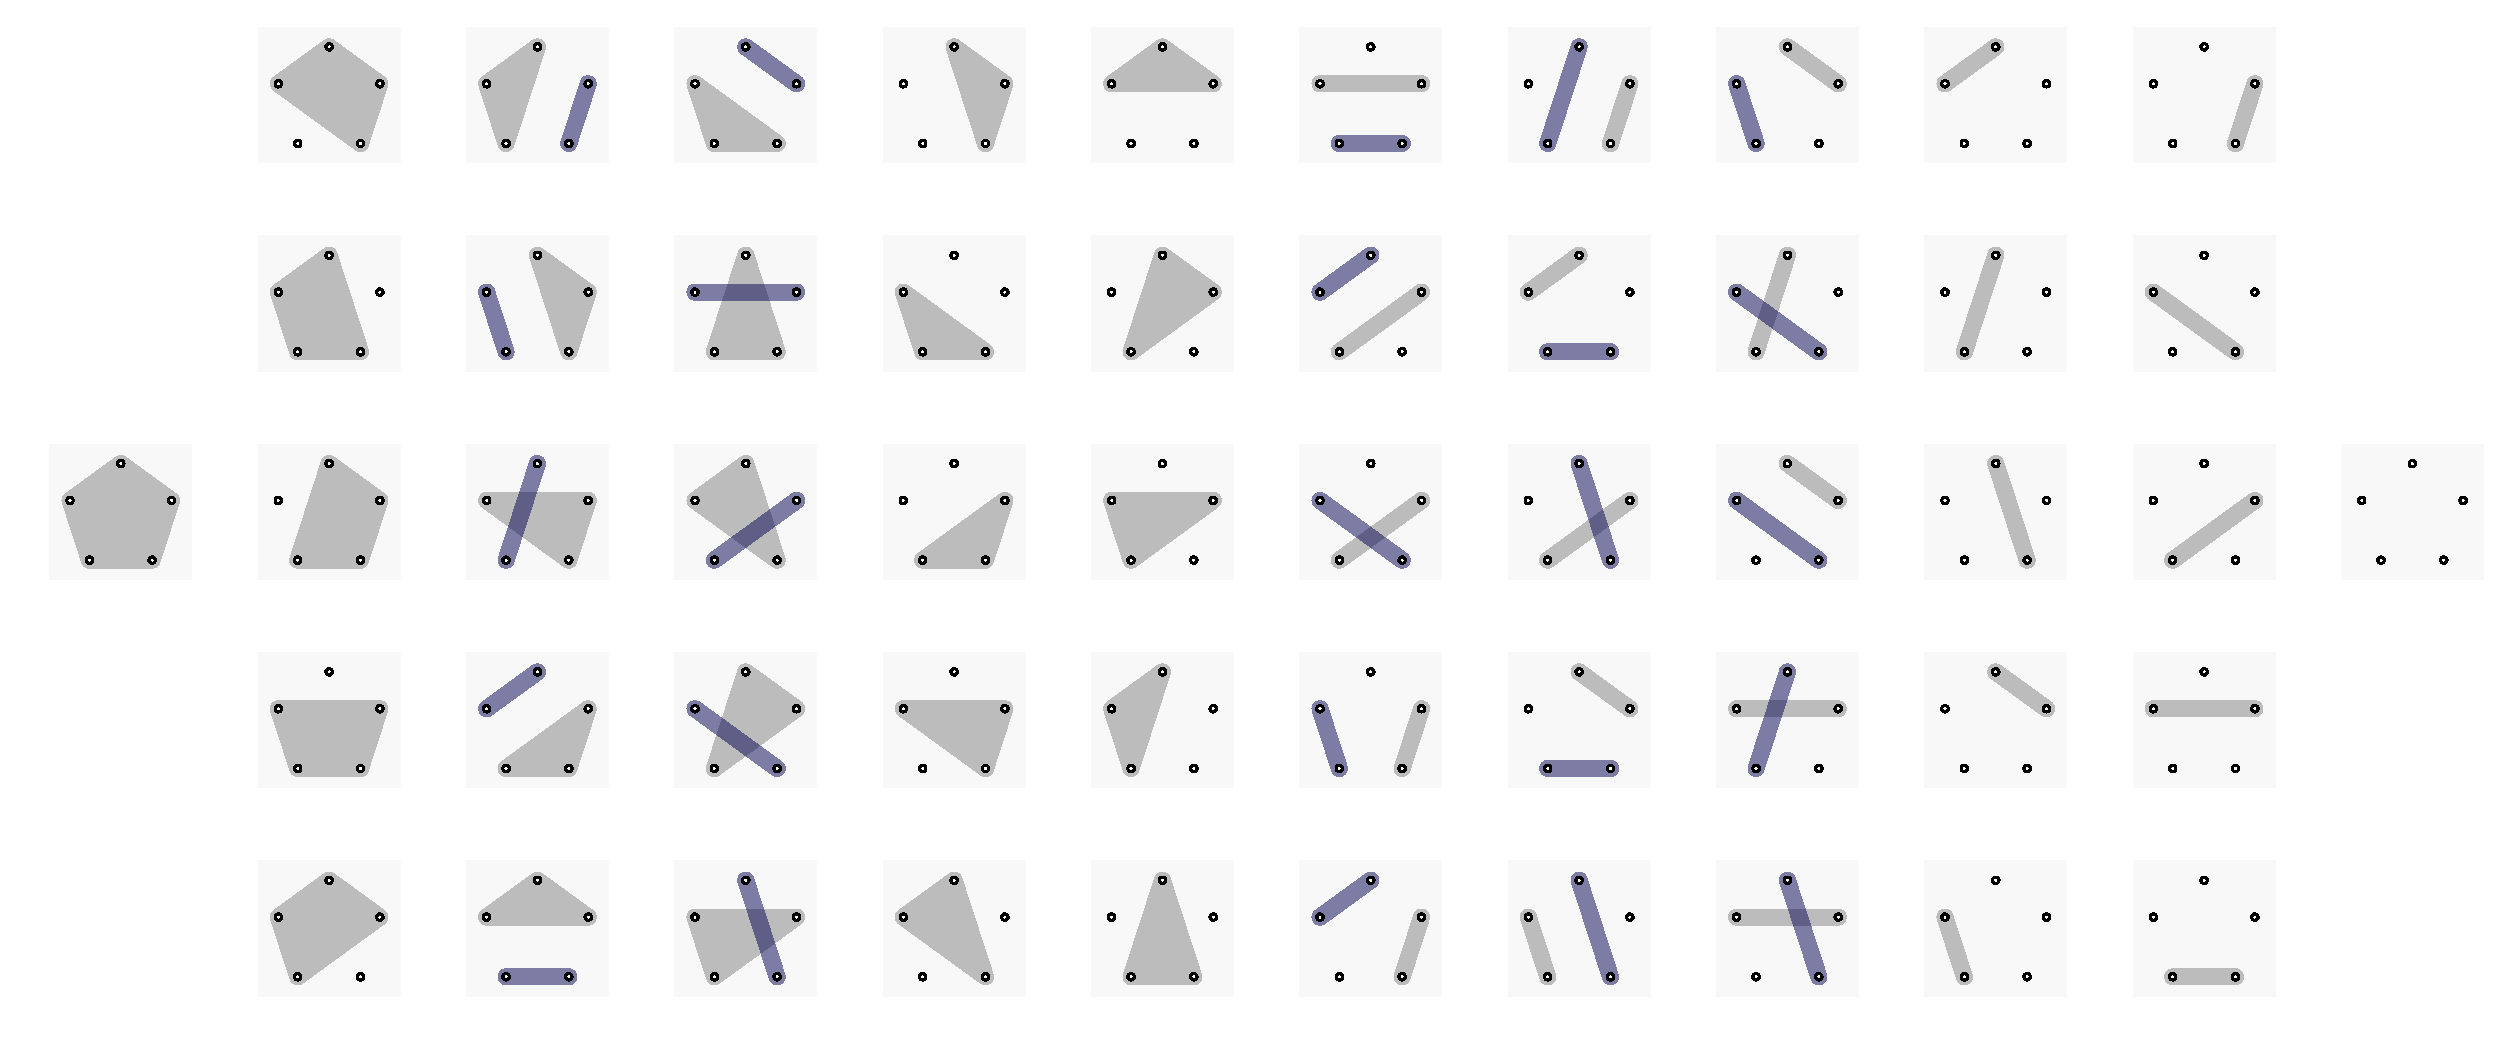
\includegraphics[width = \textwidth, keepaspectratio]{modelspace_5_horizontal.pdf}
    \caption{All 52 possible models given $K = 5$, represented as partitions. Circles represent individual parameters and shaded regions indicate which parameters are equal.}
    \label{fig:partitions}
\end{figure}

The Stirling numbers and Bell numbers can be generalized to the $r$-Stirling \parencite{broder1984r} and $r$-Bell numbers \parencite{mezo2011r}, respectively. These generalizations help to construct conditional distributions, as we will see later. The $r$-Stirling numbers $\rstirling{K}{j}{r}$ give the number of partitions of size $j$ given $K + r$ groups such that the first $r$ parameters are all in distinct subsets. The $r$-Bell numbers give the total number of partitions given $K$ parameters where the first $r$ parameters are in distinct subsets. Specifically, we have:
\begin{align}
    \rstirling{K}{j}{r} &= \sum_{i=0}^K \binom{K}{i}\stirling{i}{j}r^{K-i}\\
    \rbellnum{K}{r} &= \sum_{i=0}^K \rstirling{K+r}{i+r}{r} \enspace .
\end{align}
Note that $\rstirling{K}{j}{1} = \stirling{K}{j}$ and that $\rbellnum{K}{0} = \bellnum{K}$. Both the $r$-Stirling and $r$-Bell numbers are defined through recurrence relations, although explicit expressions exist which are easier to compute for large values; see \textcite{broder1984r} and \textcite{mezo2011r} for details.

\subsection{Urn Schemes}
We can represent the different partitions using an urn with $K$ different balls labeled 1 through $K$. For each parameter $\theta_j$, a ball $b_j$ is drawn from the urn with $b_j \in \{1, \ldots, K\}$. If two drawn balls are equal, $b_i = b_j$, then the two parameters are assigned to the same subset of the partition, that is, the two parameters $\theta_i$ and $\theta_j$ are equal if $b_i = b_j$. Note that different draws from an urn can represent the same partition. For example, the draws $(1, 1, 2)$ and $(3, 3, 1)$ both represent the partition $\{\{\theta_1, \theta_2\}, \{\theta_3\}\}$. The prior distributions introduced in the next sections assign probabilities to the unique partitions. Note that the prior probability of a particular draw can be obtained by dividing the probability of the corresponding partition by the total number of draws that correspond to that partition. The total number of draws that represent the same partition is given by $d!\binom{K}{d}$ where $d$ is the number of non-empty subsets of a particular draw.

% not sure how to bring this up
Although the urn consists of $K$ different balls, the event of interest is whether the next ball drawn equals one of the balls already drawn --- in other words, whether an equality or inequality is introduced. This event reduces the urn to a P\'{o}lya urn. All prior distributions discussed below are related to the P\'{o}lya urn. Specifically, the joint prior distribution on $(\theta_1, \ldots, \theta_K)$ is characterized by a (generalized) P\'{o}lya urn such that:
\begin{equation} \label{eq:prediction-rule}
    \theta_K \mid \theta_1, \ldots, \theta_{K - 1} \sim \begin{cases}
    \zeta_j & \text{with probability } P_{\pi} \\
    \theta_j^{\star} & \text{with probability }  1- P_{\pi} \enspace ,
    \end{cases} \numberthis
\end{equation}
where $\zeta_j$ denotes a new value for $\theta_K$ (with $\theta_1 = \zeta_1$) and $\theta_j^{\star}$ denotes a value equal to any previously observed value. We characterize the priors we discuss in the next section in terms of (\ref{eq:prediction-rule}), which is known as a \textit{prediction rule} \parencite[e.g.,][]{ishwaran2001gibbs}; in terms of the induced prior over partitions; and in terms of their penalty for multiplicity.

%\FD{\textcite{ishwaran2001gibbs} might be useful, they use Polya Urns to derive a Gibbs sampler. They say it can be used for the Dirichlet process, but also for \textit{any} prior with known \textit{prediction rule}, which is defined as $P(Y_{n+1} \mid Y_1, \ldots, Y_n)$. I think this is a useful description which allows us to distinguish between several priors (Dirichlet, Pittman-Yor, beta-binomial, etc.). Maybe note this here and then we refer to the next sections, in which we discuss the priors in slightly more detail?}
% We want to make inference over all possible partitions of some population parameter vector $\mathbf{\theta} = (\theta_1, \ldots, \theta_k)$ of size $k$. Each such partition corresponds do one particular hypothesis. The number of partitions $k$ is given by the Bell number

% \begin{equation}
%     B_{k + 1} = \sum_{i = 0}^k {k \choose i} B_k \enspace .
% \end{equation}

% The Bell numbers grow very quickly, with the number of partitions for a vector $\mathbf{\theta}$ of size 10 being 21147.


\section{Methodology} \label{sec:methodology}
Let $\vec{\theta^{\star}} = (\theta^{\star}_1, \ldots, \theta^{\star}_\len)$ denote the vector of unique population parameters out of $\vec{\theta} = (\theta_1, \ldots, \theta_K)$, $\vec{\theta}_{-j}$ the vector of parameters without parameter $\theta_j$, and the number of repeats of $\theta^{\star}_j$ as $n^{\star}_j$. Let $\rho$ denote a partition and $|\rho|$ its size. For example, if $\rho = \{\{\theta_1, \theta_2\}, \{\theta_3\}\}$, then $|\rho| = 2$. Similarly, for this example $\vec{\theta^{\star}} = (\theta^{\star}_1, \theta^{\star}_2)$ and $n^{\star} = (2, 1)$. In the next sections, we discuss and contrast a number of priors.
%\DB{I'd like to introduce $\partition_\theta$ to denote the partition of $\theta$. Any ideas?}
%\FD{Not sure I understand why — doesn't $\rho$ already denote that?}

\subsection{Dirichlet Process Prior}
The Dirichlet process (DP) is a distribution over distributions \parencite{ferguson1973bayesian}. We say that $\mathcal{G} \sim \text{DP}(\alpha, \mathcal{K})$ is distributed according to a DP if its marginal distributions are Dirichlet distributed, where $\alpha$ is a concentration parameter and $\mathcal{K}$ is the base distribution, which will depend on the application; for details, see for example \textcite{teh2010dirichlet}. The DP can be understood as the infinite-dimensional generalization of the Dirichlet distribution, which makes it popular for mixture modeling \parencite[e.g.,][]{rasmussen1999infinite}. Our modeling approach is similar to mixture modeling, except that we do not cluster data but parameters --- a cluster corresponds to a partition. The prediction rule of the DP is given by \parencite[e.g.,][]{ishwaran2001gibbs, blackwell1973ferguson}:
%Let $\vec{\theta}_{-j}$ be the vector of parameters without parameter $\theta_j$.
%\DB{I looked at these two references, and they \emph{do} define the prediction rule in an ordered way, i.e., $\theta_{n+1} \mid \theta_1,\dots,\theta_{n}$ or $\theta_{n} \mid \theta_1,\dots,\theta_{n-1}$. Perhaps we should do the same?}
\begin{equation}
    \theta_{j + 1} \mid \theta_1, \ldots, \theta_j\sim \begin{cases}
    \mathcal{K} & \text{with probability } \frac{\alpha}{\alpha + j - 1} \\
    \text{Categorical}\left(\theta_1^{\star}, \ldots, \theta_\len^{\star} \mid n^{\star}_1, \ldots, n^{\star}_\len\right) & \text{else} \enspace ,
    \end{cases} \numberthis
\end{equation}
where $\alpha$ is the concentration parameter and the base distribution of the DP depends on the application (see Section \ref{sec:applications}). In other words, we draw a new value for $\theta_j$ from $\mathcal{K}$ with probability $\nicefrac{\alpha}{\alpha + j - 1}$, or else set it to a previously observed value. The particular value $\theta^{\star}_j$ the parameter $\theta_j$ is set to is proportional to the number of times $\theta^{\star}_j$ was observed previously, given by $n^{\star}_j$, resulting in the well-known ``rich-get-richer'' property \parencite[e.g.,][]{teh2010dirichlet}.

The Dirichlet process implies a prior distribution over partitions. The prior on the partitions $\rho$ is:
\begin{equation}
    \pi(\rho \mid \alpha) = \frac{\alpha^{|\rho|}\Gamma(\alpha)}{\Gamma(n + \alpha)} \prod_{c \in \rho} \Gamma(|c|) \enspace ,
\end{equation}
where $c$ is an element of $\rho$, and $|c|$ is its size. While the Dirichlet process features the infinite-dimensional object $\mathcal{K}$, the prior over partitions results from integrating it out. Hence the nonparametric model (in which the number of parameters is not fixed) implies a parametric model (in which the number of parameters is fixed) for the partitions \parencite{quintana2006predictive}. This makes it usable for our purposes, where we have a fixed number of parameters.

The leftmost column in Figure \ref{fig:prior-comparison} shows the DP prior over partitions (top) and number of inequalities (bottom) for different values of $\alpha$. Intuitively, one reasonable requirement for a prior in the context of penalizing multiplicity is to be monotonically decreasing in the number of partitions, which further implies a monotonically decreasing prior probability over the number of inequalities. This is the case for $\alpha = 0.50$ (beige diamonds) as shown in the top and bottom panels, and indeed for any value $\alpha < 1$. The value suggested by \textcite{gopalan1998bayesian} creates a symmetric prior over the partitions (yellow suns), implying that the model with no inequalities is a priori as likely as the model with all inequalities  (in the $K = 5$ case, this yields $\alpha = 2.213$). The prior with $\alpha = 1$ (pink stars) results in a nonincreasing prior over the number of partitions, but in an increasing prior over the number of inequalities: the model with one inequality is more likely than the model with no inequalities.

%\textcolor{red}{A requirement for a prior to penalize multiplicity is to be monotonically decreasing with the number of partitions. If this were not the case, then models with many partitions, that is, many inequalities among parameters, would be assigned more prior probability than models with few partitions, that is, few inequalities among parameters.}

As $\alpha \rightarrow 0$, the prior of the model with all $K - 1$ equalities $\mathcal{M}_0$ (i.e., the null model) converges to one, while as $\alpha \rightarrow \infty$, the prior of the model with $K - 1$ inequalities $\mathcal{M}_{B_K}$ (i.e., the full model) converges to one. For prior elicitation, \textcite{gopalan1998bayesian} note that $\alpha$ is determined by specifying two of either $P(\mathcal{M}_0)$, $P(\mathcal{M}_{B_K})$, or their ratio, since $P(\mathcal{M}_0) = \nicefrac{\alpha (K - 1)!}{\prod_{j = 1}^K (\alpha + j - 1)}$ and $P(\mathcal{M}_{B_K}) = \nicefrac{\alpha^K}{\prod_{j = 1}^K (\alpha + j - 1)}$; see also Table \ref{tab:overview}.

%\textcite{escobar1995bayesian} put a Gamma prior on $\alpha$.

\begin{figure}
    \centering
    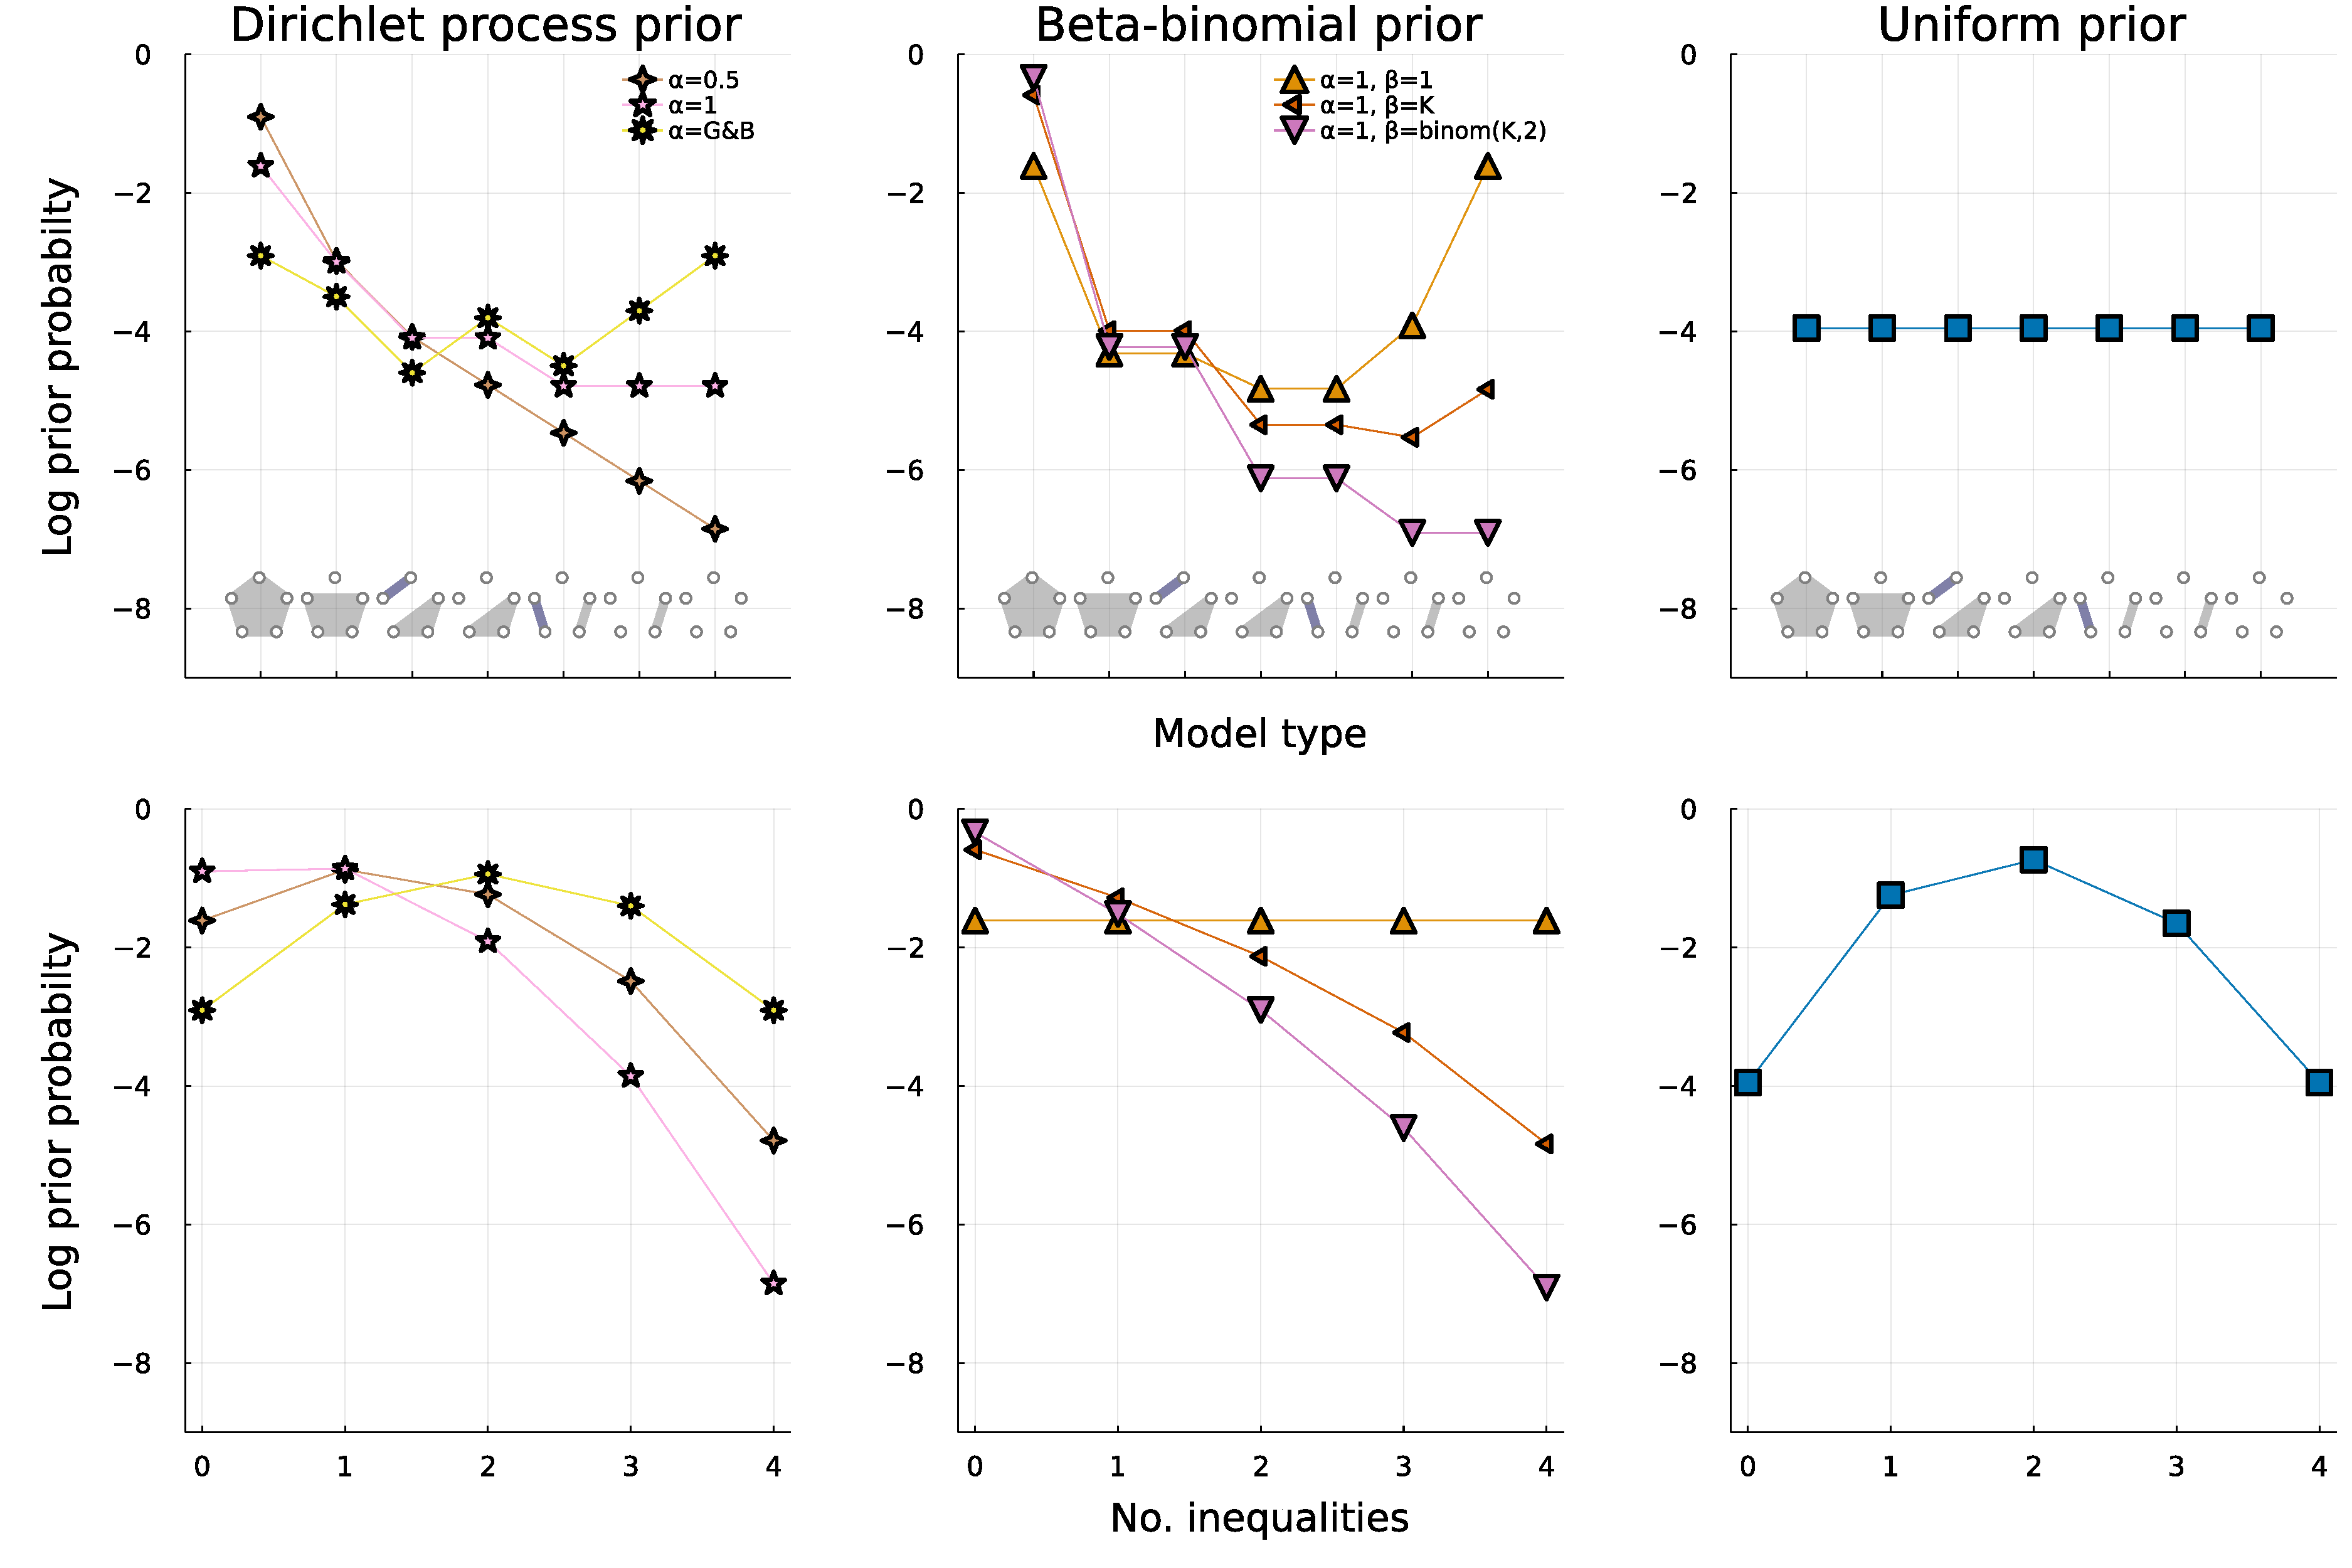
\includegraphics[width = 0.95\textwidth]{visualizePriors_2x3_new.pdf}
    \caption{Top: Dirichlet process (left), beta-binomial (middle), and uniform prior (right) across distinct model types for $K = 5$ groups and different prior parameters. Bottom: Same but for the number of inequalities across models.
    % \FD{Nice! Only thing left is to swap the order of $\beta = K$ and the binomial coefficient. If that doesn't work because it touches the line, let's not do it in this figure. I think that $\beta = K$ and $\beta = binom(K, 2)$ are incorrectly labelled and should be swapped (see also figures below).}
    } %Note that while the uniform prior is uniform over the models, it is not uniform over the number of inequalities. In contrast, the beta-binomial prior with $\alpha = \beta = 1$ is uniform over the number of inequalities but not uniform over the models.} %A key difference between the Dirichlet and beta-binomial priors is that the second and third partition, which imply the same number of equality constraints, are assigned equal prior probability by latter but not the former.}
    \label{fig:prior-comparison}
\end{figure}

\begin{table}[!htbp]
	\begin{center}
		\begingroup
		\renewcommand{\arraystretch}{1.75}
		\resizebox{\textwidth}{!}{%
			\begin{tabular}{l ccc ccc ccc}
				\toprule
				& \multicolumn{1}{c}{Dirichlet process prior} & \multicolumn{1}{c}{Beta-binomial prior} & \multicolumn{1}{c}{Uniform prior}\\
				\midrule
				Parameters  & $\alpha$ & $(\alpha = 1, \beta)$ & \xmark \\[1.4mm]
				%Prediction rule  & 8.77 & 17.09 & 31.47 \\[1.4mm]
				Prior over partitions  & $\frac{\alpha^{|\rho|}\Gamma(\alpha)}{\Gamma(n + \alpha)} \prod_{c \in \rho} \Gamma(|c|)$ & $\binom{K - 1}{|\rho| - 1}\frac{\FBeta{|\rho| - 1 + \alpha}{K - |\rho| + \beta}}{\FBeta{\alpha}{\beta}\stirling{K}{|\rho|}}$ & $\left(B_K\right)^{-1}$ \\[1.4mm]
				Prior monotonically decreasing  & $\alpha \leq 1$ & $\beta \geq K$, $\beta \geq {K \choose 2}$ & \xmark \\[1.4mm]
				Prior probability of null model  & $\nicefrac{\alpha (K - 1)!}{\prod_{j = 1}^K (\alpha + j - 1)}$ & $\nicefrac{\FBeta{\alpha}{K - 1 + \beta}}{\FBeta{\alpha}{\beta}}$ & $\left(B_K\right)^{-1}$ \\[1.4mm]
				Prior probability of full model & $\nicefrac{\alpha^K}{\prod_{j = 1}^K (\alpha + j - 1)}$ & $\nicefrac{\FBeta{K - 1 + \alpha}{\beta}}{\FBeta{\alpha}{\beta}}$ & $\left(B_K\right)^{-1}$ \\[1.4mm]
				Prior probability of ratio (null / full) & $\nicefrac{\alpha (K - 1)!}{\alpha^K}$ & $\nicefrac{\FBeta{\alpha}{K - 1 + \beta}}{\FBeta{K - 1 + \alpha}{\beta}}$ & $1$ \\[1.4mm]
				\bottomrule
		\end{tabular}}
		\endgroup
	\end{center}
	\caption{Characterizations of the different priors studied in this paper. Note: $\beta \geq K$ implies a prior decreasing in terms of the number of inequalities, but not in terms of the partitions. $\beta \geq {K \choose 2}$ implies both.}
	\label{tab:overview}
\end{table}


\subsection{Beta-binomial Prior}
%Here we briefly introduce the beta-binomial model prior, its properties, and how we can apply use it to the space of equality constraints.

The beta-binomial model prior is a popular choice for stochastic search variable selection in linear regression \parencite[][]{george1993variable} and Bayesian model averaging \parencite[e.g.,][]{hinne2020conceptual, hoeting1999bayesian}. It states that the prior probability of including $j$ predictors out of a total of $K$ predictors is given by:
\begin{equation}
    \BetaBinom{j}{K}{\alpha}{\beta} = \binom{K}{j} \frac{\FBeta{j + \alpha}{K - j + \beta}}{\FBeta{\alpha}{\beta}} \enspace ,
\end{equation}
where $\alpha$ and $\beta$ are hyperparameters. The prior probability of a particular regression model is obtained by dividing by the number of ways $j$ out of $K$ predictors can be included: $\BetaBinom{j}{K}{\alpha}{\beta} / \binom{K}{j}$. The beta-binomial distribution introduces a penalty for including additional predictors and in that way introduces a correction for multiplicity \parencite{scott2006exploration, scott2010bayes}.

\iffalse
\begin{equation}
    \pi(\rho \mid \alpha, \beta) = \binom{K}{j} \frac{\FBeta{j + \alpha}{K - j + \beta}}{\FBeta{\alpha}{\beta}} \enspace ,
\end{equation}
\fi

% Fabian: This was the equation we had before, which is incorrect
%\begin{equation}
%    \pi(\rho \mid K, \alpha, \beta) = \binom{K - 1}{|\rho| - 1}
%    \frac{\FBeta{|\rho| - 1 + \alpha}{K - |\rho| - 2 + \beta}}
%    {\FBeta{\alpha}{\beta}\stirling{K-1}{K-|\rho|-1}} \enspace ,
%\end{equation}

For the multiple comparison problem discussed in this paper, we consider the number of inequality constraints and use the beta-binomial prior to introduce a penalty for each additional inequality among the groups considered. For $K$ groups, there can be a maximum of $K - 1$ inequalities, resulting in a $\BetaBinom{i}{K-1}{\alpha}{\beta}$ prior distribution over the number of included inequalities $i$ out of $K$ groups. To see how this translates to a prior over the partitions $\rho$, note that there is a one-to-many correspondence between the number of inequalities $i$ out of $K$ groups and the resulting partitions $\rho$. For example, having $i = 1$ inequalities with $K = 3$ groups is consistent with the partitions $\{\{\theta_1, \theta_2\}, \{\theta_3\}\}$, $\{\{\theta_1, \theta_3\}, \{\theta_1\}\}$, and $\{\{\theta_2, \theta_3\}, \{\theta_1\}\}$, all of which are of size $|\rho| = i + 1$. The number of partitions of size $|\rho|$ is given, as discussed above, by the Stirling number $\stirling{K}{|\rho|}$. For the assignment of the prior probability, it is only the size of the partition (the number of inequalities) that counts. With these observations in hand, we arrive at the following (adjusted) beta-binomial prior distribution over partitions $\rho$:
\begin{equation}
    \pi(\rho \mid K, \alpha, \beta) = \binom{K - 1}{|\rho| - 1}
    \frac{\FBeta{|\rho| - 1 + \alpha}{K - |\rho| + \beta}}
    {\FBeta{\alpha}{\beta}\stirling{K}{|\rho|}} \enspace .
\end{equation}
The prediction rule of the beta-binomial prior is given by:
\begin{equation}
    \theta_{j + 1} \mid \theta_1, \ldots, \theta_j \sim \begin{cases}
    \mathcal{K} & \text{with probability } P_{\pi} \\
    \text{Categorical}\left(\theta_1^{\star}, \ldots, \theta_\len^{\star} \mid 1, \ldots, 1\right) & \text{else} \enspace .
    \end{cases} \enspace , \numberthis
\end{equation}
where
\begin{align}
    P_{\pi} &=
    \frac{
        % \sum_{\substack{\partition \in \Rho\\\vec{\theta} \subseteq \rho\\\theta_j \notin \vec{\theta}_{-j}}}
        \sum_{\substack{\partition \in \Rho\\\theta_j \notin \vec{\theta}_{-j} \subseteq \rho}}
        \BetaBinom{\rho}{K}{\alpha}{\beta}
    }{
        % \sum_{\substack{\partition \in \Rho\\\vec{\theta} \subseteq \rho\\\theta_j \notin \vec{\theta}_{-j}}}
        \sum_{\substack{\partition \in \Rho\\\theta_j \notin \vec{\theta}_{-j} \subseteq \rho}}
        \BetaBinom{\rho}{K}{\alpha}{\beta} +
        % \sum_{\substack{\partition \in \Rho\\\vec{\theta} \subseteq \rho\\\theta_j \in \vec{\theta}_{-j}}}
        \sum_{\substack{\partition \in \Rho\\\theta_j \in \vec{\theta}_{-j} \subseteq \rho}}
        \BetaBinom{\rho}{K}{\alpha}{\beta}\label{eq:11}
    } \enspace ,
\intertext{and where $\Rho$ denotes the set of all possible partitions. In essence, Equation \eqref{eq:11} takes the probability of all possible partitions where $\theta_j$ is distinct from $\vec{\theta}_{-j}$, conditional on $\vec{\theta}_{-j}$ being a subset of the considered partition. The sum over all possible partitions can be simplified using the $r$-Stirling numbers:}
    P_{\pi} &=
    \frac{
        \sum_{i=1}^K \BetaBinom{i}{K}{\alpha}{\beta} \rstirling{K-j+\len+1}{i}{\len + 1}
    }{
        \len \sum_{j=i}^K \BetaBinom{i}{K}{\alpha}{\beta} \rstirling{K-j+\len}{i}{\len} +
             \sum_{i=1}^K \BetaBinom{i}{K}{\alpha}{\beta} \rstirling{K-j+\len+1}{i}{\len + 1}
    } \enspace ,
\end{align}
where $\len$ is number of unique parameters in $\vec{\theta}$, that is, the size of the partition.
% \DB{The paragraph below makes no sense.}
% where $s_j = \setsize{\{\theta_1, \ldots, \theta_{j - 1}\}}$ is the number of distinct elements in $\{\theta_1, \ldots, \theta_{j - 1}\}$. The $r$-Stirling number in the numerator counts the number of models with $i$ equalities if $\theta_j$ is a new value. Next, this is multiplied by the probability of including $i$ equalities. This is summed for all possible numbers of equalities.
% The first sum in the denominator does the same, assuming that $\theta_j$ is a value in $\{\theta_1, \dots, \theta_{j-1}\}$. With probability $1 - P_{\pi}$ we have that $\theta_j$ is equal to one of the previously drawn parameters. This draw is from a categorical distribution over the possible models, that is, conditional on drawing a previous value the probability of $\theta_j = \theta_i$ is proportional to $\rbellnum{K-i-1}{s_j}$. \FD{Double check this and adjust the text and Equation (9). Make clear that this is exchangeable; do Equation (10) and show that this yields the beta-binomial.}

The beta-binomial prior on the partitions and the induced prior on the number of inequalities are shown for different parameterizations in the middle column in Figure \ref{fig:prior-comparison}. For $\alpha = \beta = 1$, the beta-binomial distribution over the partitions has a characteristic U-shape (orange triangles). This prior specification in turn implies a uniform prior on the number of inequalities. We follow \textcite{wilson2010bayesian} who, in the context of regression, suggested to set $\alpha = 1$ as a default so that the distribution over model size (here the number of inequalities) is nonincreasing, and to scale $\beta = \lambda K$ with the number of groups to force the prior to be monotonically decreasing, with a default of $\lambda = 1$ \parencite{wilson2010bayesian}. This is illustrated as the red line (leftward pointing triangles) in Figure \ref{fig:prior-comparison} using $\beta = 5$. In the multiple comparison case, we additionally investigate $\beta = {K \choose 2}$, which implies that the prior on the number of inequalities of individual models is nonincreasing, see Appendix~\ref{ap:decreasing-odds}. The purple line (upside-down triangles) in Figure \ref{fig:prior-comparison} shows a decreasing prior for $\beta = {5 \choose 2} = 10$. This prior assigns the least mass to models with an increasing number of inequalities compared to all others beta-binomial priors.
% \DB{1. I'm not sure if ``... and no penalty for multiplicity.'' is entirely correct. 2. We need to tone down}

% The difference is that in our prior specification the roles of $\alpha$ and $\beta$ are reversed.

Figure \ref{fig:prior-comparison} shows that the DP prior makes a distinction that the beta-binomial is, by design, not making: while the beta-binomial prior assigns the same prior mass to partitions with the same number of (in)equalities, the DP prior assigns more mass to the partition with the larger cluster. For example, the beta-binomial does not distinguish between $\{\{\theta_1, \theta_2, \theta_3\}, \{\theta_4\}, \{\theta_5\}\}$ and $\{\{\theta_1, \theta_2\}, \{\theta_3, \theta_4\}, \{\theta_5\}\}$, while the DP assigns more mass to the former (see Figure \ref{fig:prior-comparison}). We return to this distinction in the discussion.

Lastly, note that for the beta-binomial prior we have that $P(\mathcal{M}_0) = \nicefrac{\FBeta{\alpha}{K - 1 + \beta}}{\FBeta{\alpha}{\beta}}$ and $P(\mathcal{M}_{B_K}) = \nicefrac{\FBeta{K - 1 + \alpha}{\beta}}{\FBeta{\alpha}{\beta}}$. Fixing $\alpha = 1$, we have that as $\beta \rightarrow \infty$, the prior of the model with all $K - 1$ equalities $\mathcal{M}_0$ converges to one, while as $\beta \rightarrow 0$, the prior of the model with $K - 1$ inequalities $\mathcal{M}_{B_K}$ converges to one; see also Table \ref{tab:overview}. As with the Dirichlet process prior discussed above, one can use these relations in prior elicitation.


\subsection{Uniform Prior}
%\FD{The paper by \textcite{wallach2010alternative} seems extremely relevant here. The define the uniform process as having a prediction rule that is uniform over the already existing partitions ... so not quite the same. How is it related to what we do here? Actually, they show that the expected number of clusters of size $M$ is a constant, so it seems to be exactly what we do. Interestingly, the uniform process is not exchangeable. Also, it seems to me that it will not penalize multiplicity.}
For completeness, we give a prior that is uniform over the space of partitions. The probability mass function is straightforward. All valid configurations of size $K$ have probability $\nicefrac{1}{\bellnum{K}}$. The prediction rule of the uniform prior is given by:
\begin{equation}
    \theta_{j + 1} \mid \theta_1, \ldots, \theta_j%, \ldots, \theta_{j - 1}, \theta_{j + 1}, \ldots, \theta_{K}
    \sim \begin{cases}
    % \mathcal{K} & \text{with probability } \rbellnum{K - j - 1}{s_j + 1} \\
    % \text{Categorical}\left(\theta_1^{\star}, \ldots, \theta_\len^{\star} \mid \rbellnum{K - 1 - 1}{s_1}, \ldots, \rbellnum{K - m - 1}{s_\len}\right) & \text{else} \enspace ,
    \mathcal{K} & \text{with probability } P_{\pi_{U}} \\
    \text{Categorical}\left(\theta_1^{\star}, \ldots, \theta_\len^{\star} \mid 1, \ldots, 1\right) & \text{else} \enspace ,
    \end{cases} \numberthis
\end{equation}
where
\begin{align}
    P_{\pi_{U}} %&=
    % \frac{\text{(\# partitions with size $\len + 1$)}}{\text{(\# partitions with size $\len + 1$)} + (\len \times \text{\# partitions with size $\len$)}}\\[0.50em]
    &=
    \frac{\rbellnum{K-j+1}{\len + 1}}{\rbellnum{K-j+1}{\len + 1} + \len\rbellnum{K-j+1}{\len}}
\end{align}
Here, $\rbellnum{K-j+1}{\len + 1}$ counts the number of models where $\theta_{j+1} \notin \left(\theta_1^{\star}, \ldots, \theta_\len^{\star}\right)$ conditional on $\theta_1, \ldots, \theta_j$ being assigned to $\len$ distinct subsets.
Complementarily, $\rbellnum{K-j+1}{\len}$ counts the number of models where $\theta_{j+1} \in \left(\theta_1^{\star}, \ldots, \theta_\len^{\star}\right)$ conditional on $\theta_1, \ldots, \theta_j$ being assigned to $\len$ distinct subsets, which is multiplied by $\len$ as there are $\len$ subsets that $\theta_{j+1}$ could be assigned to. Under this uniform prior, all partitions $\rho$ are equally likely, as can be seen in the top right panel in Figure \ref{fig:prior-comparison}. Note that this uniform prior induces a non-uniform prior on the number of inequalities, as shown in the bottom right panel.
% \FD{The paragraph below is not super clear, let's sharpen this.}
% For the first value $\theta_1$, the drawn value is irrelevant as it does not introduce an (in)equality. For the second draw we consider two cases. First, the probability of drawing a new value $\theta_2 \neq \theta_1$ is proportional to the number of partitions where the first two elements are in distinct subsets, which is given by $\rbellnum{K - 2}{2}$. The probability of sampling a particular new value is uniformly divided over the possible labels; hence to obtain the probability for a particular new value we divide by $K - s_j$. \FD{I don't understand the previous sentence, let's discuss.} Second, the probability of drawing an old label, $\theta_2 = \theta_1$, is proportional to the number of partitions where the first element is in a distinct subset. Under this uniform prior, all partitions $\rho$ are equally likely, as can be seen in the top right panel in Figure \ref{fig:prior-comparison}. Note that this uniform prior induces a non-uniform prior on the number of inequalities, as shown in the bottom right panel.

\iffalse
\begin{equation}
    \prior{\theta_i \mid \theta_1, \ldots, \theta_{i - 1}} = \begin{cases}
    \zeta_i & \text{with probability proportional to } \rbellnum{k - i - 1}{s_i + 1} \\
    \theta_i^\ast & \text{with probability proportional to }  \rbellnum{k - i - 1}{s_i} \enspace
    \end{cases} \numberthis
\end{equation}
\fi

\subsection{Posterior Model Consistency}
Model selection consistency is a key desiderata that a good Bayes factor should fulfill \parencite[e.g.,][]{bayarri2012criteria, ly2016harold, consonni2018prior}. In the situation of multiple models, the notion of pairwise model selection consistency needs to be extended. This extension is referred to as posterior model selection consistency. Posterior model consistency in a model class $\mathfrak{M}$ is the convergence to one, in probability, of the posterior probabilities to the true model \parencite[e.g.,][]{casella2009consistency, moreno2015posterior}. Let $\mathcal{M}_j \in \mathfrak{M}$ be the model that instantiates the hypothesis $\mathcal{H}_j$ that specifies the (in)equalities among $K$ groups. The posterior probability of $\mathcal{M}_j$ is given by:
\begin{align}
    p(\mathcal{M}_j \mid \mathcal{D}) &= \frac{p(\mathcal{D} \mid \mathcal{M}_j) \pi(\mathcal{M}_j)}{\sum_{i = 0}^{\bellnum{K}} p(\mathcal{D} \mid \mathcal{M}_i) \pi(\mathcal{M}_i)}
    = \frac{\text{BF}_{j0}\pi(\mathcal{M}_j)}{\sum_{i = 0}^{\bellnum{K}} \text{BF}_{i0} \pi(\mathcal{M}_i)} \enspace .
\end{align}
It follows that if the Bayes factor is model selection consistent, posterior model consistency holds \parencite[see also][Theorem 1]{moreno2015posterior} --- unless the prior assigns zero mass to the true model. This is not the case for any of the priors discussed above, and hence whether posterior model consistency holds depends solely on the priors on the parameters within models.

\subsection{Stochastic Search Method} \label{sec:method-description}
When the number of groups is small and the computation of Bayes factors is swift, one can directly compute the Bayes factors for all hypotheses. Using the priors we outlined above, one can then obtain posterior distributions over hypotheses that incorporate the desired multiplicity adjustment. The number of (in)equalities grows extremely quickly with the number of groups, however, and for larger number of groups one must rely on stochastic search methods. Moreover, while directly computing the Bayes factors results in posterior distributions over hypotheses, it does not yield posterior distributions over parameters. We therefore set up a stochastic search method that yields both, allowing researchers to incorporate uncertainty across hypotheses through model averaging \parencite[e.g.,][]{hinne2020conceptual, hoeting1999bayesian}.

Our method is implemented in the programming language Julia \parencite{Julia2017Bezanson}. First, we implemented the prior distributions in Julia. Next, we used the library \emph{Turing.jl}, which is designed for general-purpose probabilistic programming \parencite{Turing2018Ge}. Turing enabled us to directly reuse the distributions defined in Julia code and also provided a multitude of options for composing different MCMC samplers. We set up a Gibbs sampler that explored the posterior space in two steps. The first step used Turing's built-in Hamiltonian Monte Carlo methods for sampling from the posterior distributions of the continuous parameters. In all models discussed here, all parameters are continuous except for the partitions. The second step used a custom Gibbs algorithm for sampling from the posterior distribution over partitions. The partitions were represented as a vector of integers denoted $\vec{\gamma}$ that indicate partition membership. By partition membership, we mean that two parameters $\theta_i$ and $\theta_j$ are in the same partition if and only if $\gamma_i = \gamma_j$. For example, $\{\{\theta_1\}, \{\theta_2, \theta_3\}\}$ could be represented by $(1, 2, 2)$ but also by $(3, 1, 1)$. We first explain the remainder of the sampling scheme and motivate the duplicate representations in the next paragraph. The number of possible duplicate representations in $\vec{\gamma}$ for one partition is straightforward to compute, and the prior over $\vec{\gamma}$ is obtained by taking the prior over the partitions and dividing uniformly over duplicate representations. Next, we sample each element of $\vec{\gamma}$ conditional on the other elements. Since the partition membership is discrete, we enumerate all possible values and draw from the resulting categorical distribution. Sampling individual elements of $\vec{\gamma}$ from the conditional distributions rather than the joint distribution reduces the complexity from $\mathcal{O}(B_K)$ to $\mathcal{O}(K^2)$.

Although the duplicate representations of $\vec{\gamma}$ for one partition introduce some additional computational cost, they facilitate exploration of the posterior space. For example, if we had used a one-to-one mapping from partitions to $\vec{\gamma}$, then updating the first membership in $(1, 2, 2)$ to $(2, 2, 2)$ would not be a valid configuration, as this should be represented by $(1, 1, 1)$. However, a transition from $(1, 2, 2)$ to $(1, 1, 1)$ requires updating two parameters and is therefore less likely to occur. Nevertheless, on the level of partitions, it makes sense to propose a move from $\{\{\theta_1\}, \{\theta_2, \theta_3\}\}$ to $\{\{\theta_1, \theta_2, \theta_3\}\}$.


\section{Investigating Multiplicity Adjustment} \label{sec:simulation-study}
In this section, we investigate the differences between the above priors in more detail and compare them to the method proposed by \textcite{westfall1997bayesian} and an uncorrected approach using pairwise Bayes factors. In Section \ref{sec:illustration}, we use a small simulation study to illustrate the implications of multiplicity adjustment. In Section \ref{sec:simulation}, we present the results of a more extensive simulation study.

%In Section \ref{sec:scott-berger}, we use a visualization inspired by \textcite{scott2010bayes} to illustrate the extent to which different priors penalize multiplicity.

\subsection{Illustrating Multiplicity Adjustment} \label{sec:illustration}
Here we illustrate the different multiplicity penalties that the different priors impose using a small simulation study. We simulate data from a one-way ANOVA model and analyze it using the specification by \textcite{rouder2012default}. The ANOVA model extended with a prior over partitions is given by:
\begin{align*}
    Y_{ij}              &\sim \mathcal{N}\left(\mu + \sigma\theta_j, 1\right)\\
    \mu                 &\propto 1  \\
    \sigma^2            &\propto 1 / \sigma^2 \\
    g                   &\sim \mathcal{IG}\left(\nicefrac{1}{2}, \nicefrac{1}{2}\right) \\
    \vec{\theta}^u   &\sim \mathcal{N}_{K-1}\left(0, g\right)   \\
    \vec{\theta}^c   &\leftarrow \mathbf{Q}\vec{\theta}^u \\
    \theta_j            &\leftarrow \text{mean of elements of } \theta^c \text{ in the same partition }\\
    \rho                &\sim \pi_{\rho}(.) \enspace . \numberthis
\end{align*}
The data follow a Gaussian distribution with a grand mean $\mu$ and a group-specific offset $\theta_j$. The offsets sum to zero to avoid identification constraints. This is achieved by projecting $\vec{\theta}^u$ from a $K-1$ dimensional space onto a $K$ dimensional space using the matrix $\mathbf{Q}$, which consists of the first $K-1$ columns of an eigendecomposition of a degenerate covariance matrix as defined in \textcite{rouder2012default}.\footnote{Note that this projection is not unique. It can also be achieved with, for example, a QR decomposition, as recommended by the \textcite{stanUserManual}.} Next, the elements of $\vec{\theta}^c$ within the same partition are averaged to obtain $\theta_j$. The unconstrained offsets $\vec{\theta}^u$ are assigned a $g$ prior where $g$ itself is assigned an inverse gamma prior with shape and scale equal to \nicefrac{1}{2} \parencite{liang2008mixtures}. Note that the model reduces to the approach of \textcite{rouder2012default} whenever the partition indicates that all elements are distinct.

%\FD{Changing $\alpha$ scales bottom row in Figure 3 – describe this! Top BB is models, not model classes (that's why it's not monotonically decreasing)}

We simulated from the null model, which assumes that all the groups are equal, and from the full model, which assumes that all groups are unequal, drawing 100 observations per group and varying the number of groups $K \in [2, 3, \dots, 10]$, repeating each combination 100 times. In the full model, the means were of increasing size with successive differences of $0.20$. For the analysis we considered six priors: the Dirichlet process prior with $\alpha \in \{0.50, 1\}$ and $\alpha$ set adaptively to have equal prior mass assigned to the model with all equalities and the model with all inequalities (i.e., $p(\mathcal{H}_0) = p(\mathcal{H}_1)$), as done by \textcite{gopalan1998bayesian}; the beta-binomial prior with $\alpha = 1$ and $\beta \in \{1, K, {K \choose 2}\}$; and the uniform prior. We also included the prior adjustment method proposed by \textcite{westfall1997bayesian} and an uncorrected method using pairwise Bayes factors. We used our methodology as described in Section \ref{sec:method-description}, drawing 12,000 MCMC samples and discarding the first 2,000 as a burn-in.

To assess how well the respective priors adjust for multiplicity, we calculated how frequently the posterior probability that any two groups differ is larger than 0.50, using the null model as data-generating model. Similarly, to assess how well the respective priors are capable of detecting true differences, we calculated how frequently the posterior probability that any two groups \textit{do not} differ is larger than 0.50, using the full model as data-generating model.

\begin{figure}
    \centering
    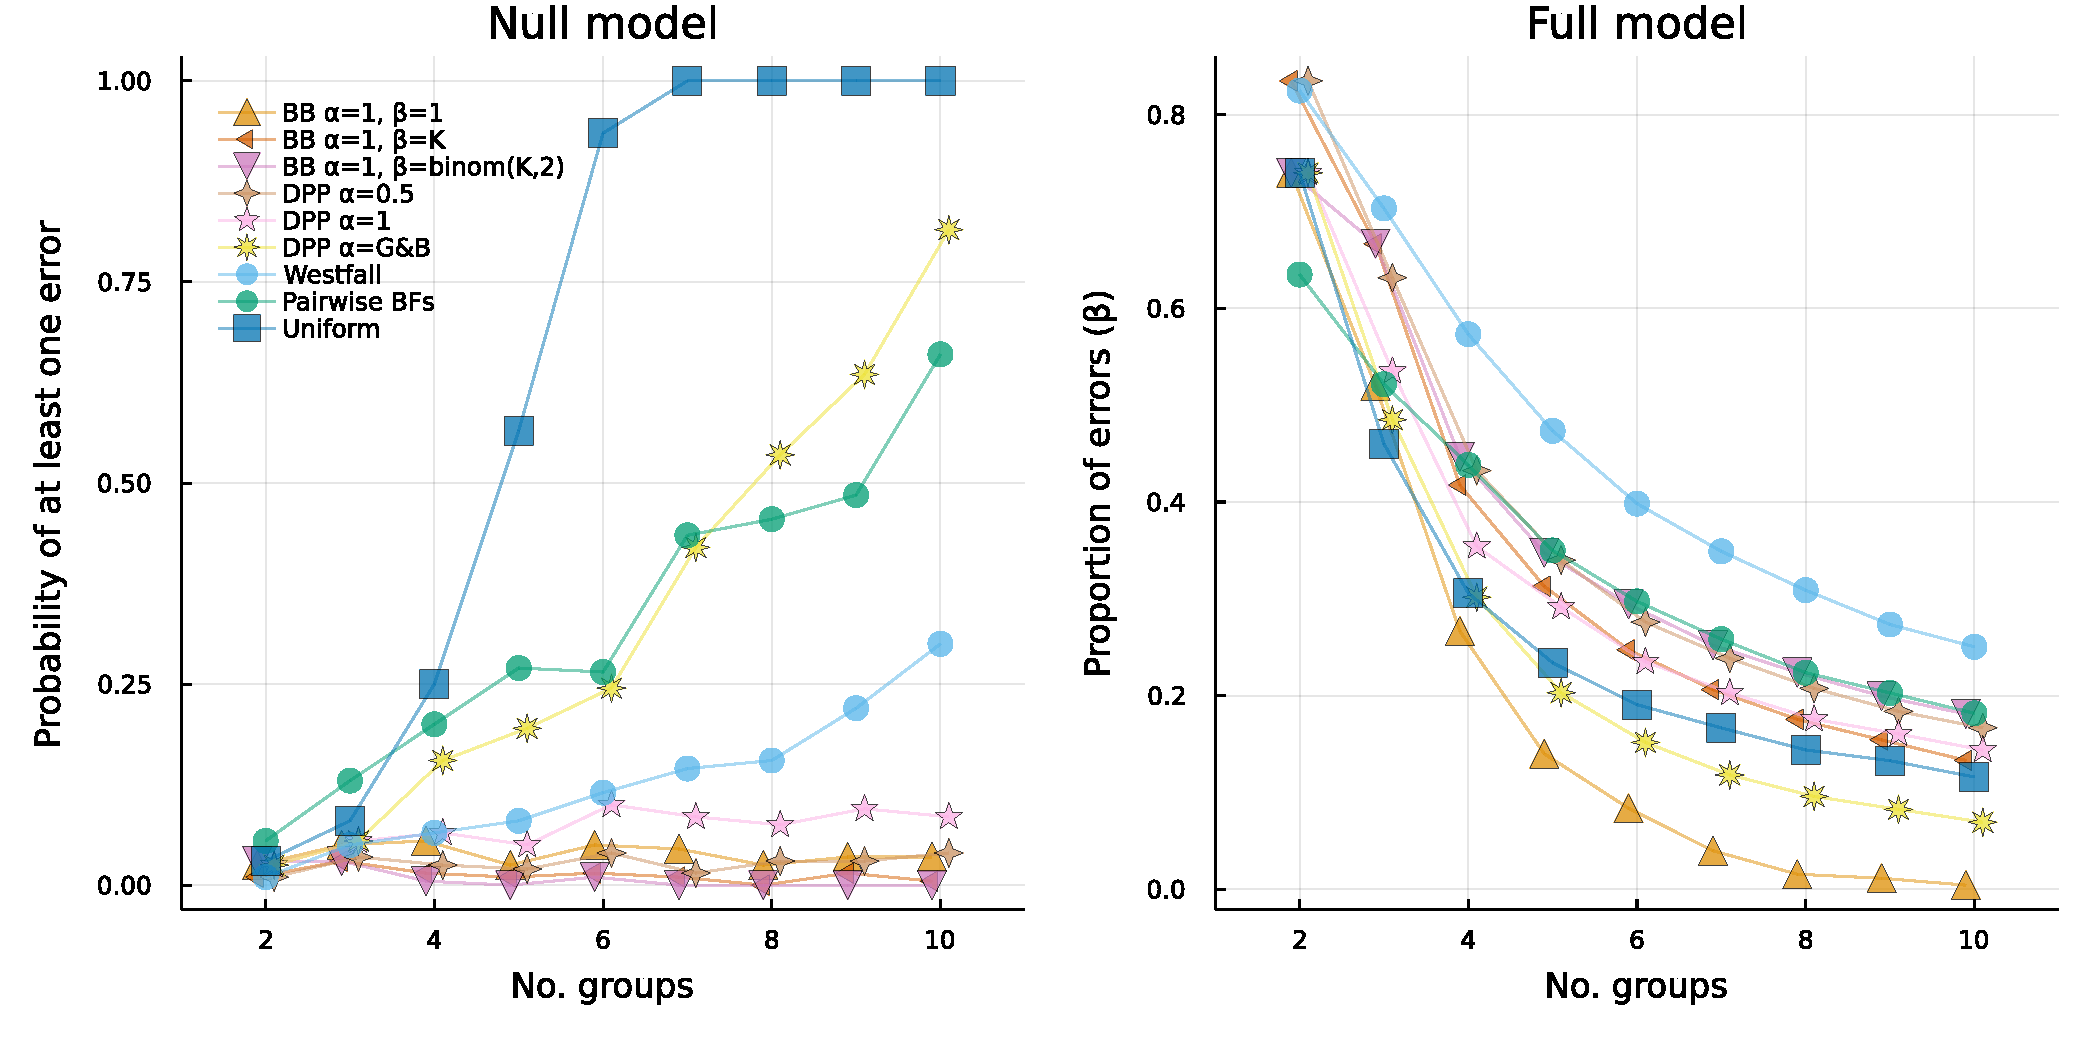
\includegraphics[width=1\textwidth]{2_panel_alpha_familywise.pdf}
    \caption{Left: Probability of making at least one false claim about a difference between two groups when there is none. Right: Proportion of falsely claiming no difference between two groups when there is one. %All measures as a function of the number of groups $K$ for different priors; see main text for details.
    % \FD{Can we swap the order of $\beta = K$ and the binomial coefficient? Same in Figure 4.}
    }
    \label{fig:small_simulation}
\end{figure}

\iffalse
\begin{figure}
    \centering
    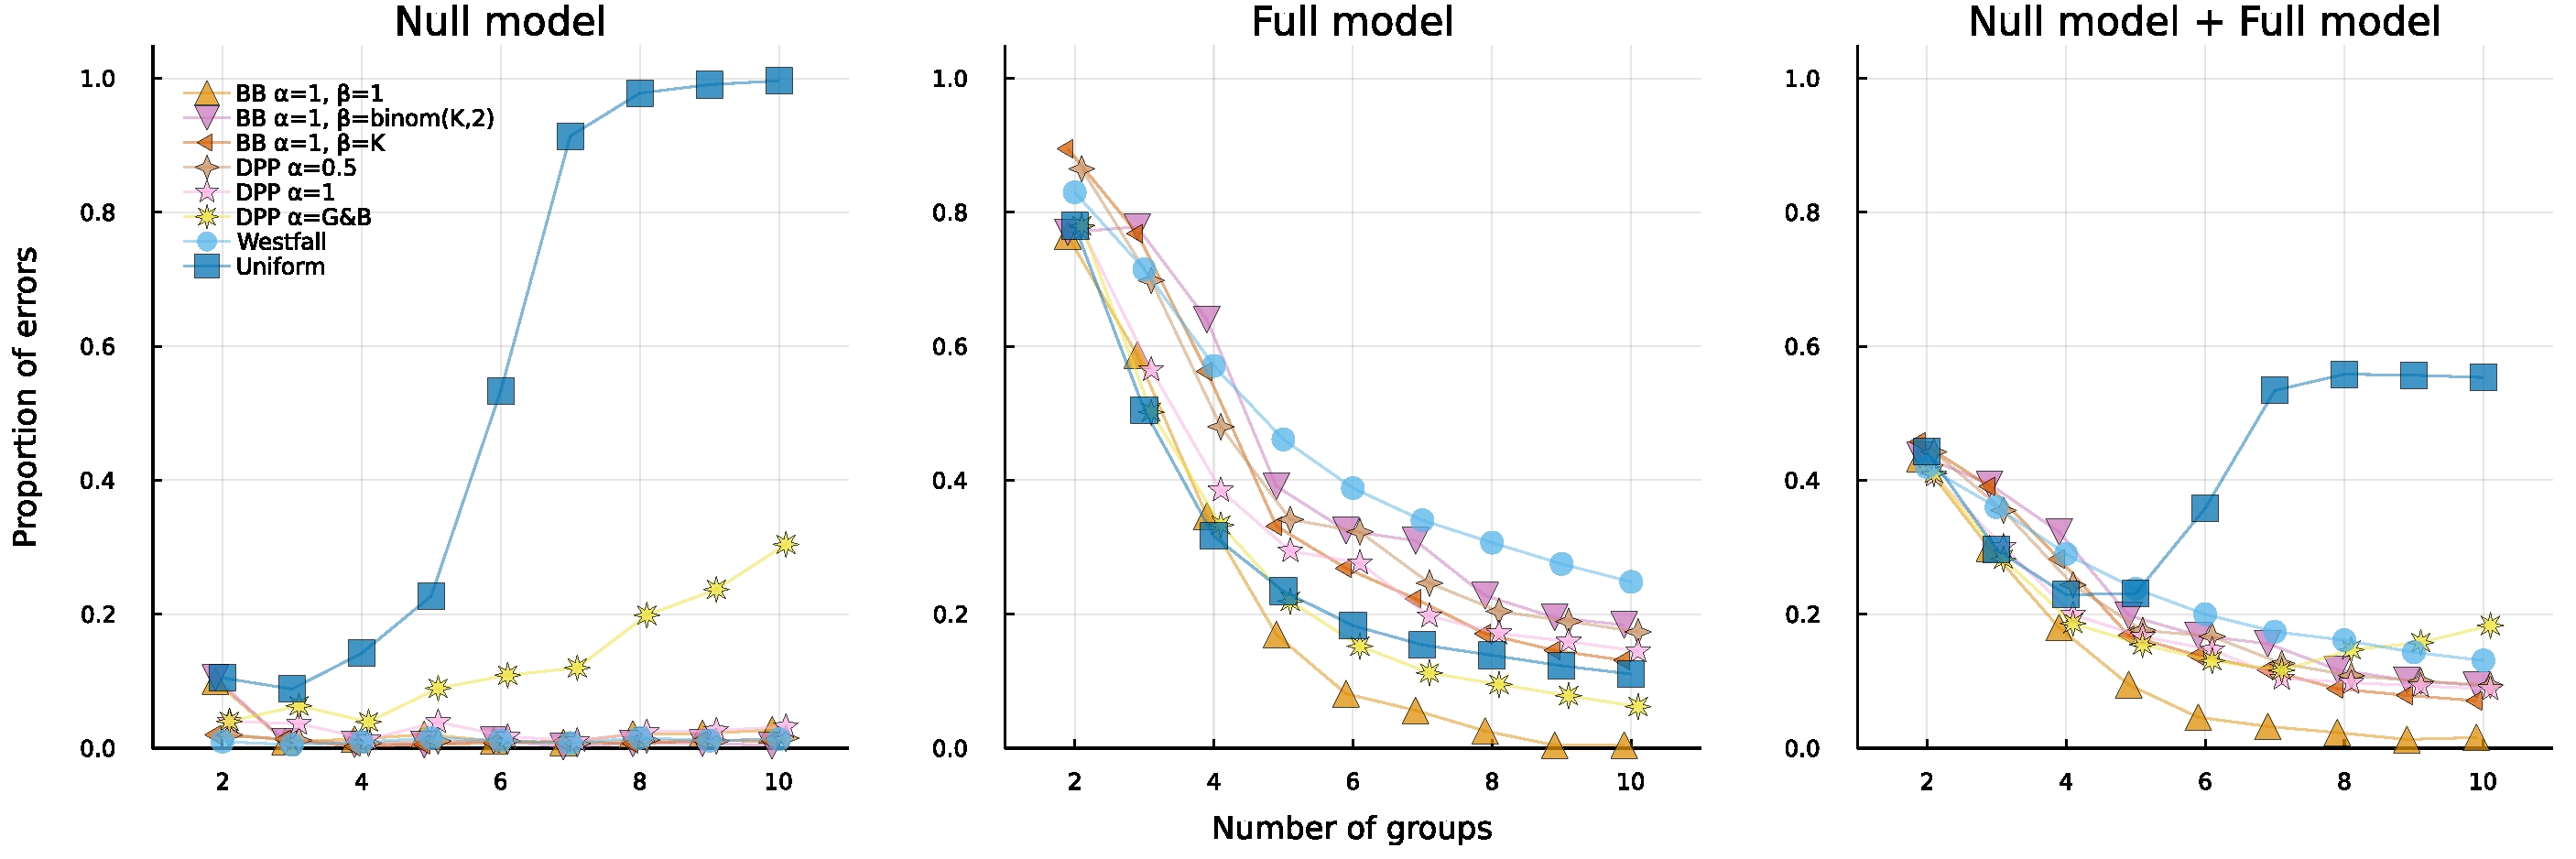
\includegraphics[width=1\textwidth]{multipleComparisonPlot_lambda_4x4_2.pdf}
    \caption{Left: Probability of at least once falsely claiming a difference between two groups when there is none under the null model. Right: Proportion of falsely claiming no difference between two groups when there is one under the full model. All measures are a function of the number of groups $K$ for different priors; see main text for details.}
    \label{fig:small_simulation}
\end{figure}
\fi


The left panel in Figure~\ref{fig:small_simulation} shows that using a uniform prior (blue squares) very quickly leads to false positives as the number of groups increases. This is not surprising: the uniform prior assigns each model the same prior mass, hence diminishing the plausibility assigned to $\mathcal{H}_0$ dramatically as $K$ increases, thus increasing the probability of an error. The Dirichlet process prior which assigns equal mass to the full and the null model (yellow suns), as suggested by \textcite{gopalan1998bayesian}, performs better than the uniform prior but still does not provide adequate error control. It performs roughly as poorly as the method which simply computes pairwise Bayesian $t$-tests (green circles). The correction proposed by \textcite{westfall1997bayesian} performs much better (light blue circles) but still leads to a relatively high probability of making at least one error as the number of groups increases. The DP prior with $\alpha = 1$ (pink stars) performs better, with the DP prior with $\alpha = 0.50$ (beige diamonds) and the set of beta-binomial priors providing good error control.

The right panel in Figure~\ref{fig:small_simulation} shows that the beta-binomial prior with $\alpha = \beta = 1$ leads to the lowest proportion of falsely claiming no difference between two groups, followed by the Dirichlet process prior for which $p(\mathcal{H}_0) = p(\mathcal{H}_1)$ and the uniform prior. The method proposed by \textcite{westfall1997bayesian} performs worst, followed by the beta-binomial prior with $\alpha = 1$ and $\beta = {K \choose 2}$ and the DP prior with $\alpha = 0.50$. The performance of the uncorrected pairwise Bayes factor approach is somewhere in the middle. Note that all approaches perform better as the group size increases, but this is due to our simulation design: each additional group exhibits a mean larger than the previous one by $0.20$ and adds $n$ more observations, which makes falsely claiming no difference less likely with an increasing number of groups. Instead of looking at absolute error, we therefore focus on the relative ordering of the priors. Overall, we conclude that not adjusting for multiple comparisons — either by using a uniform prior or by using pairwise Bayes factors — naturally leads to the worst performance and that the method by \textcite{westfall1997bayesian} is overly conservative and does not provide adequate error control with an increasing number of groups. In the next section, we report on a more extensive simulation study to further disentangle the differences between the multiple comparison methods.


%The right panel in Figure~\ref{fig:small_simulation} gives equal weight to both types of errors and combines them into a single measure. This shows that the beta-binomial prior with $\alpha = \beta = 1$ performs best. This is not so surprising, because this prior assigns both the null and the full model the highest prior probability, thereby mimicking the simulation setup most closely. While the parameterization of the Dirichlet process as proposed by \textcite{gopalan1998bayesian} does this as well, it assigns more combined prior mass to models with at least some inequalities, as shown in the bottom left panel in Figure \ref{fig:prior-comparison}. The uniform prior results in a similar distribution over the number of included inequalities, as shown in the bottom panel in Figure \ref{fig:prior-comparison}. The beta-binomial prior, on the other hand, results in a uniform prior over the number of inequalities, as shown in the bottom middle panel in Figure~\ref{fig:small_simulation}. Overall, we conclude that not adjusting for multiple comparisons (i.e., using a uniform prior) naturally leads to the worst performance, and that the method by \textcite{westfall1997bayesian} is overly conservative. In the next section, we report on a more extensive simulation study to further disentangle the differences between the priors.


%We find that the uniform prior (blue line) results in a high proportion of errors as the number of groups increases. Already with only $K = 4$ groups, the probability of making at least one error is about 0.25, while with $K = 5$ groups — and thus 10 pairwise comparisons — the overall proportion of errors is 0.20. This is not surprising: the uniform prior assigns each model the same prior mass, hence diminishing the plausibility assigned to $\mathcal{H}_0$ dramatically as $K$ increases, thus increasing the frequency of errors. The DP prior which specifies that $p(\mathcal{H}_0) = p(\mathcal{H}_1)$ performs slightly better (turquoise line), but also does not provide adequate multiple comparison adjustment. The beta-binomial prior with $\alpha = 1$ and $\beta = 1$ performs similar to the DP with $\alpha = 1$, but for both the probability of at least one error is around 0.80 for $K = 10$. As expected from our discussion of Figure \ref{fig:prior-comparison}, the DP prior with $\alpha < 1$ (purple line) and the beta-binomial prior with $\beta = K$ (green line) or $\beta = {K \choose 2}$ (purple line) --- all resulting in a monotonically decreasing prior on the number of inequalities --- provide adequate error control.

\subsection{Simulation Study} \label{sec:simulation}
In the previous section, we illustrated the importance of adjusting the prior model probabilities in reducing the familywise error rate when all groups are equal. Here we explore the multiplicity adjustment of the different methods in a more exhaustive simulation study. We used the same ANOVA model as in the previous section and varied the total number of groups $K \in \{5, 9\}$ and the sample size per group $n \in \{50, 100, 250, 500\}$. In addition, we varied the true number of equalities to be $\{0\%, 25\%, 50\%, 75\%, 100\%\}$. For $K = 5$, there are 4 possible (in)equalities which resulted in models that have either 0, 1, 2, 3, or 4 equalities. For $K = 9$, there are 8 possible (in)equalities, resulting in 0, 2, 4, 6, or 8 equalities in the true model. Given the number of equalities, we sampled a particular partition uniformly from all possible partitions with that amount of equalities and used this model to simulate data. Each unique combination was repeated 100 times and each generated data set was analyzed with the same prior specifications as above. We assessed the familywise error control as well as statistical power. The results for K = 5 and K = 9 were similar. Therefore, we focus on the $K = 5$ in the main text and discuss the $K = 9$ case in Appendix \ref{app:simulation}.

Note that the hierarchical approach has an additional source of $\alpha$ error in contrast to pairwise comparisons when there are more than 0 inequalities because it imposes transitivity. For example, imagine that the true model postulates that $\theta_1 = \theta_2 = \theta_3 \neq \theta_4$. However, the sample means are (by random sampling) $\bar{x}_1 = 0.1, \bar{x}_2 = 0.2, \bar{x}_3 = 0.3, \bar{x}_4 = 0.35$. The hierarchical approach would find that $\theta_3 = \theta_4$, but not that $\theta_1 = \theta_3$ since that also implies $\theta_1 = \theta_4$. Therefore, the model $\theta_1 = \theta_2 = \theta_3 \neq \theta_4$ and even the equality $\theta_1 = \theta_2$ are not retrieved. In contrast, the pairwise methods violate transitivity as they only look at two pairs at the time and will happily suggest that $\theta_1 = \theta_2$, $\theta_2 = \theta_3$, and $\theta_3 = \theta_4$ while simultaneously suggesting that $\theta_1 \neq \theta_4$.

% \FD{Add: hierarchical setup has an additional source of $\alpha$ error, this is why it performs worse, but it guarantees transitivity; only a problem with more than 0 inequalities; also the most consistent thing is to pick the wrong model. Westfall and pairwise BF do not have this, so they actually get better with more inequalities; however they can make more errors with 0 inequalities (because they don't have the transitivity).}

\subsubsection{Familywise Error Rate} \label{sec:simulation-family}
Figure \ref{fig:big_simulation-I} shows the probability of at least one error for different methods across the number of \textit{inequalities} in the true model and sample sizes. The top left panel shows that the uniform prior (blue squares), the pairwise Bayes factors (green circles), the Dirichlet process prior with ($p(\mathcal{H}_0) = p(\mathcal{H}_1)$) (yellow stars), and the method proposed by \textcite{westfall1997bayesian} (light blue circles) perform worst and that the other Dirichlet process and beta-binomial priors provide adequate error control. This mirrors the results above, which is natural since this part of the simulation is a special case for $K = 5$. Increasing the number of inequalities to 1 (top right) and 2 (bottom left), we find that the pairwise Bayes factors, the method by \textcite{westfall1997bayesian}, and the uniform improve in performance. This is likely due to the fact that, with more inequalities, there are simply less opportunities to incorrectly claim that two population means are different. In contrast, the performance of the other methods decreases when there is at least one inequality; it is difficult to disentangle a trend with increasing inequalities.

%\textcolor{red}{We believe that this is due to the following XXX}
%We believe that this difference is due to the hierarchical approach imposing transitivity whereas the pairwise methods do not.

%\FD{Priors -> less mass on many inequalities hence worse performance. But why BB(1, 1) strong relationship with the number inequalities? Would expect none based on this reasoning. From a partition perspective it gets worse and worse and worse. BB(1, binom(K)) kind of dominats, which is what we expect. Puzzle: there are more ways to do better with increasing inequalities (e.g., null model + correct 1 inequality partition etc.), yet we do not do better. New figure: expected familywise error rate for priors conditional on the model.}

%\FD{Much is just sampling variance, but some patterns are clear: Pairwise Bayes factor and Westfall gets better (can explain with true number of equalities going up, stuff is independent); BB(1, 1) jump to 1; Other priors get worse from 0 inequalities to > 0 inequalities}

The rightmost panel in Figure \ref{fig:big_simulation-I} shows the results averaged over the number of inequalities in the true model. We find that the method by \textcite{westfall1997bayesian} shows the strongest familywise error control, closely followed by the the beta-binomial priors with $\beta = K$ and $\beta = {K \choose 2}$ and the DP prior with $\alpha = 0.50$. The pairwise Bayes factors perform similar to the Dirichlet process prior with $\alpha = 1$, with the beta-binomial prior with $\beta = 1$, the symmetric DP prior, and the uniform prior performing worst. The differences between the methods become less pronounced with increasing sample size since the data starts to dominate the prior.

%Two observations are immediately obvious from Figure \ref{fig:big_simulation-I}. First, the probability of claiming that two groups are unequal when they are in fact equal increases as the true number of equalities increases (from blue to purple). This holds for all priors, and it makes sense: more equalities implies more opportunities for errors. The second observation is that, while the uniform prior tends to result in more errors, this is most pronounced when the true model has no inequalities; at smaller values, the uniform prior does not perform markedly worse than either the DP prior or the beta-binomial prior.

\begin{figure}[!h]
    \centering
    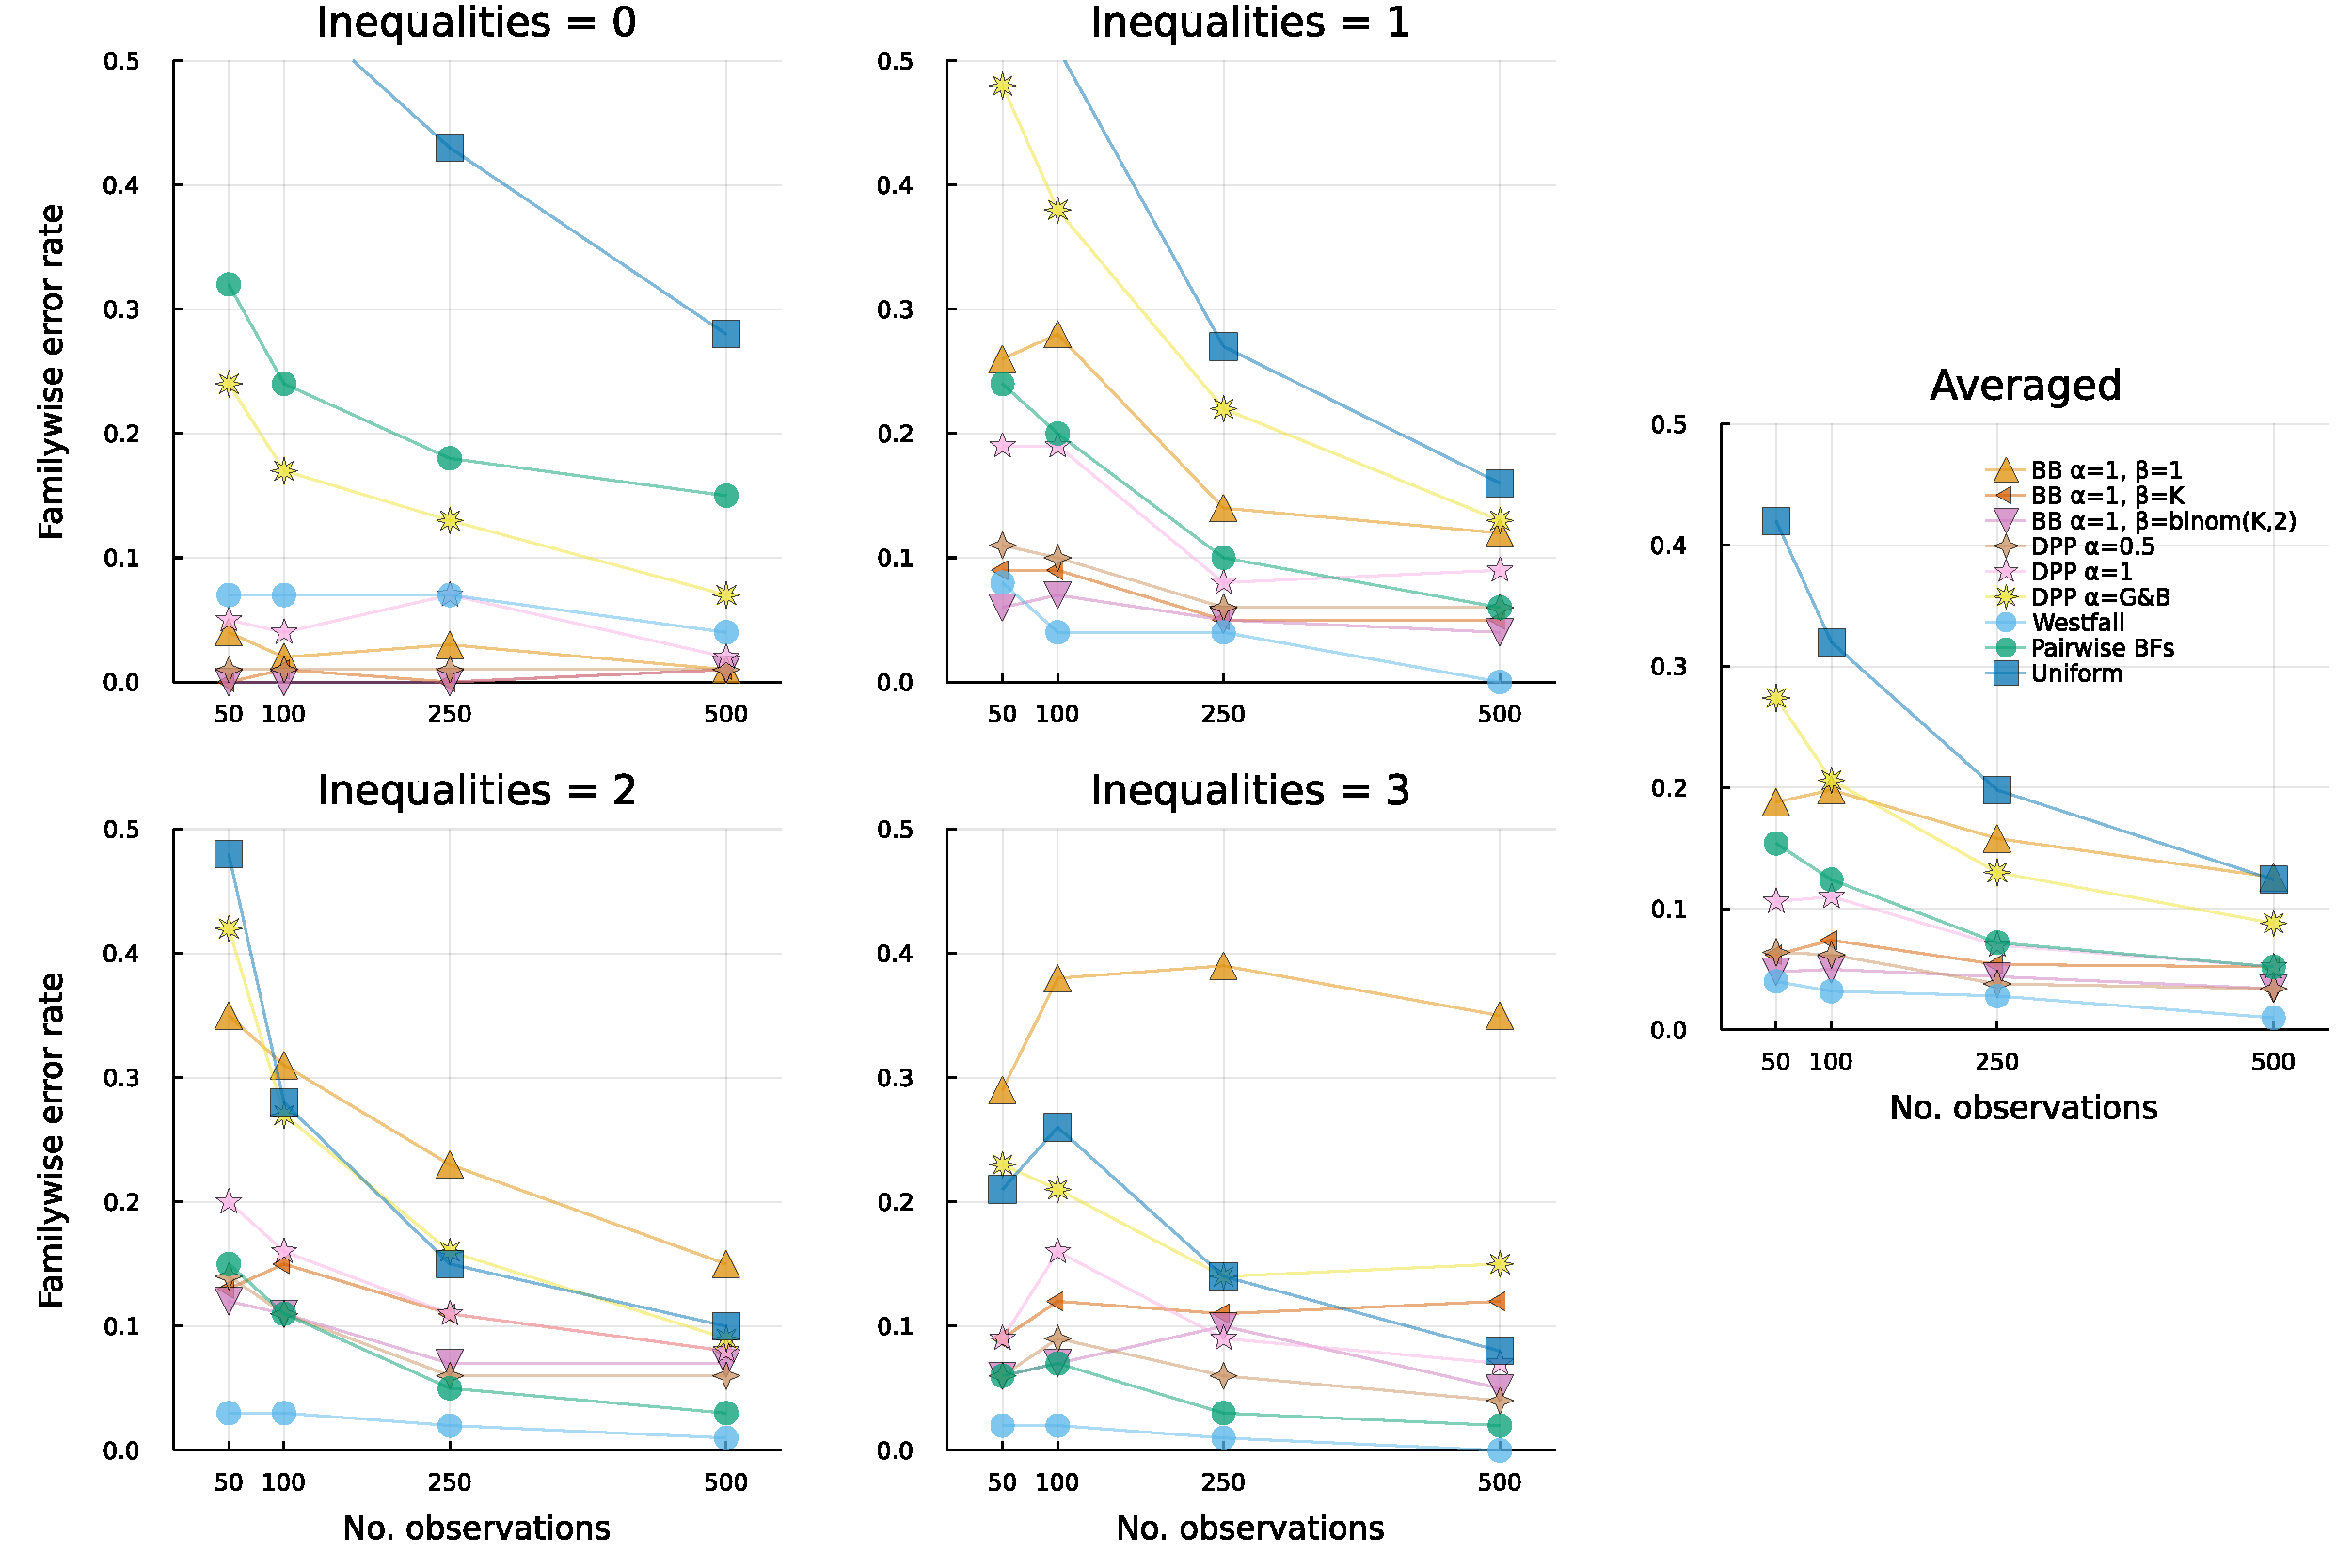
\includegraphics[width=1\textwidth]{subset_k_5_alpha_familywise.pdf}
    \caption{Familywise error rate across priors and sample sizes under a model with 0 (top left), 1 (top right), 2 (bottom left), and 3 (bottom right) true inequalities for $K = 5$ groups. The rightmost panel shows the average familywise error rate across inequalities.}
    \label{fig:big_simulation-I}
\end{figure}

\subsubsection{Statistical Power}
Figure \ref{fig:big_simulation-II} shows the proportion of falsely claiming a difference between two groups when there is none for different methods across the number of \textit{equalities} in the true model and sample sizes. The top left panel shows that the beta-binomial prior with $\beta = 1$ performs best and the method proposed by \textcite{westfall1997bayesian} performs worst, again mirroring the results of the small simulation study above. Increasing the number of equalities in the true model, we find that the performance of virtually all methods decreases except for the uniform prior, which shows a slight increase, especially for large sample sizes. This overall decrease in performance is likely due to the fact that the average pairwise difference between groups \textit{decreases} with the number of equalities. To illustrate, note that the model with no equalities for $K = 4$ groups has population means $\vec{\mu} = \{-0.30, -0.10, 0.10, 0.30\}$, which yields pairwise differences $[0.20, 0.20, 0.20, 0.40, 0.40, 0.60]$ with an average of $0.33$. In contrast, including one equality results in $\vec{\mu} = \{-0.25, -0.05, 0.15, 0.15\}$\footnote{This is due to the sum-to-zero constraint and the constraint that all successive unequal groups have a difference of $0.20$.}, yielding pairwise differences of $[0.20, 0.20, 0.20, 0.40, 0.40]$ with an average of $0.28$.

The rightmost panel in Figure \ref{fig:big_simulation-II} shows the results averaged over the number of equalities in the true model. We find that the method by \textcite{westfall1997bayesian} is highly conservative, trading off the strong familywise error control with an increase in the proportion of false negatives. Similarly, the priors that performed worst with respect to familywise error control — the uniform, symmetric DP, and beta-binomial prior with $\beta = 1$ — perform best here. The other DP and beta-binomial priors as well as the pairwise Bayes factors are somewhere in between those two extremes. Note that again the differences between the methods become less pronounced with increasing sample size.

%the strongest familywise error control, closely followed by the the beta-binomial priors with $\beta = K$ and $\beta = {K \choose 2}$ and the DP prior with $\alpha = 0.50$. The pairwise Bayes factors perform similar to the Dirichlet process prior with $\alpha = 1$, with the beta-binomial prior with $\beta = 1$, the symmetric DP prior, and the uniform prior performing worst.

\begin{figure}[!h]
    \centering
    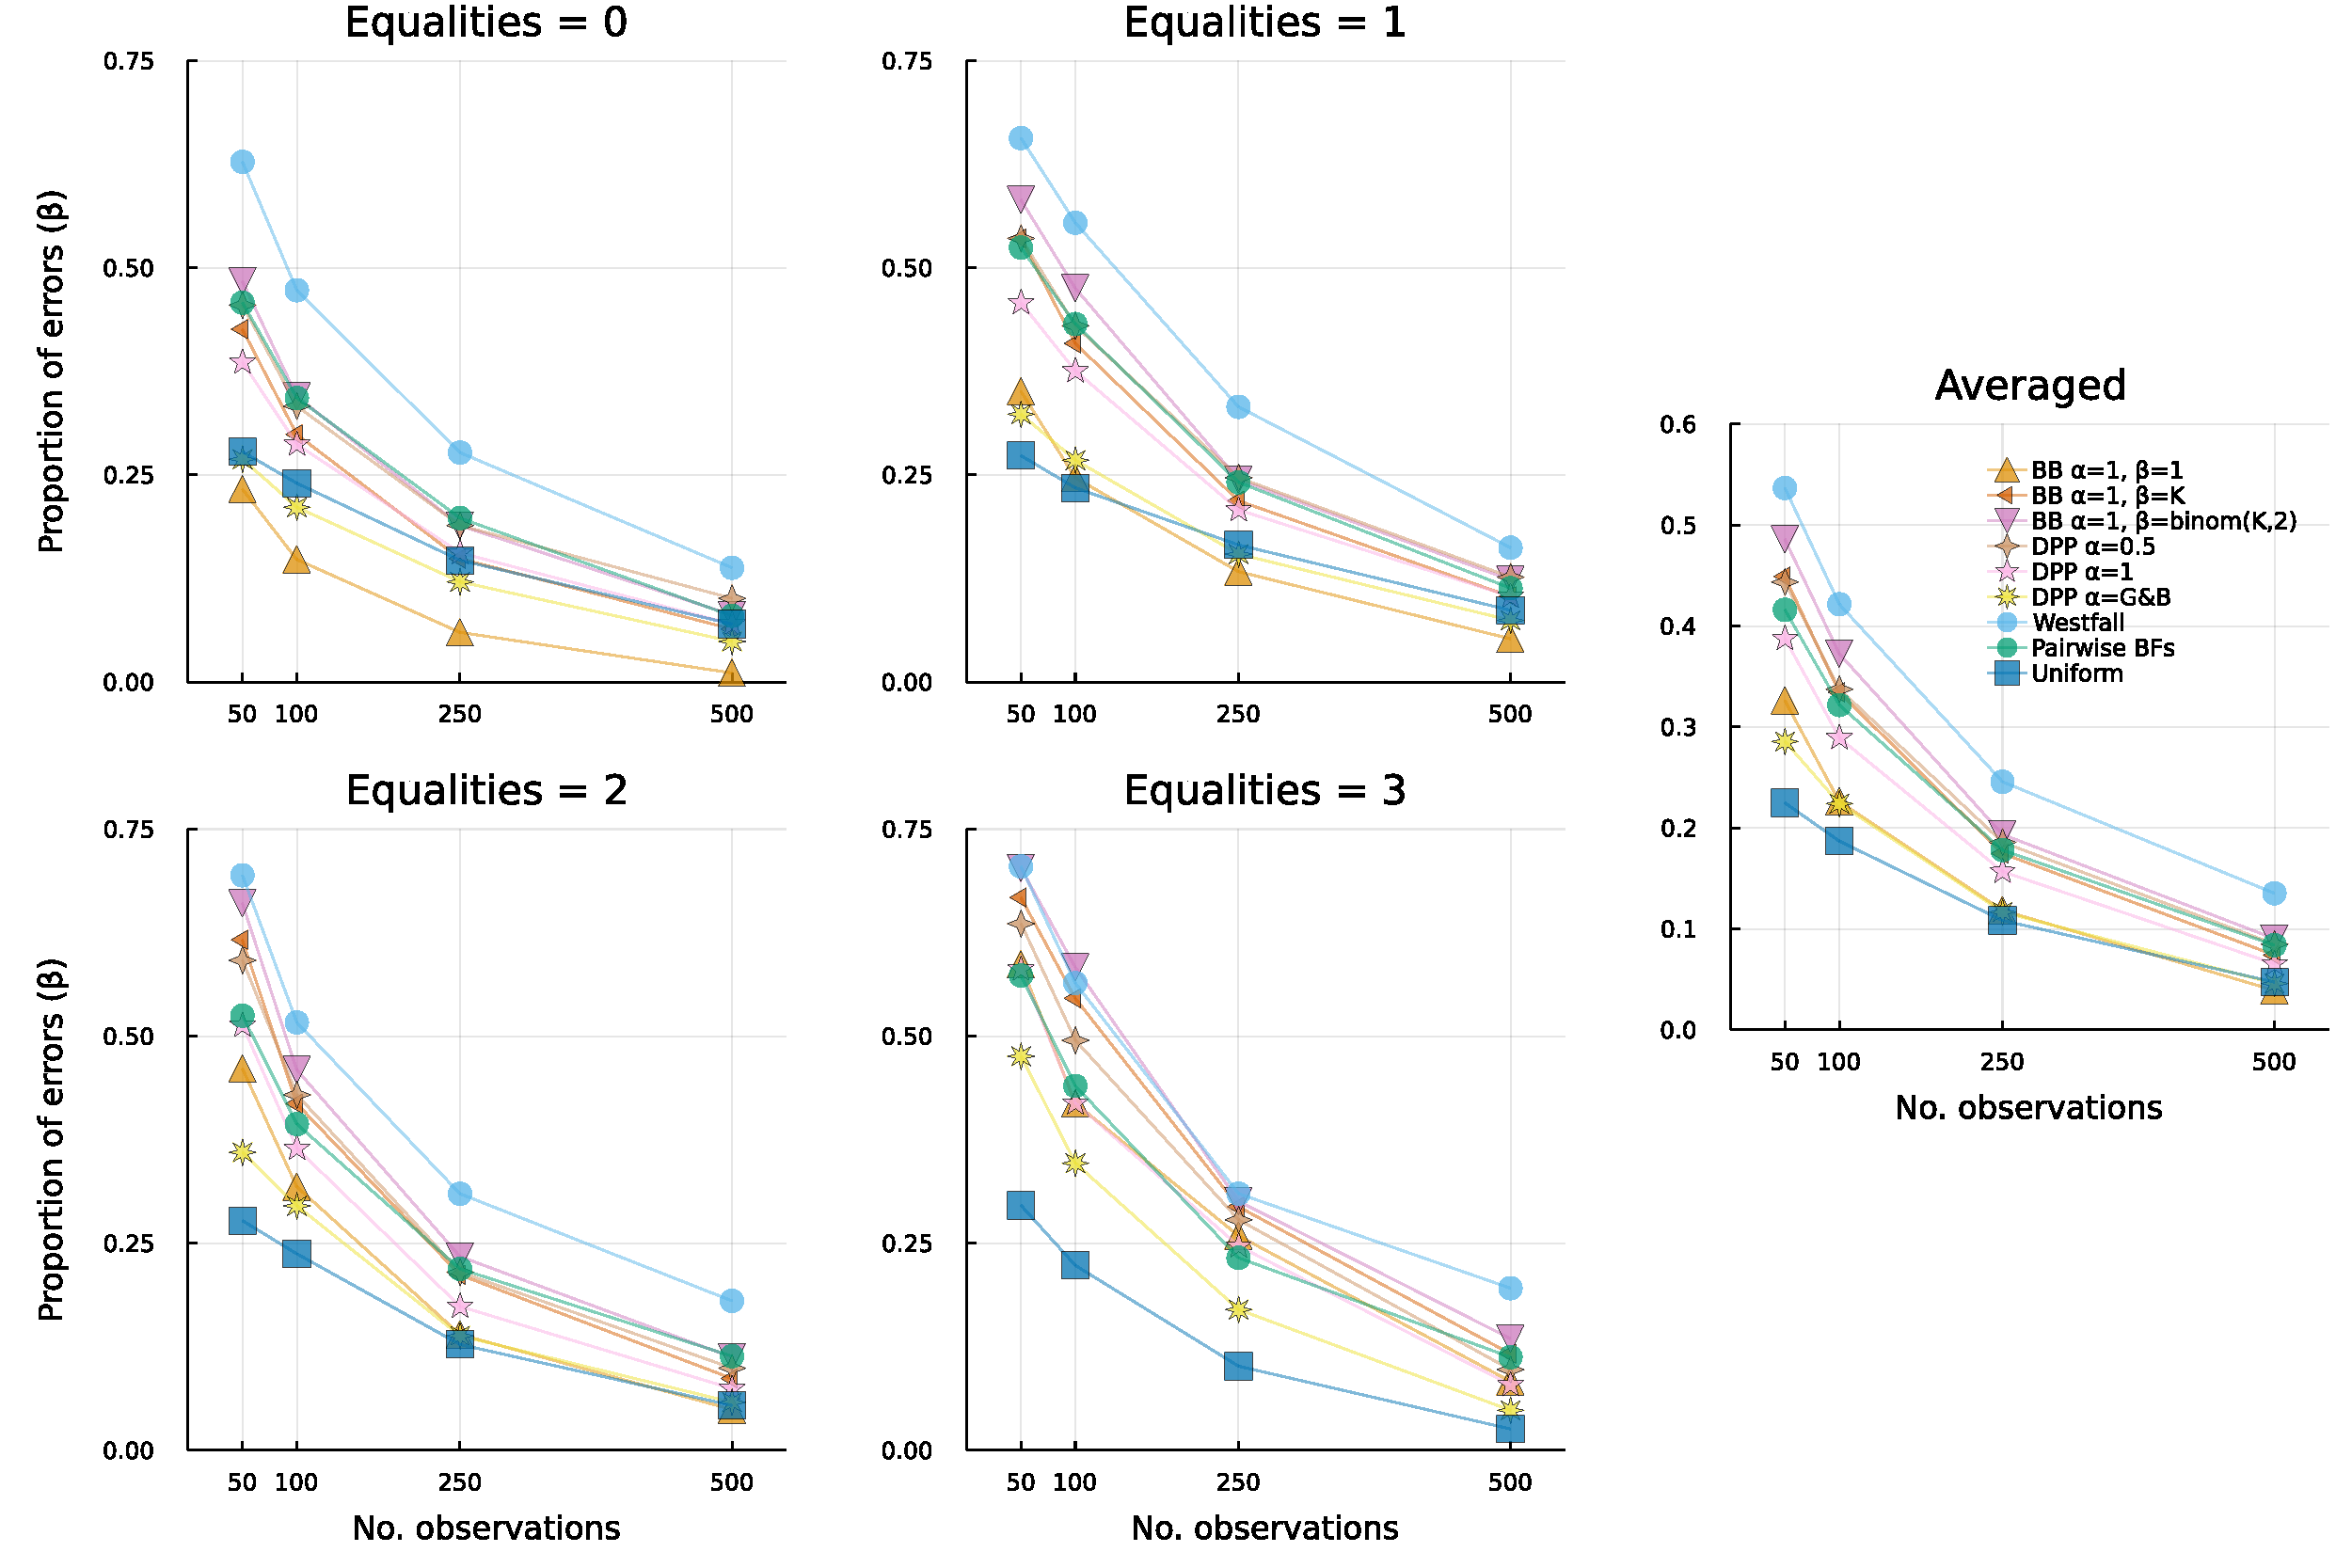
\includegraphics[width=1\textwidth]{subset_k_5_beta.pdf}
    \caption{Proportion of falsely claiming a difference between two groups when there is none across priors and sample sizes under a model with 0 (top left), 1 (top right), 2 (bottom left), and 3 (bottom right) true inequalities for $K = 5$ groups. The rightmost panel shows the average error rate across inequalities.}
    \label{fig:big_simulation-II}
\end{figure}

\subsubsection{Simulation Discussion}
Our results show that no single method dominates all others. While the beta-binomial prior with $\beta = 1$ performed best in our initial simulation study described in Section \ref{sec:illustration}, including models beyond the null and full model showed that this prior performed considerably worse in those settings. The beta-binomial prior with $\beta = K$, $\beta = {K \choose 2}$, and the DP prior with $\alpha = 0.50$ perform very similarly overall. Importantly, both the method proposed by \textcite{westfall1997bayesian} and the pairwise Bayes factors can yield transitivity violations, while explicitly specifying a prior over partitions cannot. For example, we might find that $\mu_1 = \mu_2$ and $\mu_2 = \mu_3$ using pairwise Bayes factors with some threshold, but at the same time conclude that $\mu_1 \neq \mu_3$. This is one key reason why explicitly specifying the prior over partitions is preferable. In the next section, we focus on the beta-binomial prior with $\beta = K$ and apply our method to two examples.

\section{Applications} \label{sec:applications}
In this section, we apply the beta-binomial setup to two examples: testing the (in)equality of proportions and variances, respectively. We have developed a generic Julia package called \textit{EqualitySelection} that utilizes the probabilistic programming framework \textit{Turing} to allow the user to adjust for multiplicity as proposed in this paper. %The code to reproduce the results is given in Appendix \ref{sec:appendix-code}.


\iffalse
\subsection{Testing Means}
Intrusive memories after a traumatic experience can noticeably affect somebody's mental health. \textcite{james2015computer} tested whether intrusive memories can be reduced by a simple cognitive task after memory consolidation. In particular, they had people watch a scary movie and after seven days report the number of intrusive memories they had. There were four experimental conditions applied one day after the scary movie, to allow for the memory to be consolidated. In the ``no-task'' control group, participants completed a filler task after watching the scary movie; in the ``Tetris only'' group, participants played Tetris; in the ``Reactivation only'' group, participants were presented with images from the scary movie; and, lastly, the ``Reactivation + Tetris'' condition had participants play Tetris after the reactivation task.

% http://environmentalcomputing.net/analysis-variance-single-factor/
% https://crumplab.github.io/statistics/anova.html

%\textcite{gopalan1998bayesian} analyze a nice $k = 6$ ANOVA data set but with only $n = 5$ per group.

\FD{Problem is that it's count data ... hmmm.}
\FD{Since we already have a Demo using the ANOVA model, we could leave this out.}
\fi

%\textcite{tong2008too} have five groups rate attractiveness of Facebook users with 100, 300, 500, 700, 900 friends, respectively. Nice example, but a bit dated; it's in JASP.

\subsection{Testing Proportions}
\textcite{nuijten2016prevalence} investigated a sample of 30,717 articles published between 1985 and 2013 in eight major psychology journals for statistical reporting errors. Our question here is: Which journals make the same amount of errors, and which make more errors? We answer the question using the following model specification. For journal $j$, denote the number of statistical errors found as $e_j$ and the number of statistical tests analyzed as $n_j$. We assume that underlying each proportion there is a latent true chance of making an error, $\theta_j$. Thus, we modeled the data as independent binomials, that is, $e_j \sim \mathrm{Binomial}\left(\theta_j, n_j\right)$. Next, we specify a hierarchical level over the partitions to assess for which journals the chances of making an error are equal. This leads to the following model specification:
\begin{align*}
    e_j                 &\sim \mathrm{Binomial}\left(\theta_j, n_j\right)\\
    \theta^u_j          &\sim \text{Beta}(1, 1)\\
    \theta_j            &\leftarrow \text{mean of elements of } \theta^u_j \text{ in the same partition }\\
    % \theta_j            &\leftarrow \theta^u_i \quad\text{ iff } j \in \rho_i\\
    \rho                &\sim \text{beta-binomial}(1, 8) \enspace . \numberthis
\end{align*}
The unconstrained chances $\theta^u_j$ are assigned beta priors from which — together with the partitions — the possibly constrained chances are created. Two chances $\theta_i$ and $\theta_j$ are equal if and only if their indices appear in the same partition $\{i, j\} \subseteq \rho_k$ for some $k$. Note that the model reduces to the full model of independent binomials whenever the partitions state that all elements in $\vec{\theta}$ are distinct. We use a beta-binomial prior with $\alpha = 1$ and $\beta = 8$. The top left panel in Figure~\ref{fig:demo_proportions} shows the posterior distributions for the underlying error chance for each journal under a model that assumes that they are all different.

\begin{figure}
    \centering
    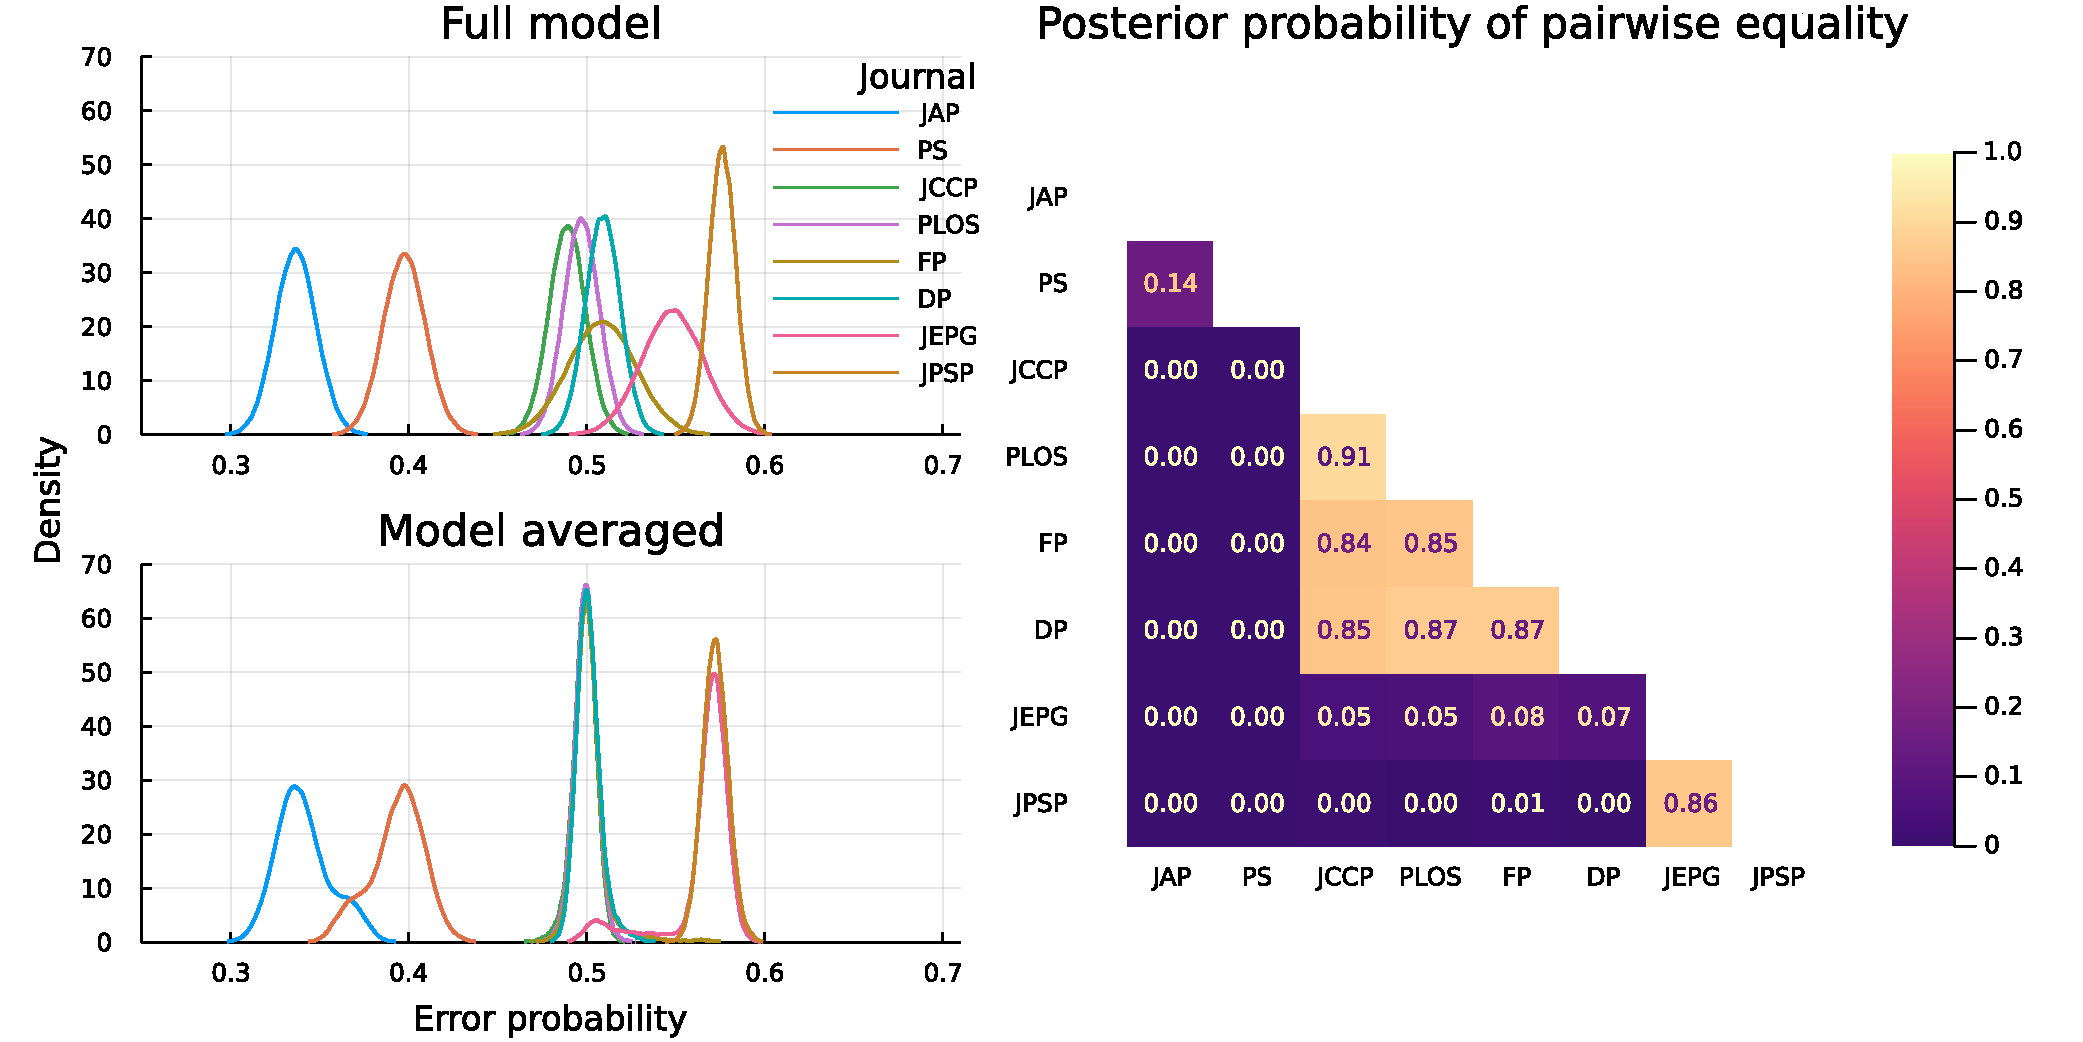
\includegraphics[width=\textwidth]{application_proportions_2panel_plot.pdf}
    \caption{Left: Posterior means of the full model where all proportions are assumed to be different (top) and posterior means when averaging over all models using a beta-binomial($\alpha = 1$, $\beta = 8$) prior (bottom). Right: Posterior probabilities for pairwise equality across all journals. The abbreviations stand for:
    \emph{Journal of Applied Psychology} (JAP), \emph{Psychological Science} (PS), \emph{Journal of Consulting and Clinical Psychology} (JCCP), \emph{ Public Library of Science} (PLOS), \emph{Developmental Psychology} (DP), \emph{Journal of Experimental Psychology: General} (JEPG), and \emph{Journal of Personality and Social Psychology} (JPSP).}
    \label{fig:demo_proportions}
\end{figure}

We can see that the posterior distributions for JCCP (green), PLOS (purple), DP (turquoise), and FP (beige) are very close to each other, with FP showing more pronounced uncertainty. The panel below shows the model-averaged posterior distributions, clearly demonstrating a shrinkage effect. The error chances for JAP and PS are pulled toward each other, with JCCP, PLOS, DP, and FP being shrunk towards each other almost completely, similarly to JEPG and JPSP. The right panel in Figure~\ref{fig:demo_proportions} gives the posterior distributions for pairwise equality across all journals, reflecting the two main clusters in the model-averaged density plot on the left.

%\FD{The shrinkage seems really strong actually. How does it look for the DP? Fabian runs it! I ran it and the shrinkage is quite extreme also with the DP (for all values of $\alpha$, see demo-proportions-joined-density-plots.pdf; even the uniform prior shows some shrinkage ...}

%of allowing different error chances to be equal. The left panel shows the results for the full model --- the observer proportions and posterior means are in near perfect agreement. The right panel shows the results for a default beta-binomial prior with $\alpha = 8$, $\beta = 1$ prior, illustrating that adjusting for multiplicity introduces shrinkage in the parameter estimates towards each other.

%\FD{How is the model implemented? Is it like ANOVA, but on proportions? Then it would be log linear analysis. \textcite{gopalan1998bayesian} just compare proportions, for example. It seems that the Bayesian loglinear analysis in JASP (due to Overstall \& Forster) does model averaging, so in a sense it should be very similar to our approach. It also makes more sense conceptually, see the example below.}
%\textcite{radelet1991choosing} study decisions on death penalties (yes / no) by race of defendant (black / white) and race of victim (black / white). This yields 6 cells, data are in JASP. An interaction in a loglinear model would have a particular effect on the posterior equivalence of groups, so there is some relation here. Let's discuss this.

%There is another nice data set about bias in MOOCs due to \textcite{baker2018bias}, but the JASP data set completely ignores variance due to different MOOCs, instructors, etc. So it's a completely inadequate analysis.


\subsection{Testing Standard Deviations}
\textcite{borkenau2013sex} studied whether men and women differ in the variability of personality traits. Here we focus on five personality traits (agreeableness, extraversion, openness, conscientiousness, neuroticism) rated by participants' peers in an Estonian sample consisting of $n_1 = 969$ women and $n_2 = 716$ men. Our goal is to assess which personality traits across the sexes can be assumed equal in terms of their variability. This example shows how our methodology can be used to test group differences while taking the multivariate dependency of the outcome measure into account. We build on the parameterization proposed by \textcite{dablander2020default}, who developed a default Bayes factor test for testing the (in)equality of variances. Let $\vec{y}_1$ and $\vec{y}_2$ denote the five-element vectors of observed data for men and women, respectively, and $K = 10$ be the total number of variables. For each sex $k \in \{1, 2\}$, we have:
\begin{align*}
    \vec{Y}_k         &\sim \mathcal{N}\left(\vec{\mu}_k, \Sigma_k \right)\\
    \vec{\mu}_k       &\propto \vec{1}  \\
    \Sigma_k          &= \text{diag}(\vec{\sigma}_k) \, \Omega_k \, \text{diag}(\vec{\sigma}_k) \\
    \Omega_k          &\sim \text{LKJ}(1) \enspace ,
\end{align*}
where LKJ refers to the Lewandowski-Kurowicka-Joe prior \parencite{lewandowski2009generating}. To test the equality of variances both between and across groups, we define the ten-variable standard deviation vector $\vec{\sigma} = [\vec{\sigma}_1, \vec{\sigma}_2]$ with $\bar{\sigma}$ denoting the average standard deviation. Following \textcite{dablander2020default}, we write $\sigma_j = \left(K\vartheta_j\bar{\sigma}\right)^{-1}$, where $\vartheta_j = \nicefrac{\sigma_j}{\sum_{j = 1}^K \sigma_j}$ is the relative standard deviation and $\vartheta_K = 1 - \sum_{j = 1}^{K - 1} \vartheta_j$. To complete the model specification, we write:
\begin{align*}
    \sigma_j     &= \left(K\vartheta_j\bar{\sigma_j}\right)^{-1} \\
    % \tau_j        &= \left(K\vartheta_j\bar{\tau}\right)^{-1} \\
    % \bar{\tau} &\propto \bar{\tau}^{-1} \\
    \bar{\sigma}_j &\propto \bar{\sigma}_j^{-1} \\
    % \vartheta_j       &\leftarrow \vartheta^u_i \quad\text{ iff } j \in \rho_i\\
    \vartheta_j            &\leftarrow \text{mean of elements of } \vartheta^u \text{ in the same partition }\\
    \vec{\vartheta}^u     &\sim \text{Dirichlet}(1, \ldots, 1) \\
    \rho              &\sim \text{beta-binomial}(1, 10) \enspace . \numberthis
\end{align*}
Two standard deviations $\sigma_i$ and $\sigma_j$ are equal if and only if their indices appear in the same partition $\{i,j\}\subseteq\partition_k$ for some $k$.
When the partition states that all standard deviations are distinct we recover the full model. % I added this because we also said this for the binomial example
The top left panel of Figure~\ref{fig:demo_variances} shows the posterior distributions under the full model that assumes all standard deviations are different.
\begin{figure}
    \centering
    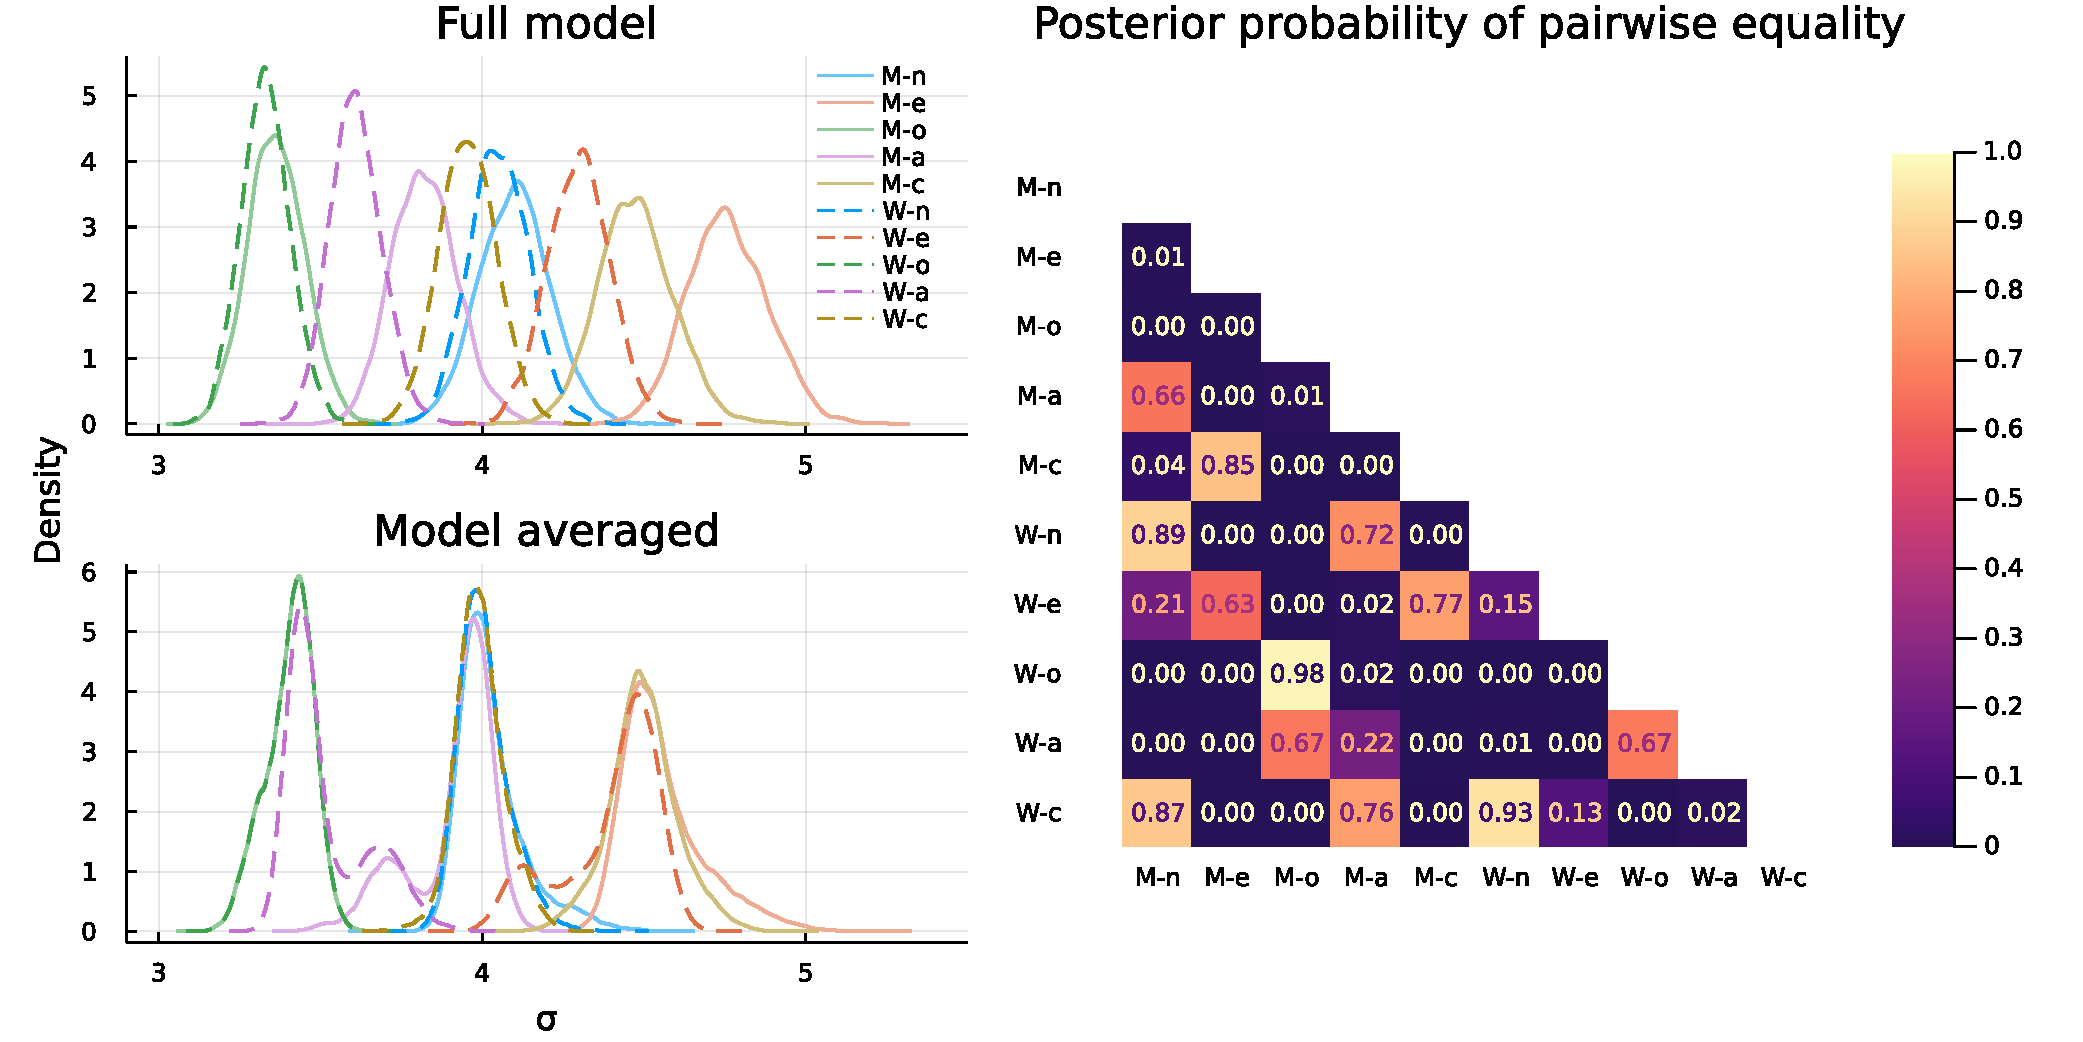
\includegraphics[width=\textwidth]{demo_variances_2panel_plot.pdf}
    \caption{Left: Posterior means of the full model where all standard deviations are assumed to be different (top) and posterior means when averaging across all models using a beta-binomial($\alpha$ = 1, $\beta$ = 10) prior (bottom).
    Right: Posterior probabilities for pairwise equality across all personality traits. In the abbreviations the first letter stands for \emph{men} (m) or \emph{women} (w). The second letter stands for \emph{neuroticism} (n), \emph{extraversion} (e), \emph{openness} (o), \emph{agreeableness} (a), and \emph{conscientiousness} (c).}
    \label{fig:demo_variances}
\end{figure}

While all posterior distributions lie close to each other, the standard deviations of openness for men and women overlap particularly much. The bottom panel shows the model-averaged posterior distributions, which again demonstrate a shrinkage effect. The right panel of Figure~\ref{fig:demo_variances} shows the posterior probability of pairwise equality across all personality traits for men and women. It appears that there are three clusters: (1) men--openness, women--openness, and women--agreeableness; (2) men--neuroticism, women--neuroticism, women--conscientiousness, and men--agreeableness; (3) men--conscientiousness, men--extraversion, and women--extraversion. However, for the personality traits women--agreeableness, men--agreeableness, and women--extraversion, the evidence is not overwhelming, as indicated by the bimodality in the model-averaged posterior distributions.

%\textcite{boos2004comparing} reanalyze a data set with 8 groups concerning pheromones and flowers reported in \textcite{groot2005effect}; pretty boring, but something like this we need. Hmm, but they only report absolute deviation from the mean, not the sample variances. See \url{https://www.tandfonline.com/doi/abs/10.1080/03610918.2018.1485937?journalCode=lssp20} for variance test from 1994 on four groups.
% https://onlinelibrary.wiley.com/doi/full/10.1002/ldr.2816

\section{Discussion} \label{sec:discussion}

% Summary paragraph
Testing the (in)equality between groups while adjusting for multiple comparisons is a core challenge in many applied settings. In this paper, we have proposed a flexible class of beta-binomial priors to penalize multiplicity and make inferences over all possible (in)equalities in relatively general settings. We compared the beta-binomial priors to a Dirichlet process prior suggested by \textcite{gopalan1998bayesian}, to a uniform prior, to the method proposed by \textcite{westfall1997bayesian}, and to an uncorrected method based on pairwise Bayes factors. We also illustrated our method, which is freely available in the Julia package \textit{EqualitySelection}, on two examples.

% Implications
We found that a beta-binomial prior with $\alpha = 1$ and $\beta \in \{K, {K \choose 2}\}$ as well as a Dirichlet process prior with $\alpha < 1$ adequately control the familywise error rate, while a uniform prior and using only pairwise Bayes factors, unsurprisingly, do not. We also found that the method proposed by \textcite{westfall1997bayesian} compares favorably in terms of error control but not in terms of power. While we have focused on a posterior probability threshold of $0.50$ (i.e., a Bayes factor of 1), other thresholds will naturally impact the trade-off between the two types of errors. Importantly, and in contrast to conventional adjustments for multiple comparisons \parencite[e.g.,][]{westfall1997bayesian, jeffreys1961theory}, specifying a prior over the partitions allows inferences over all possible (in)equalities. This means that researchers can use the methods we provide to assess not only the probability of pairwise (in)equalities --- as is common in standard post-hoc tests for, say, ANOVA --- but in fact can make probabilistic statements over any set of (in)equalities they wish to assess. Similarly, the outlined approach also allows for model-averaging, which as we have seen in the applications yields shrinkage of the groups towards each other. Using a prior over partitions further avoids violations of transitivity, i.e. claiming for example that $\mu_1 \neq \mu_3$ while both $\mu_1 = \mu_2$ and $\mu_2 = \mu_3$.

%Simulation study two looks at the problem: first only from null model across increasing group sizes, second fixing group size across sample size and equalities ...
%Reflection on transitivity violation of pairwise methods
%Reflection on shrinkage versus testing (?), Gelman

% Limitations
As with any statistical method, there are a number of points to keep in mind. First, while we suggest default values of $\alpha = 1$ and $\beta = K$ for the beta-binomial prior and $\alpha \leq 1$ for the DP prior, researchers may wish to use a more informed prior specification. Values for the prior parameters can be elicited by specifying model priors for two out of the following: the prior on the null model, on the full model, or their ratio. Second, the beta-binomial prior differs from the DP prior in that it assigns models with the same number of partitions the same prior probability, while the DP prior assigns more mass to the model with the larger cluster. It is not obvious which of the two behaviors is more desirable, and it may well depend on the problem under study. Researchers using the methods we have made available should keep this difference in mind, although the extent to which it matters in practice remains to be seen.

%Third, only controlling the probability of incorrectly claiming that two groups are different when in fact they are not is not necessarily the best strategy. Instead, it is important to also study the extent to which the method does not pick up differences that are in fact there. Future research may wish to compare the Dirichlet process and the beta-binomial priors using such a metric. \FD{We should do this simulation study, let's discuss.}

There are some practical limitations of our implementation that we leave for future work. We currently do not allow for factorial designs, for example, for which dummy or contrast coding is more natural. The key challenge there is to specify the prior in such a way that it reflects the structure of the experimental design. For the present, we believe that the Bayesian approach outlined in this paper can help applied researchers who wish to compare multiple groups.

%\paragraph{Acknowledgements.}% Send it to EJ, Maarten, Jeff Rouder, Frederick, Frantisek, Samuel from Switzerland.}

\paragraph{Author Contributions.} DvdB and FD proposed the study. DvdB implemented the method and created the Julia package. DvdB conducted the simulation study and analyzed the data with the help of FD. FD and DvdB wrote the manuscript. All authors read and approved the submitted version of the paper. They also declare that there were no conflicts of interest.


%\textcite{kim2009spiked} combine a spike at zero with a DPP. \textcite{curtis2011bayesian} also use a DPP to combine clustering of highly correlated predictors in linear regression with variable selection. \textcite{canale2017pitman} focus on the Pitman-Yor process, which is a generalization of the DPP. \textcite{lu2018reducing} study a powered Chinese restaurant process. \textcite{miller2015microclustering} study a microclustering property, for which the number of data points in a cluster does not grow linearly with the total number of data points (which is assumed by the DP, PY, etc.)

% We focused on independent groups, but one could model dependencies using the distance CRP \parencite{blei2011distance}.

%The Pitman-Yor process generalizes the DP \parencite{pitman1997two}, but it, too, assumes a ``rich-get-richer'' structure which may be undesirable. Both the DP and the PY are instances of so-called \textit{species-sampling models} (SSM), which are a general class of nonparametric models \parencite[e.g.,][]{lee2013defining, ishwaran2003generalized, pitman1996some}. To keep this paper contained, however, we focus on the DP as the only example of a nonparametric model.

\iffalse
Discussion points:
\begin{itemize}
    \item Factorial designs
    \begin{itemize}
        \item Here a dummy coding is more natural, which does not square with our setup. Maybe fine if we combine offsets?
    \end{itemize}
    \item Dependent observations
    \begin{itemize}
        \item Either a relatively simple (?) change to the likelihood, or a time-series problem
    \end{itemize}
    \item DP and BB partition difference
\end{itemize}
\fi

\iffalse
\subsection{Convergence Rate}
\begin{itemize}
    \item \textcolor{red}{For each prior, simulate from true model and plot posterior probability as sample size increases. Ideally, we see that DP is not consistent.}
\end{itemize}

\FD{We should do this plot just to check the consistency result from above, but I'm not sure whether it should actually be in the paper. I mean, it will just show the (slow) Bayes factor convergence.}

\textcite{chen1995optimal} showed that the optimal rate of convergence in the finite mixture problem when the number of components are unknown is $n^{-\frac{1}{4}}$ (with knowledge of the components, the rate can be $\sqrt{n}$). \textcite{ishwaran2001bayesian} show that a Bayesian estimation method is consistent and achieves the $n^{-\frac{1}{4}}$ convergence rate in finite mixtures with the number of components unknown.

\textcite{miller2014inconsistency} argue that nonparametric clustering using a large class of models is inconsistent; see also \textcite{miller2013simple}, for an example. \textcite{miller2018mixture} therefore suggest mixture models with a prior on the number of components with support $\mathbb{N}$ instead of using a nonparametric approach. See also \textcite{green2001modelling} for a comparison of the two approaches.
\fi


\printbibliography

\newpage
\appendix

\iffalse
\section{Prior Comparison} \label{sec:scott-berger}
Figure~\ref{fig:scott_berger} illustrates the penalty imposed by the priors for including an additional inequality constraints into a model. The panels in the top row show the (log) prior probability of a model with a specific number of inequalities for a fixed number of groups $K = 30$ across the different priors. For the Dirichlet process prior, the prior probability is not uniquely determined by the number of inequality constraints (as illustrated in Figure~\ref{fig:prior-comparison}) and we therefore show the average prior probability of a model with a particular number of inequality constraints. As above, we see that the DP with $\alpha < 1$ and the beta-binomial prior with $\beta = K$ show a monotonically decreasing trend as the number of inequality increases, while the uniform prior assigns equal prior mass to the models. \FD{Decide on BB parameterization.}

The panels in the bottom row show the prior odds of including additional inequality constraints as a function of how many inequalities are already present and the number of groups $K$. For example, the blue line shows the prior odds of going from a model with no inequalities ($P(\#0)$) to a model with one inequality ($P(\#1)$). For both the DP (left) and the beta-binomial prior (right), the prior odds in favor of the null model show a similar pattern — they increase linearly with the number of groups. In contrast, the uniform prior (right) gives equal prior odds across all group sizes. Note that the prior odds ratio value on the blue line for $K = 30$ corresponds to the exponentiated difference between the log prior values at 0 and 1 in the top panels. \FD{Create points to make this visually clear in the figure?}

While the blue lines in the bottom panel of Figure~\ref{fig:scott_berger} show the prior odds of going from the null model to a model with one inequality, the orange lines show the prior odds of going from a model with one inequality to one with two inequalities, the green lines from going from one with four to one with five, and the purple lines from going to nine to one with ten. We see that, as the number of already existing inequalities increases, the penalty for including an additional one decreases. This is also encoded in the top panels, which for the DP and the beta-binomial prior show a less steep decrease as the number of inequalities increases.

\begin{figure}
    \centering
    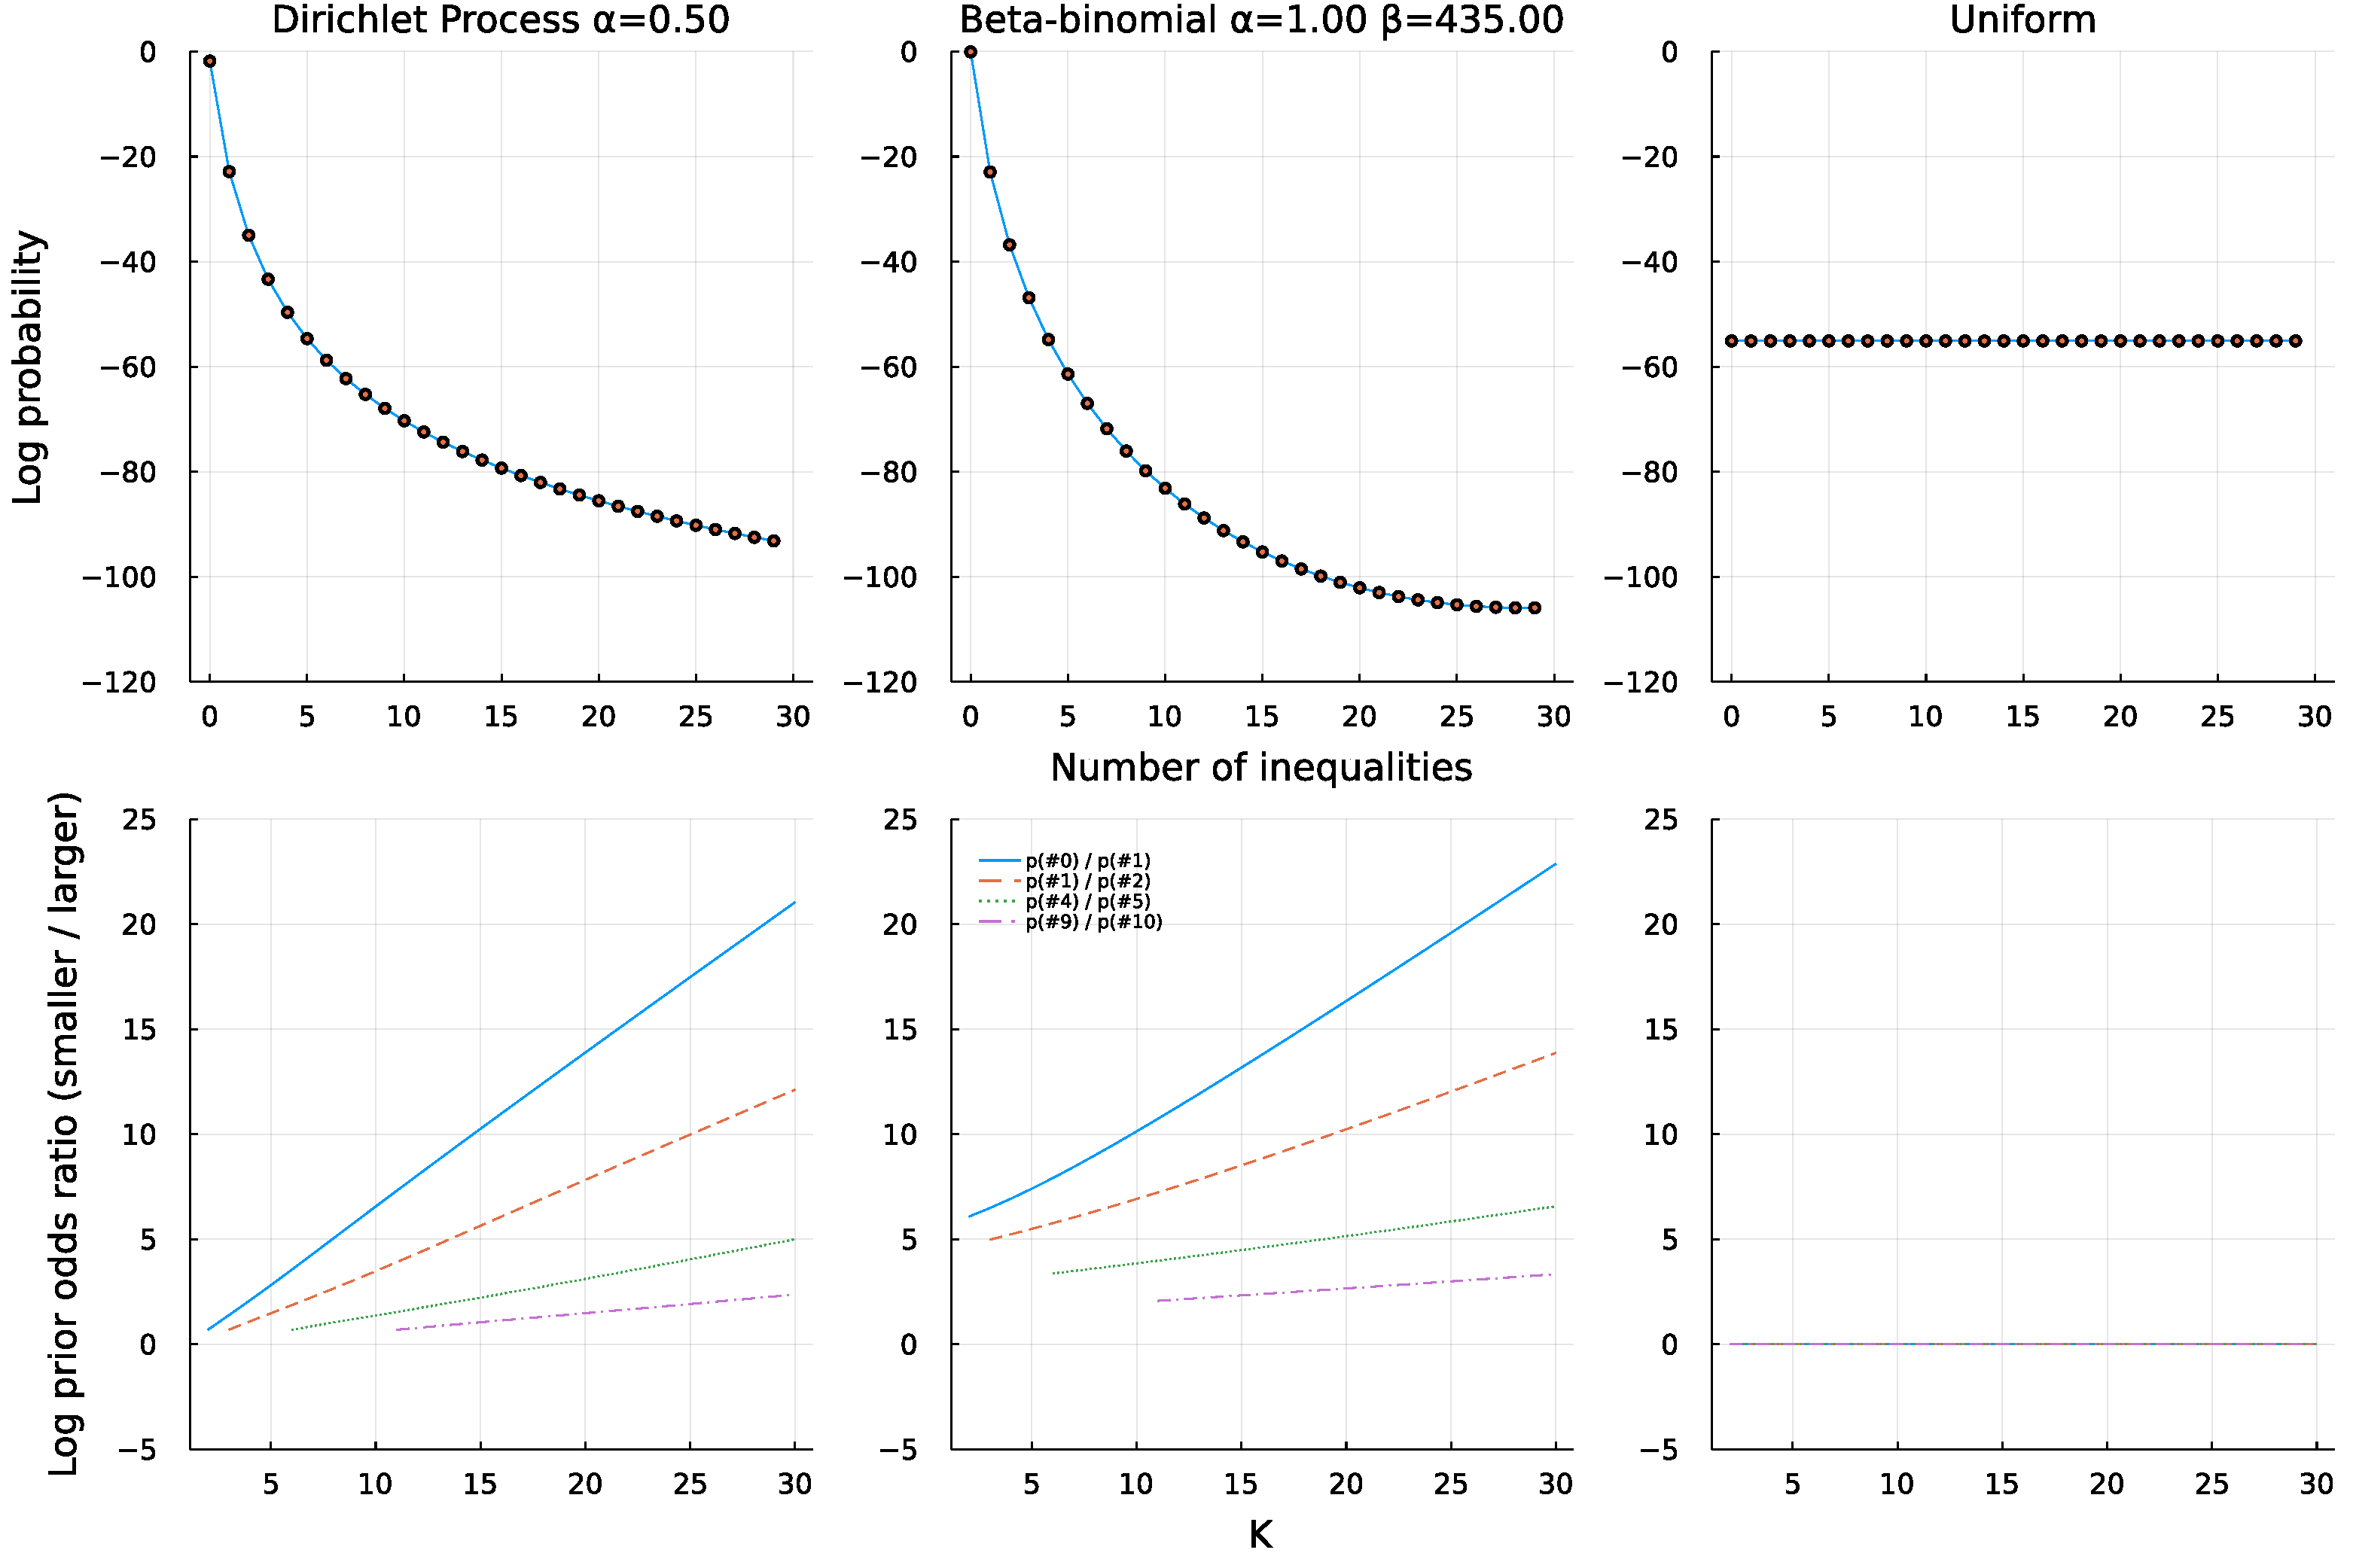
\includegraphics[width=0.89\textwidth]{prior_comparison_plot_2x3_log_scale.pdf}
    \caption{Top: Penalty imposed by the Dirichlet process, uniform, and beta-binomial priors for including additional inequality constraints. Shows log prior probability of the number of inequalities in the model for $K = 30$. Bottom: Shows the prior odds of adding one additional inequality to a model as a function of how many inequalities already exist (0: blue, 1: orange, 4: green, 9: purple) as a function of the number of groups $K$.}
    \label{fig:scott_berger}
\end{figure}
\fi

\iffalse
\section{Example Code} \label{sec:appendix-code}
Using the Julia language, the code below reproduces the results in Section \ref{sec:applications}.

\begin{minted}{Julia}
import Pkg
Pkg.add("EqualitySampler")
using EqualitySampler

# Show the one_way_anova call
# Show the proportion_test call
\end{minted}
\fi

\iffalse
\noindent This can also be done from R, as the code below demonstrates.

\begin{minted}{R}
devtools::install_github('vandenman/EqualitySelection')
library('EqualitySelection')
\end{minted}
\fi

\iffalse
\newpage
\begin{figure}
    \centering
    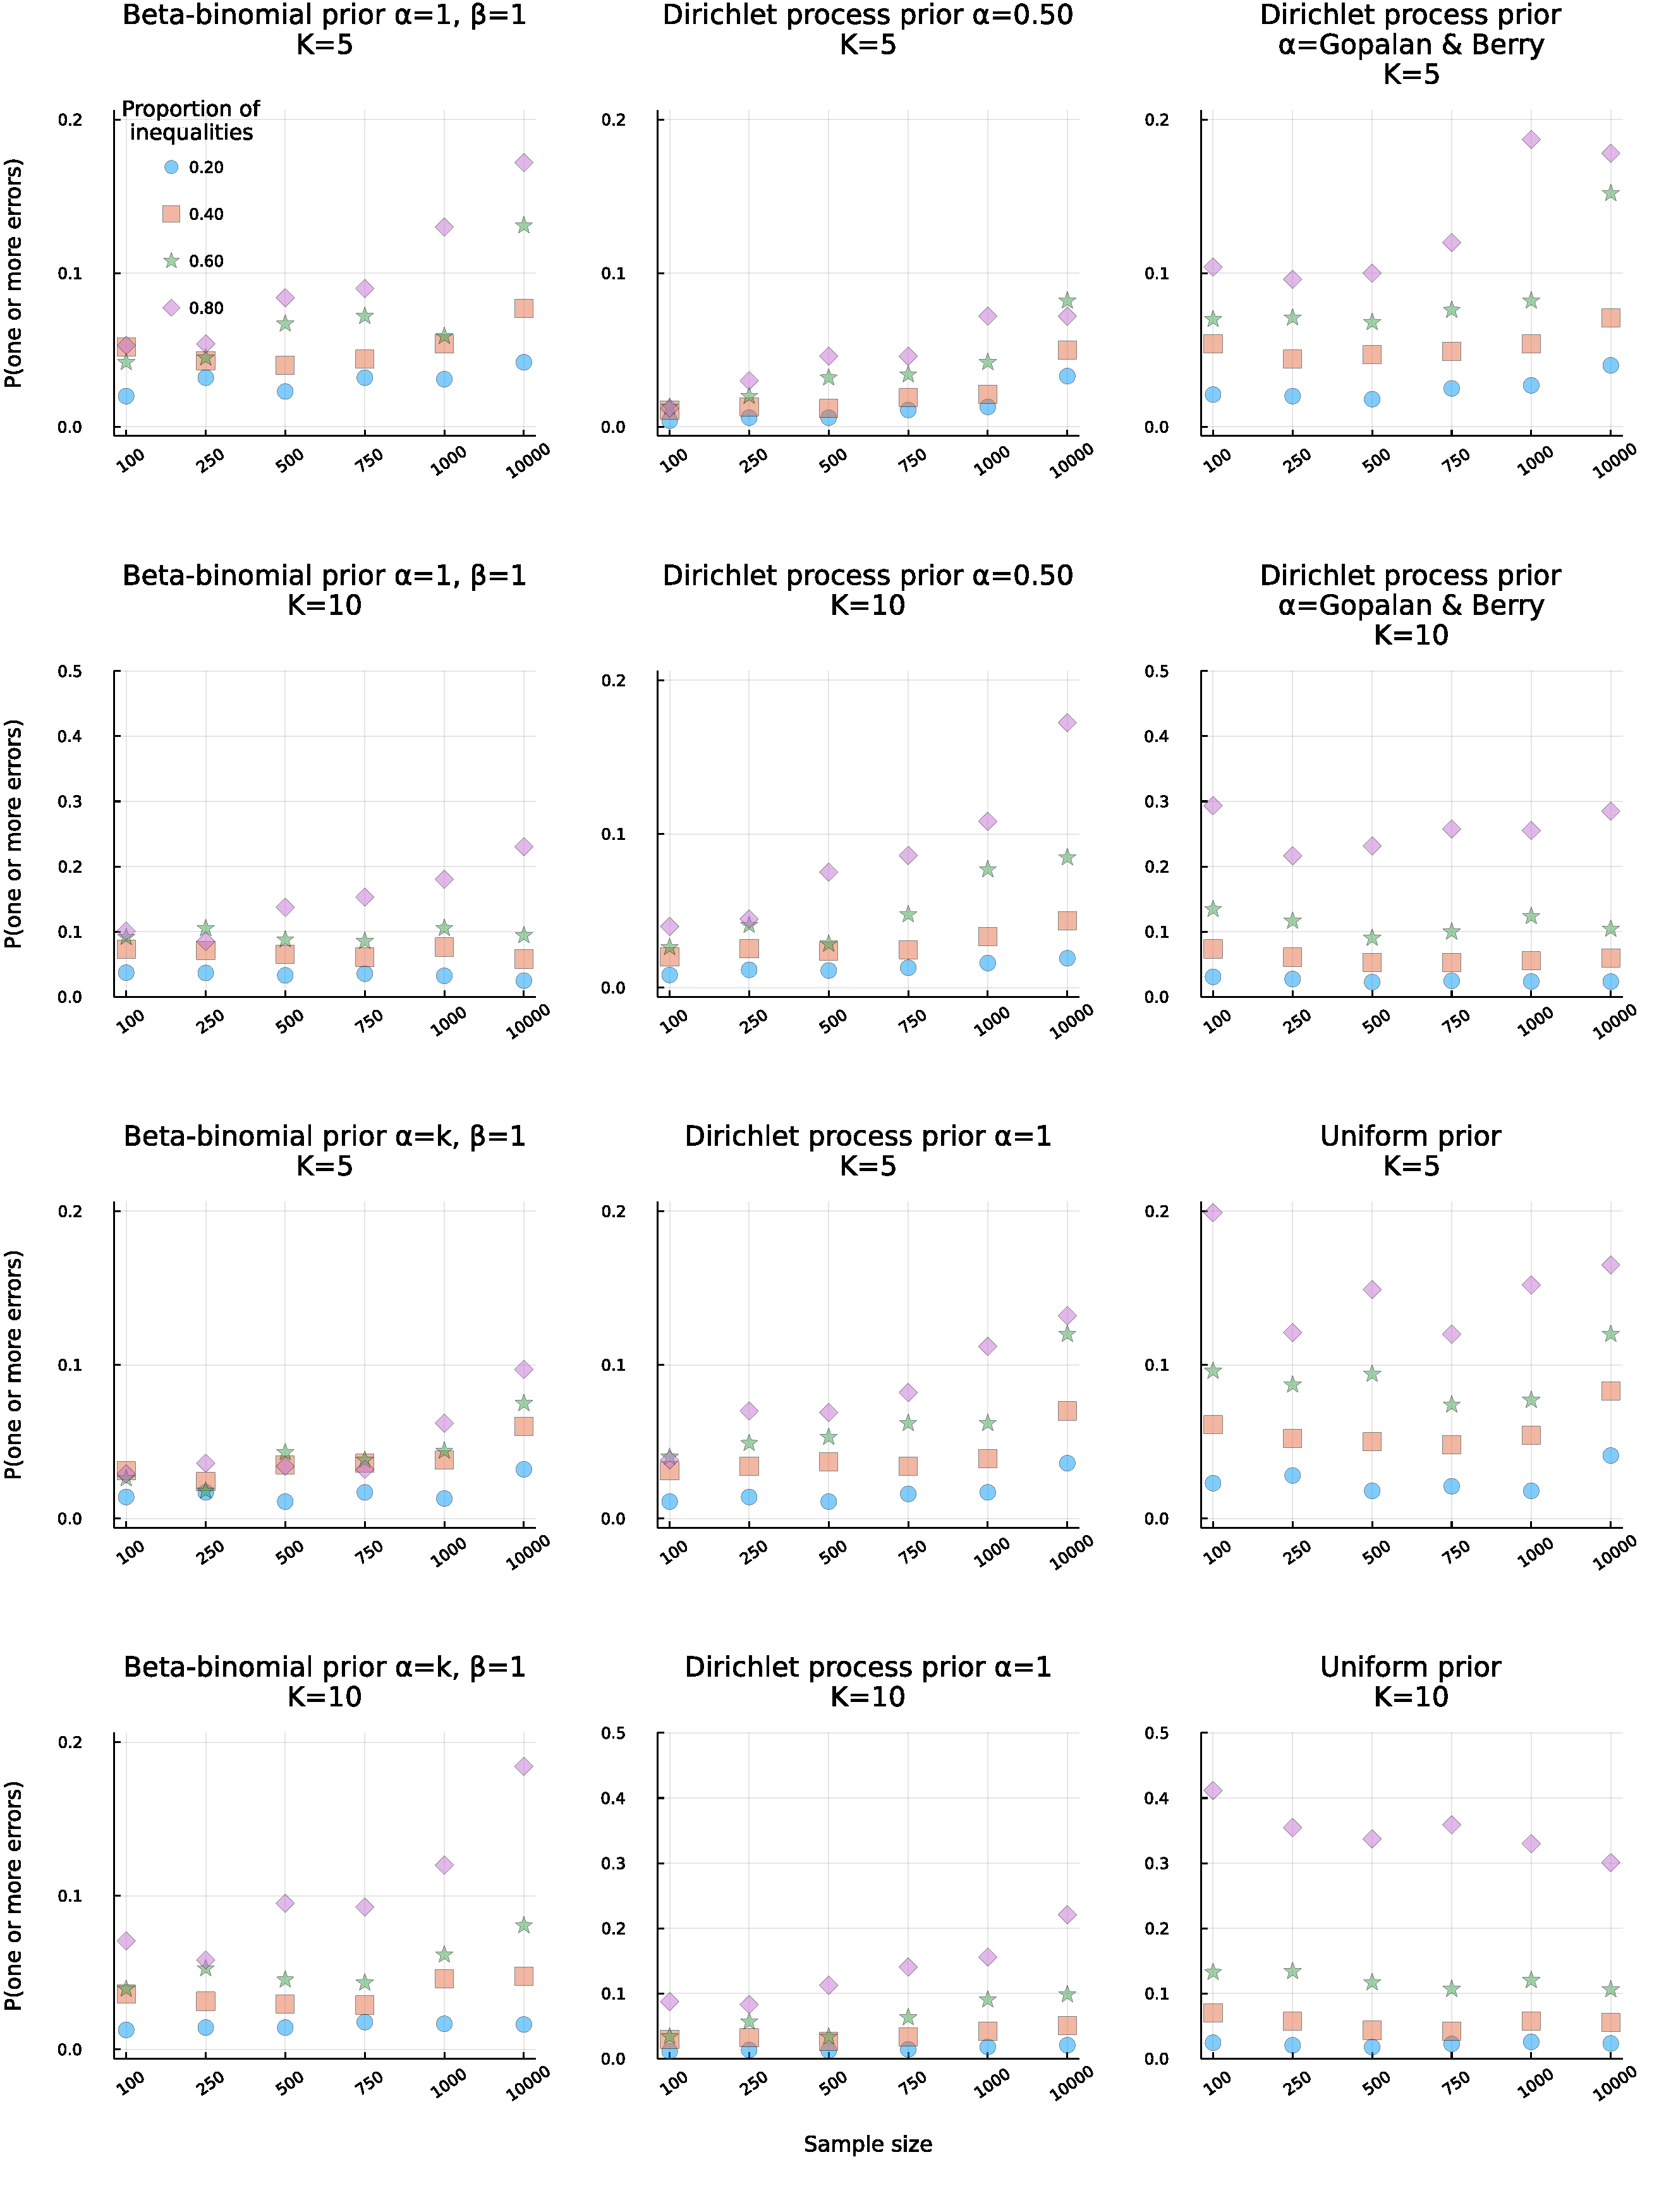
\includegraphics[width=\textwidth]{simulation_results_test_clean_figures/simulation_appendix.pdf}
    \caption{Proportion of false inequalities recovered across all simulations.}
    \label{app_fig:big_simulation}
\end{figure}
\fi

\section{Beta-binomial Prior with Decreasing Prior Model Odds} \label{ap:decreasing-odds}
\begin{prop}\label{prop:monotonicity}
The prior density of the beta-binomial distribution over partitions is decreasing for $\alpha = 1$ and $\beta \geq \binom{K}{2}$, and strictly decreasing for $\alpha = 1$ and $\beta > \binom{K}{2}$.
\end{prop}

\iffalse
\begin{proof}
Recall the beta-binomial prior over partitions:
\begin{equation}
    \pi(\rho \mid K, \alpha, \beta) = \binom{K - 1}{|\rho| - 1}
    \frac{\FBeta{|\rho| - 1 + \alpha}{K - |\rho| + \beta}}
    {\FBeta{\alpha}{\beta}\stirling{K}{|\rho|}} \enspace .
\end{equation}
Fixing $\alpha = 1$, our goal is to find values for $\beta$ such that a partition of size $|\rho| + 1$ (under the condition that $|\rho| + 1 \leq K$) is assigned at least as much prior probability than a partition of size $|\rho|$. We write:
\begin{align}
    \binom{K - 1}{|\rho|}
    \frac{\FBeta{|\rho| + 1}{K - |\rho| - 1 + \beta}}
    {\FBeta{1}{\beta}\stirling{K}{|\rho| + 1}} &\geq \binom{K - 1}{|\rho| - 1}
    \frac{\FBeta{|\rho|}{K - |\rho| + \beta}}
    {\FBeta{1}{\beta}\stirling{K}{|\rho|}} \\[0.50em]
    \frac{\FBeta{|\rho| + 1}{K - |\rho| - 1 + \beta}\stirling{K}{|\rho|}}
    {\FBeta{|\rho|}{K - |\rho| + \beta}\stirling{K}{|\rho| + 1}} &\geq \frac{|\rho|}{K - |\rho|} \\[0.50em]
    \frac{\FGamma{|\rho| + 1}\FGamma{K - |\rho| - 1 + \beta}\stirling{K}{|\rho|}}
    {\FGamma{|\rho|}\FGamma{K - |\rho| + \beta}\stirling{K}{|\rho| + 1}} &\geq \frac{|\rho|}{K - |\rho|} \\[0.50em]
    \frac{|\rho|\stirling{K}{|\rho|}}
    {(K - |\rho| + \beta - 1)\stirling{K}{|\rho| + 1}} &\geq \frac{|\rho|}{K - |\rho|} \\[0.50em]
    \frac{\stirling{K}{|\rho|}}
    {\stirling{K}{|\rho| + 1}} &\geq \frac{K - |\rho| + \beta - 1}{K - |\rho|} \\[0.50em]
    \frac{\stirling{K}{|\rho|}}
    {\stirling{K}{|\rho| + 1}} (K - |\rho|) - K + |\rho| + 1 &\geq \beta \enspace .
\end{align}
\end{proof}
\fi
% \begin{proof}
% The prior density of the Beta-binomial over partitions is given by:
% \begin{align*}
%     \mathrm{BB}\left(j|K,\,\alpha,\,\beta\right) =
%     {K\choose j}\frac{\FBeta{j+\alpha}{K-j+\beta}}{\FBeta{\alpha}{\beta}}
%     \frac{1}{\stirling{K}{j}}
% \end{align*}
% where $j$ is determined by the number of subsets of a partition.
% The ratio of two consecutive model sizes implies we take the ratio of the prior densities with $j$ and $j+1$:
% \begin{align*}
%     \frac{
%         \mathrm{BB}\left(j|K,\,\alpha,\,\beta\right)
%     }{
%         \mathrm{BB}\left(j+1|K,\,\alpha,\,\beta\right)
%     }
%     % &=
%     % \frac{
%     %     {k\choose j}
%     %     \frac{\FBeta{j+\alpha}{K-j-\beta}}{\FBeta{\alpha}{\beta}}
%     %     \frac{1}{\stirling{K}{j}}
%     % }{
%     %     {k\choose j + 1}\frac{\FBeta{j+1+\alpha}{K-j-1-\beta}}{\FBeta{\alpha}{\beta}}
%     %     \frac{1}{\stirling{K}{j+1}}
%     % } \\
%     &=
%     \frac{(K+1)(K+\beta-j-2)}{(K-j-1)(\alpha+K)}
%     \,
%     \frac{\stirling{K}{j+1}}{\stirling{K}{j}}
% \end{align*}
% Using the recurrence relation of the Stirling numbers, the ratio $\nicefrac{\stirling{K}{j+1}}{\stirling{K}{j}}$ is equivalent to $\nicefrac{\stirling{k+1}{j+1}}{\stirling{k}{j+1}} - (j+1)$.
% This ratio of Stirling numbers was studied by \textcite{berg1975some} and their property 2 provides this inequality
% \begin{align*}
%     \frac{\stirling{K+1}{j+1}}{\stirling{K}{j+1}} - j - 1
%     \geq
%     \frac{\stirling{K+1}{j}}{\stirling{K}{j}} - j.
% \end{align*}
% It follows that the ratio is maximal at $j = K-1$ and has value $\binom{K}{2}$.
% Next, we fix $\alpha=1$ and solving $\nicefrac{
%         \mathrm{BB}\left(K|K-1,\,1,\,\beta\right)
%     }{
%         \mathrm{BB}\left(K|K,\,1,\,\beta\right)
%     } = 1$ for $\beta$ which yields $\beta = \binom{K}{2}$.
% Thus $\beta\geq \binom{K}{2}$ implies $\mathrm{BB}\left(j+1|K,\,1,\,\beta\right)\geq\mathrm{BB}\left(j|K,\,1,\,\beta\right)$ (resp. $\beta > \binom{K}{2}$ implies $\mathrm{BB}\left(j+1|K,\,1,\,\beta\right) > \mathrm{BB}\left(j|K,\,1,\,\beta\right)$).
% \end{proof}

\begin{proof}
The prior density of the Beta-binomial over partitions is given by:
\begin{align*}
    \pi\left(\rho \mid K, \alpha, \beta\right) = \binom{K - 1}{|\rho| - 1}
    \frac{\FBeta{|\rho| - 1 + \alpha}{K - |\rho| + \beta}}
    {\FBeta{\alpha}{\beta}\stirling{K}{|\rho|}} \enspace .
\end{align*}
To examine the ratio of two consecutive model sizes we evaluate the ratio of the prior for partitions $\rho$ and $q$ with $|q| = |\rho|+1$:
\begin{align}\label{eq:betabinomratio}
    \frac{
        \pi\left(\rho \mid K,\,\alpha,\,\beta\right)
    }{
        \pi\left(q \mid K,\,\alpha,\,\beta\right)
    }
    &=
    \frac{\binom{K - 1}{|\rho| - 1}}{\binom{K - 1}{|\rho|}}
    \,
    \frac{
        \FBeta{|\rho| - 1 + \alpha}{K - |\rho| + \beta}
    }{
        \FBeta{|\rho| + \alpha}{K - |\rho| - 1 + \beta}
    }
    \,
    \frac{\stirling{K}{|\rho|+1}}{\stirling{K}{|\rho|}},
    \\
    &=
    \frac{|\rho|}{K - |\rho|}
    \,
    \frac{\beta +K-|\rho| -1}{\alpha +|\rho| -1}
    \,
    \frac{\stirling{K}{|\rho|+1}}{\stirling{K}{|\rho|}}.
    % &=
    % \frac{
    %     {k\choose j}
    %     \frac{\FBeta{j+\alpha}{K-j-\beta}}{\FBeta{\alpha}{\beta}}
    %     \frac{1}{\stirling{K}{j}}
    % }{
    %     {k\choose j + 1}\frac{\FBeta{j+1+\alpha}{K-j-1-\beta}}{\FBeta{\alpha}{\beta}}
    %     \frac{1}{\stirling{K}{j+1}}
    % } \\
    % &=
    % \frac{(|\rho| +1) (\beta +K-|\rho| -1)}{(\alpha +|\rho| ) (K-|\rho| )}
    % \,
    % \frac{\stirling{K}{|\rho|+1}}{\stirling{K}{|\rho|}}
\end{align}
Using the recurrence relation of the Stirling numbers $\stirling{n+1}{k} = k\stirling{n}{k} + \stirling{n}{k-1}$, the ratio $\nicefrac{\stirling{K}{|\rho|+1}}{\stirling{K}{|\rho|}}$ is equivalent to $\nicefrac{\stirling{K+1}{|\rho|+1}}{\stirling{K}{|\rho|+1}} - (|\rho|+1)$.
This ratio of Stirling numbers was studied by \textcite{berg1975some} and their property 2 provides this inequality
\begin{align*}
    \frac{\stirling{K+1}{|\rho|+1}}{\stirling{K}{|\rho|+1}} - |\rho| - 1
    \geq
    \frac{\stirling{K+1}{|\rho|}}{\stirling{K}{|\rho|}} - |\rho|.
\end{align*}
It follows that the ratio in Equation \eqref{eq:betabinomratio} is maximal at $|\rho| = K-1$ and has value $\binom{K}{2}$.
Next, we fix $\alpha=1$ and solve $\nicefrac{
        \pi\left(K \mid K-1,\,1,\,\beta\right)
    }{
        \pi\left(K \mid K,\,1,\,\beta\right)
    } = 1$ for $\beta$ which yields $\beta = \binom{K}{2}$.
Thus $\beta\geq \binom{K}{2}$ implies $\pi\left(j+1 \mid K,\,1,\,\beta\right)\geq\pi\left(j \mid K,\,1,\,\beta\right)$ (resp. $\beta > \binom{K}{2}$ implies $\pi\left(j+1 \mid K,\,1,\,\beta\right) > \pi\left(j \mid K,\,1,\,\beta\right)$).
\end{proof}

\section{Simulation Results for $K = 9$} \label{app:simulation}
Here we present the extended simulation results for the $K = 9$ group case. Figure \ref{fig:big_simulation-k9-I} mirrors the results for the $K = 9$ case, namely that the pairwise Bayes factors, the method proposed by \textcite{westfall1997bayesian}, and the uniform prior generally increase in performance as the number of inequalities increase, while the other priors generally decrease in performance. Averaging over the settings, we again find that the beta-binomial prior with $\beta = 1$, the uniform prior, and the symmetric DP prior exhibit the worst error control, with the method proposed by \textcite{westfall1997bayesian} performing best, closely followed by the beta-binomial prior with $\beta = {K \choose 2}$ and the DP prior with $\alpha = 0.50$.

\begin{figure}[!h]
    \centering
    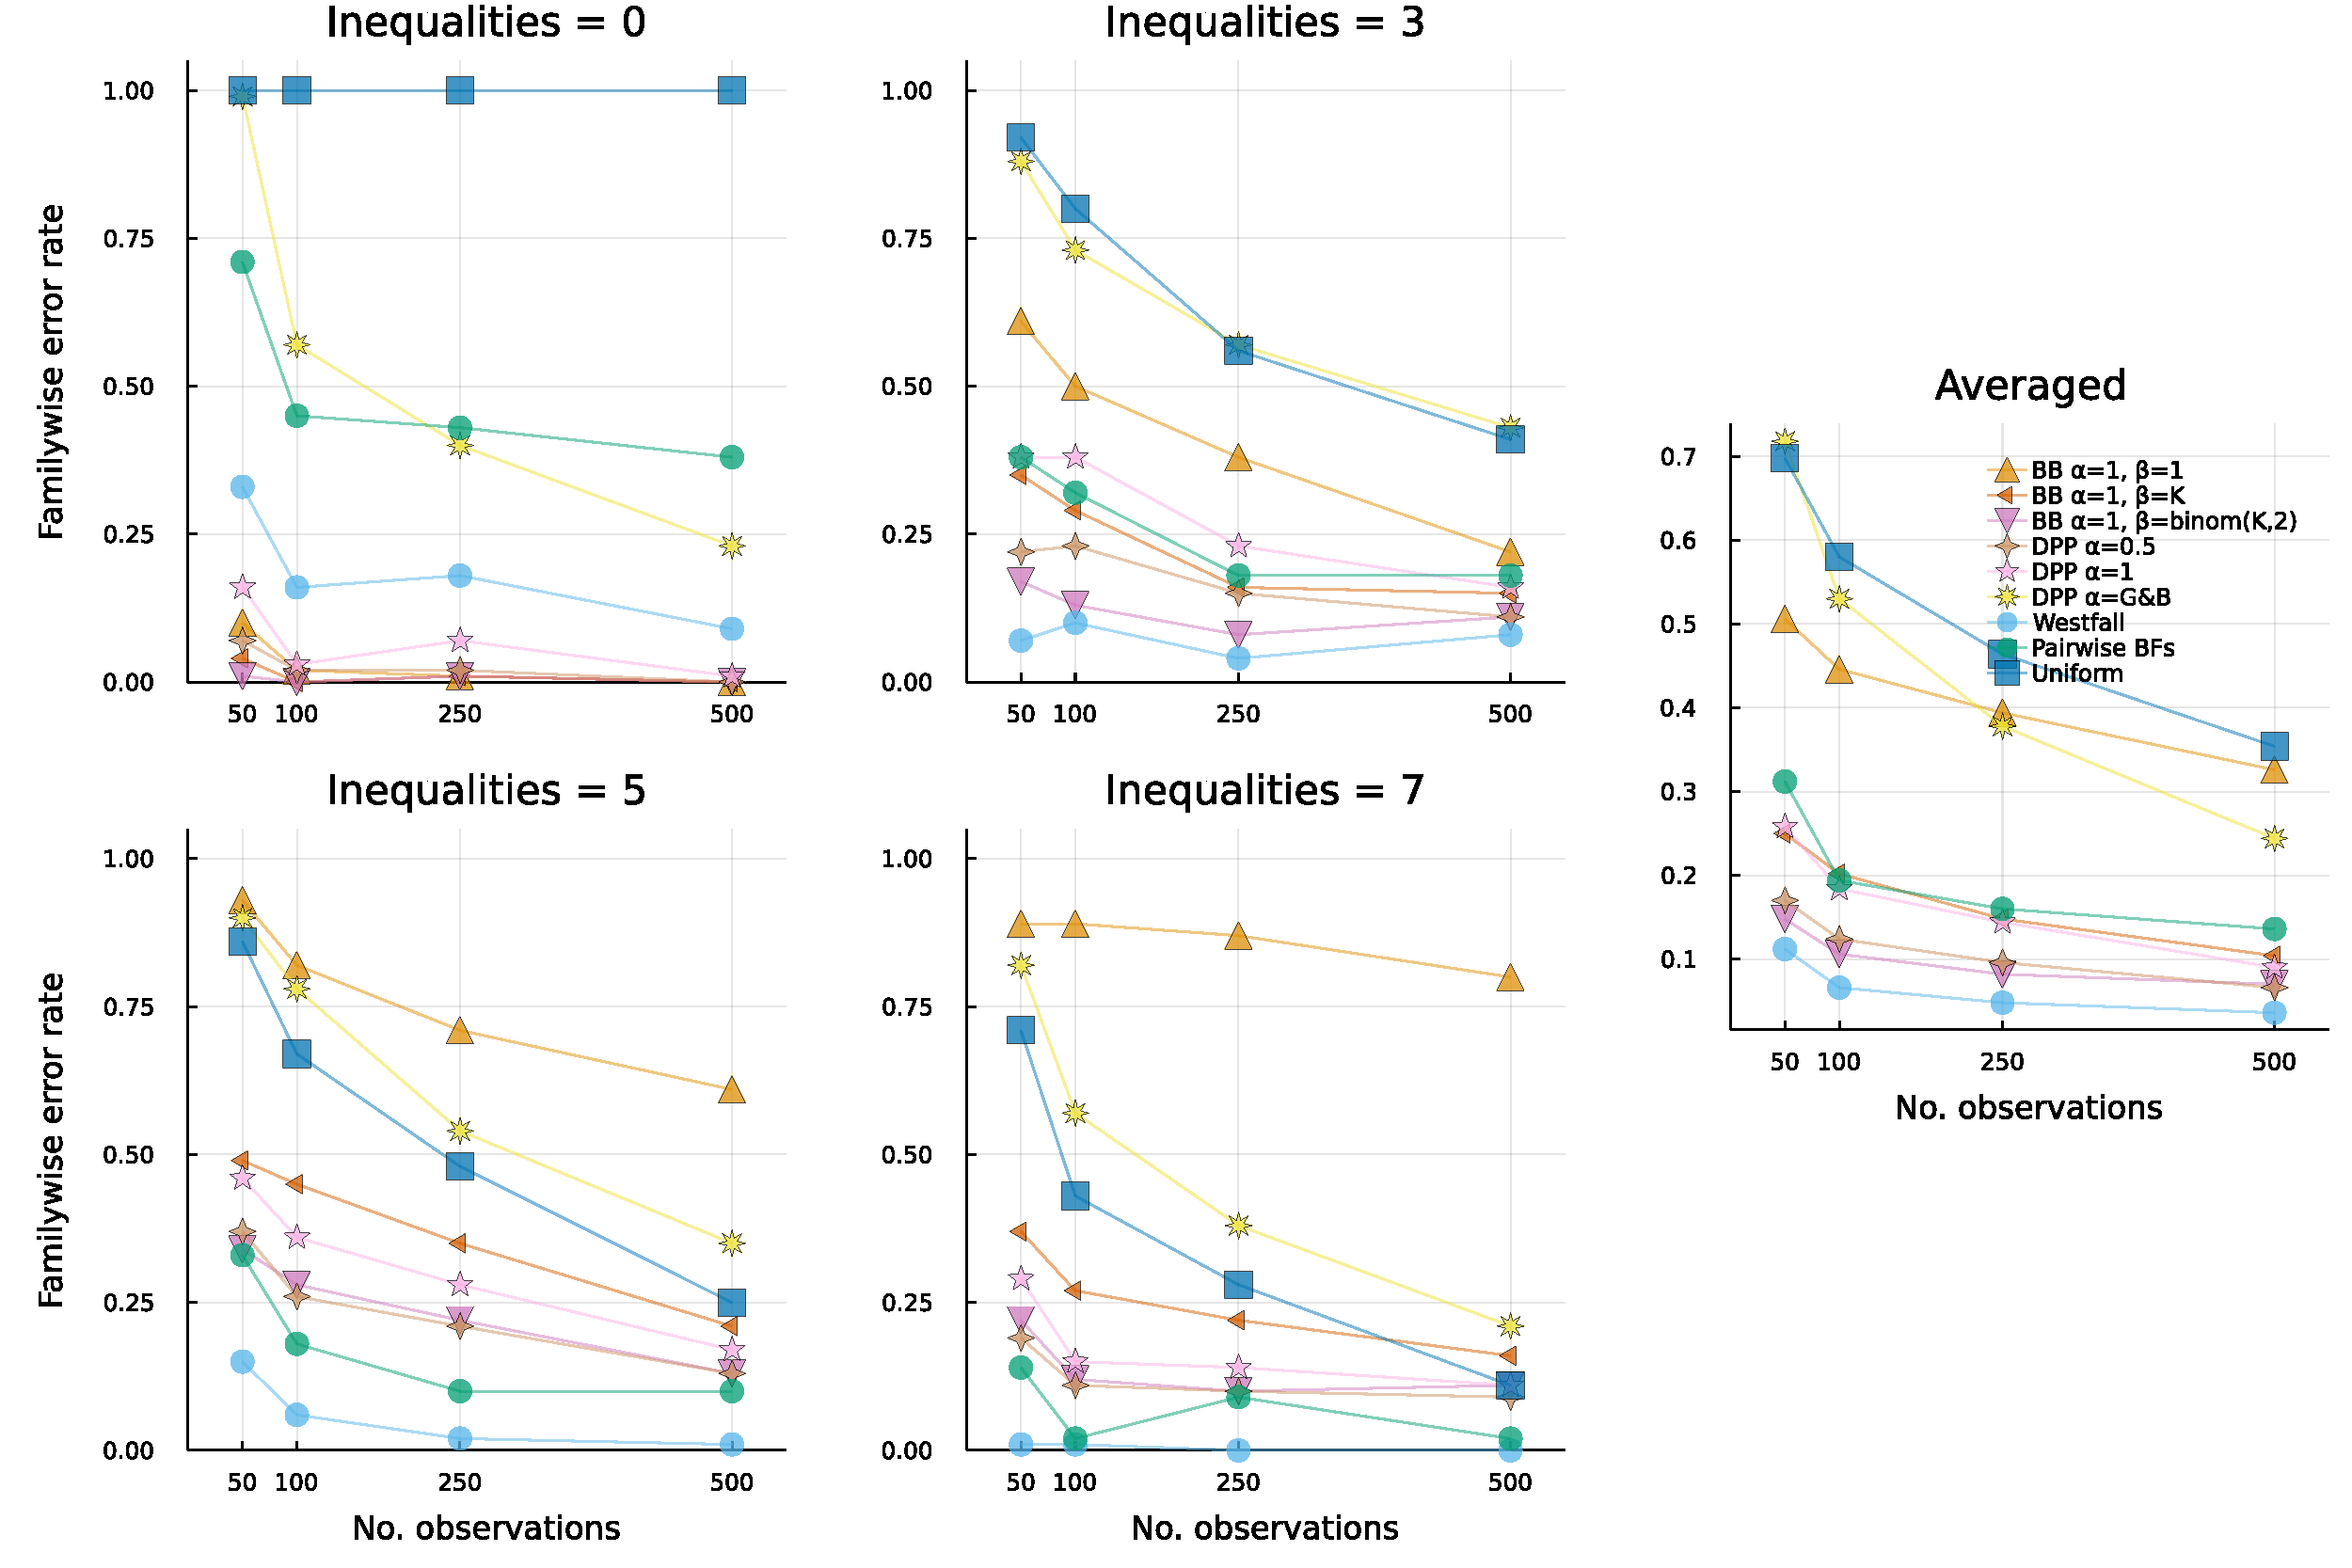
\includegraphics[width=1\textwidth]{subset_k_9_alpha_familywise.pdf}
    \caption{Familywise error rate across priors and sample sizes under a model with 0 (top left), 3 (top right), 5 (bottom left), and 7 (bottom right) true inequalities for $K = 9$ groups. The rightmost panel shows the average familywise error rate across inequalities.}
    \label{fig:big_simulation-k9-I}
\end{figure}

\begin{figure}[!h]
    \centering
    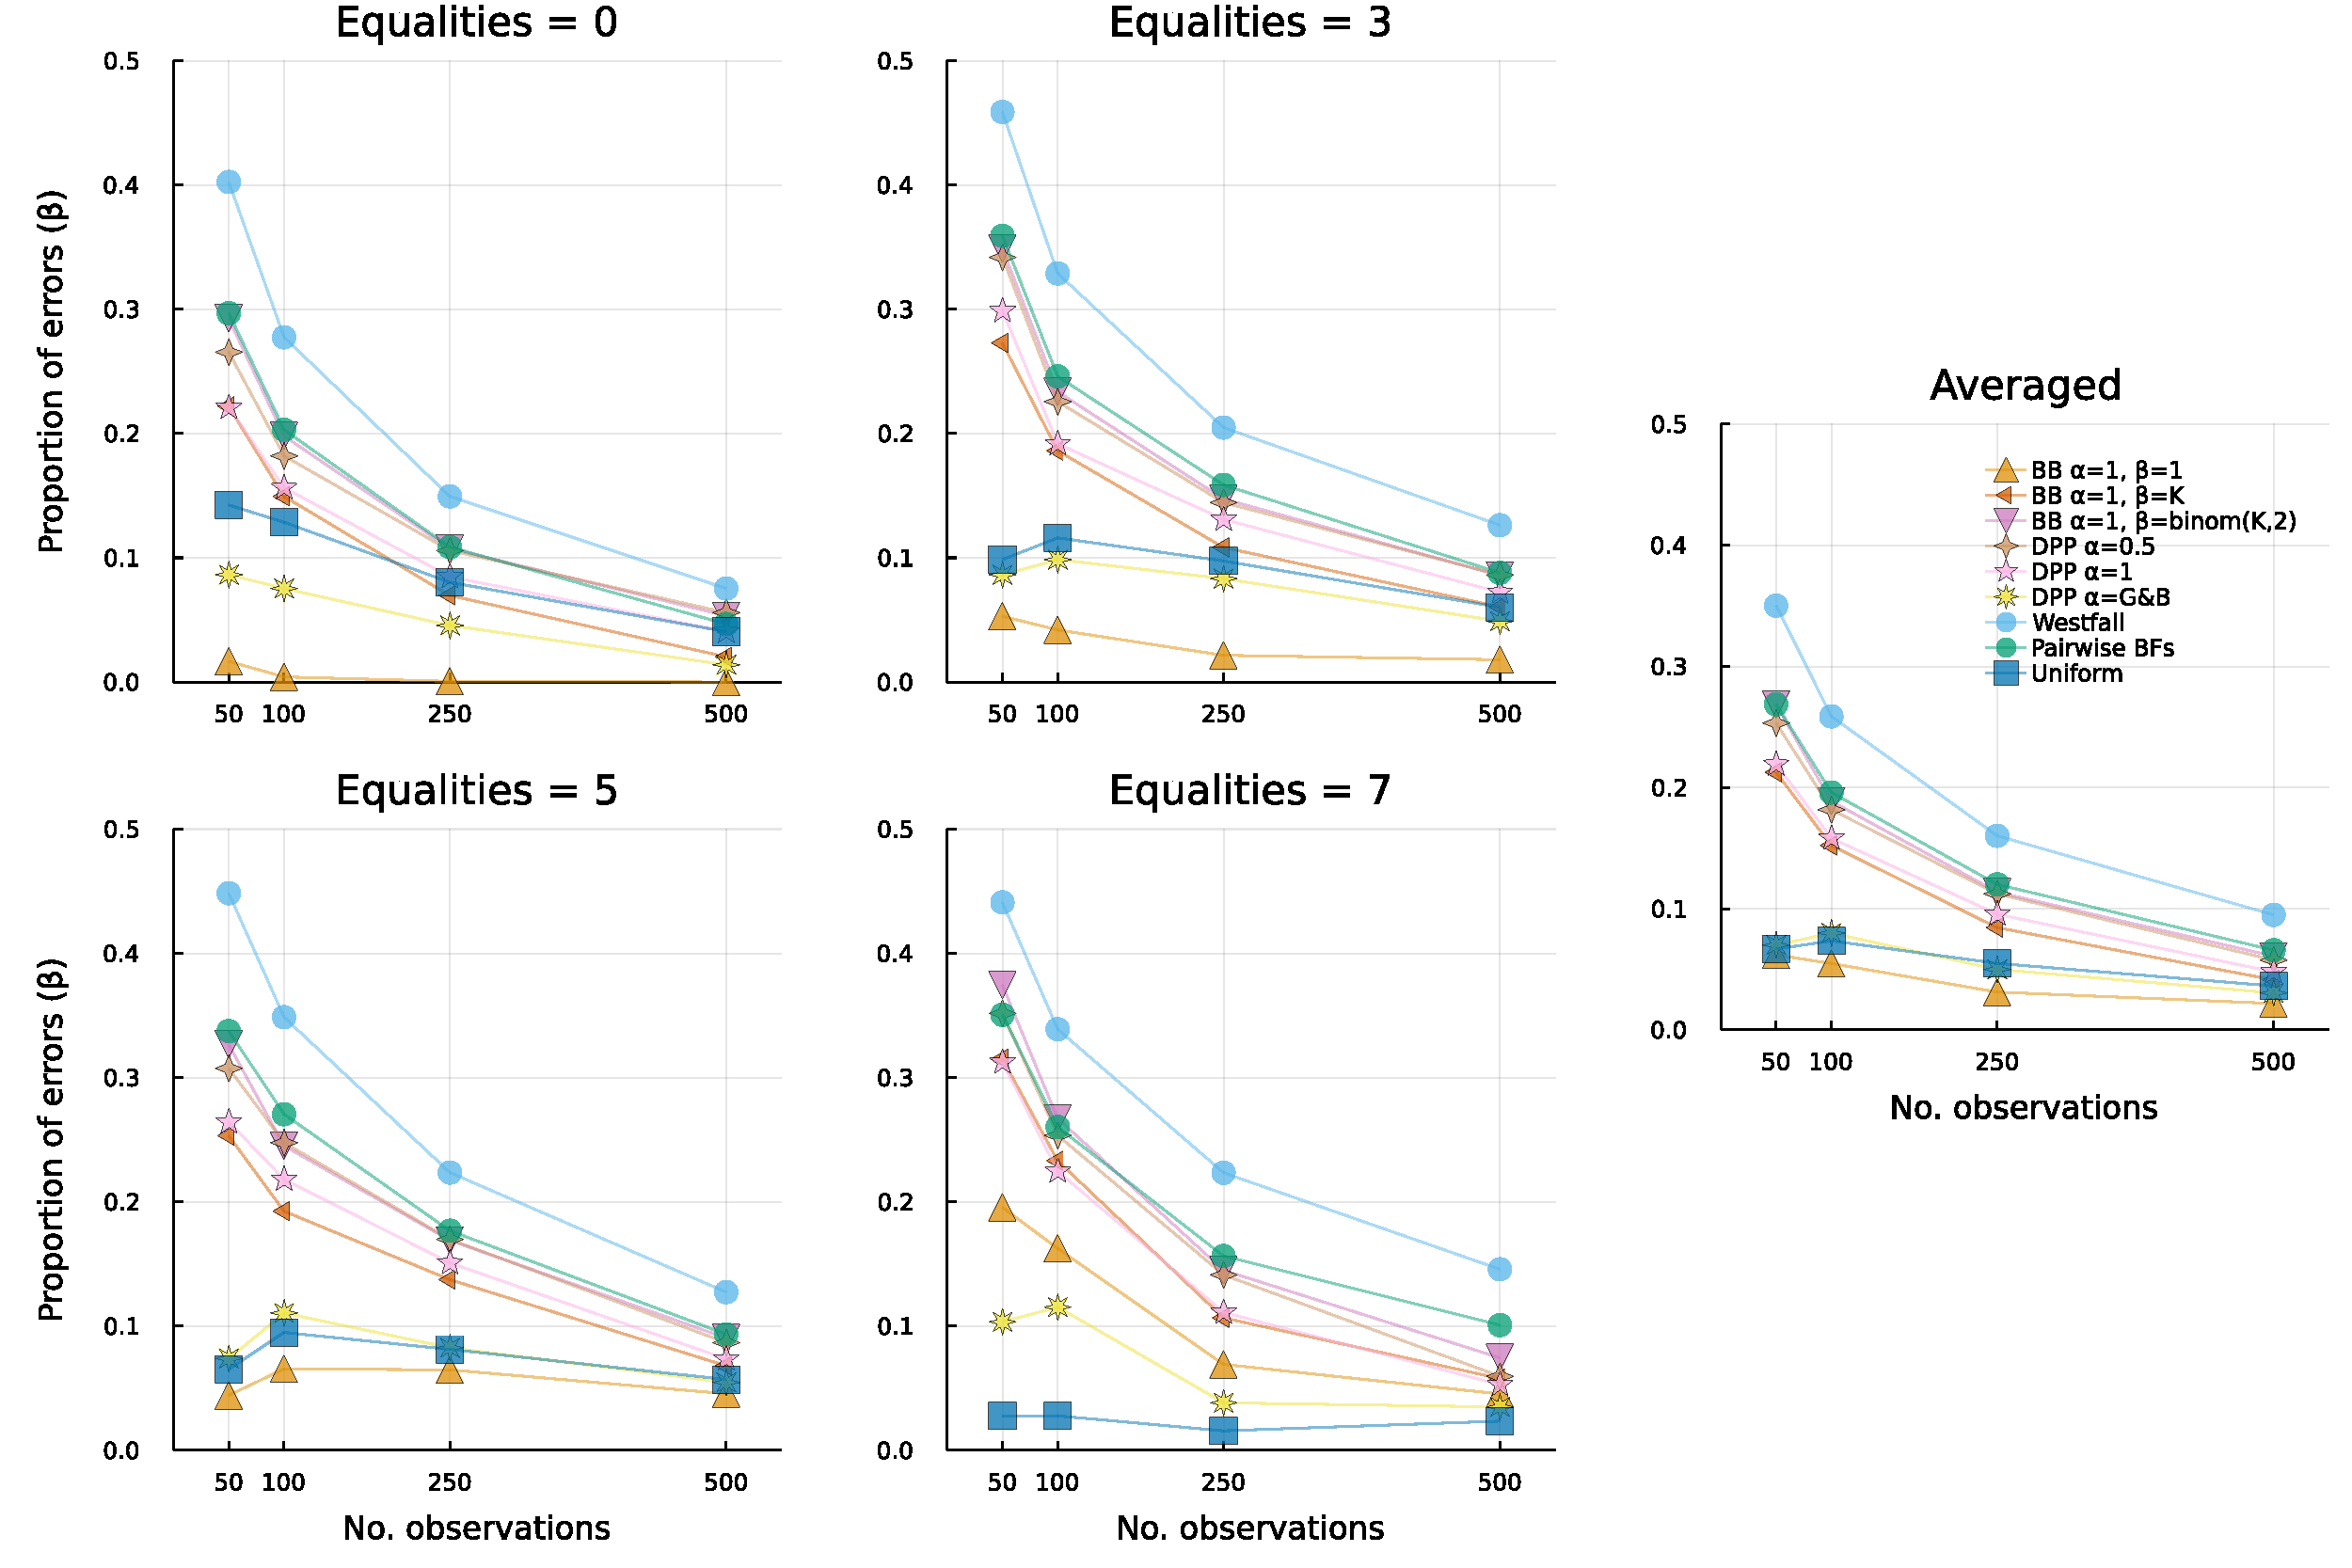
\includegraphics[width=1\textwidth]{subset_k_9_beta.pdf}
    \caption{Proportion of falsely claiming a difference between two groups when there is none across priors and sample sizes under a model with 0 (top left), 3 (top right), 5 (bottom left), and 7 (bottom right) true inequalities for $K = 9$ groups. The rightmost panel shows the average error rate across inequalities.}
    \label{fig:big_simulation-k9-II}
\end{figure}

\iffalse
\section{$\alpha$ and $\beta$ error are complements when summing across partitions} \label{ap:complements}

The proportion of $\alpha$ and $\beta$ errors are defined as $P_\alpha(\rho,\rho^\prime) = \nicefrac{\sum_{1\leq i < j \leq K} I(\rho_i=\rho_j)I(\rho^\prime_i\neq\rho^\prime_j)}{\sum_{1\leq i < j \leq K} I(\rho_i=\rho_j)}$ and $P_\beta(\rho,\rho^\prime) = \nicefrac{\sum_{1\leq i < j \leq K} I(\rho_i\neq\rho_j)I(\rho^\prime_i=\rho^\prime_j)}{ \sum_{1\leq i < j \leq K} I(\rho_i\neq\rho_j)}$ respectively, where $I(\cdot)$ denotes the indicator function, $\rho$ is the `true' partition, and $\rho^\prime$ is the reference partition. In both definitions the numerator counts the number of errors and the denominator counts the number of possible errors given the true partition.
\begin{prop}\label{prop:complements}
The $\alpha$ error proportion averaged across partitions is the complement of the $\beta$ error proportion averaged across partitions, that is,
\begin{align}
    \frac{1}{\bellnum{K}}\sum_{\rho^\prime\in\Rho} P_\alpha(\rho,\rho^\prime) + \frac{1}{\bellnum{K}}\sum_{\rho^\prime\in\Rho} P_\beta(\rho,\rho^\prime) = 1
\end{align}
\end{prop}
\begin{proof}
% Let $C_\alpha(\rho,\rho^\prime) = \sum_{1\leq i < j \leq K} I(\rho_i=\rho_j)I(\rho^\prime_i\neq\rho^\prime_j)$ and $C_\beta(\rho,\rho^\prime) = \sum_{1\leq i < j \leq K} I(\rho_i\neq\rho_j)I(\rho^\prime_i=\rho^\prime_j)$ be two functions that count the number of $\alpha$-errors and $\beta$-errors respectively, where $I(\cdot)$ denotes the indicator function, $\rho$ is the `true' partition, and $\rho^\prime$ is the reference partition. Note that $C_\beta(\rho,\rho^\prime) = C_\alpha(\rho^\prime, \rho)$.

% The total number of possible $\alpha$ and $\beta$ errors for a true partition are given by $T_\alpha(\rho) = \sum_{1\leq i < j \leq K} I(\rho_i=\rho_j)$ and $T_\beta(\rho) = \sum_{1\leq i < j \leq K} I(\rho_i\neq\rho_j)$. Note that $T_\beta(\rho) = \binom{K}{2} - T_\alpha(\rho)$.

% The proportion of $\alpha$ and $\beta$ errors is given by $P_\alpha(\rho,\rho^\prime) = C_\alpha(\rho,\rho^\prime) / T_\alpha(\rho,\rho^\prime)$ and $P_\beta(\rho,\rho^\prime) = C_\beta(\rho,\rho^\prime) / T_\beta(\rho,\rho^\prime)$ respectively.

% We now consider the sums:
% \begin{align}
%     \sum_{\rho^\prime\in\Rho} P_\alpha(\rho,\rho^\prime),\text{ and }
%     \sum_{\rho^\prime\in\Rho} P_\beta(\rho,\rho^\prime).
% \end{align}
% Expanding yields
% \begin{align}
%     \sum_{\rho^\prime\in\Rho} P_\alpha(\rho,\rho^\prime)
%     =&\frac{1}{T_\alpha(\rho)}\sum_{\rho^\prime\in\Rho} \sum_{1\leq i < j \leq K} I(\rho_i=\rho_j)I(\rho^\prime_i\neq\rho^\prime_j)\\
%     \intertext{interchange the sums and observe that $I(\rho_i=\rho_j)$ can be factored out}
%     =&\frac{1}{T_\alpha(\rho)} \sum_{1\leq i < j \leq K} I(\rho_i=\rho_j)\sum_{\rho^\prime\in\Rho}I(\rho^\prime_i\neq\rho^\prime_j)\\
%     \intertext{Note that $\sum_{\rho^\prime\in\Rho}I(\rho^\prime_i\neq\rho^\prime_j) = \sum_{l=1}^{K-1}l\stirling{K-1}{l}$ and is independent of $i$ and $j$. % see https://oeis.org/A005493
%     We obtain}
%     =&\frac{1}{T_\alpha(\rho)} \sum_{1\leq i < j \leq K} I(\rho_i=\rho_j)\sum_{l=1}^{K-1}l\stirling{K-1}{l}\\
%     \intertext{Rearranging yields}
%     =&\left(\sum_{l=1}^{K-1}l\stirling{K-1}{l}\right)\frac{\sum_{1\leq i < j \leq K} I(\rho_i=\rho_j)}{T_\alpha(\rho)}
% \intertext{Notice that the numerator in the fraction is the definition of $T_\alpha(\rho)$ and therefore we have}
%     \sum_{\rho^\prime\in\Rho} P_\alpha(\rho,\rho^\prime)
%     =& \sum_{l=1}^{K-1}l\stirling{K-1}{l}= \bellnum{K} - \bellnum{K-1}
% \end{align}
% $\sum_{\rho^\prime\in\Rho} P_\beta(\rho,\rho^\prime)$ simplifies in a similar manner except that $\sum_{\rho^\prime\in\Rho}I(\rho^\prime_i=\rho^\prime_j) = \bellnum{K-1}$ which yields
% \begin{align}
%     \sum_{\rho^\prime\in\Rho} P_\beta(\rho,\rho^\prime)
%     =&\bellnum{K-1}
% \end{align}
% Note that $\sum_{\rho^\prime\in\Rho} P_\alpha(\rho,\rho^\prime) + \sum_{\rho^\prime\in\Rho} P_\beta(\rho,\rho^\prime) = \bellnum{K}$.
% Since we average the error across partitions rather than summing, we have $\frac{1}{\bellnum{K}}\sum_{\rho^\prime\in\Rho} P_\alpha(\rho,\rho^\prime) + \frac{1}{\bellnum{K}}\sum_{\rho^\prime\in\Rho} P_\beta(\rho,\rho^\prime) = 1$.

Consider the sums:
\begin{align}
    \sum_{\rho^\prime\in\Rho} P_\alpha(\rho,\rho^\prime),\text{ and }
    \sum_{\rho^\prime\in\Rho} P_\beta(\rho,\rho^\prime).
\end{align}
Expanding yields
\begin{align}
    \sum_{\rho^\prime\in\Rho} P_\alpha(\rho,\rho^\prime)
    =&\frac{1}{\sum_{1\leq i < j \leq K} I(\rho_i=\rho_j)}\sum_{\rho^\prime\in\Rho} \sum_{1\leq i < j \leq K} I(\rho_i=\rho_j)I(\rho^\prime_i\neq\rho^\prime_j)\\
    \intertext{interchange the sums and observe that $I(\rho_i=\rho_j)$ can be factored out}
    =&\frac{1}{\sum_{1\leq i < j \leq K} I(\rho_i=\rho_j)} \sum_{1\leq i < j \leq K} I(\rho_i=\rho_j)\sum_{\rho^\prime\in\Rho}I(\rho^\prime_i\neq\rho^\prime_j)\\
    \intertext{Note that $\sum_{\rho^\prime\in\Rho}I(\rho^\prime_i\neq\rho^\prime_j) = \sum_{l=1}^{K-1}l\stirling{K-1}{l}= \bellnum{K} - \bellnum{K-1}$ and is independent of $i$ and $j$. % see https://oeis.org/A005493
    We obtain}
    =&\frac{1}{\sum_{1\leq i < j \leq K} I(\rho_i=\rho_j)} \sum_{1\leq i < j \leq K} I(\rho_i=\rho_j)
    \left(\bellnum{K} - \bellnum{K-1}\right)\\
    =&\left(\bellnum{K} - \bellnum{K-1}\right)\frac{\sum_{1\leq i < j \leq K} I(\rho_i=\rho_j)}{\sum_{1\leq i < j \leq K} I(\rho_i=\rho_j)}\\
    =& \bellnum{K} - \bellnum{K-1}.
\end{align}
$\sum_{\rho^\prime\in\Rho} P_\beta(\rho,\rho^\prime)$ simplifies in a similar manner except that $\sum_{\rho^\prime\in\Rho}I(\rho^\prime_i=\rho^\prime_j) = \bellnum{K-1}$ and so $\sum_{\rho^\prime\in\Rho} P_\beta(\rho,\rho^\prime) =\bellnum{K-1}$.

It follows that $\sum_{\rho^\prime\in\Rho} P_\alpha(\rho,\rho^\prime) + \sum_{\rho^\prime\in\Rho} P_\beta(\rho,\rho^\prime) = \bellnum{K}$.
Since we average across partitions rather than summing, we obtain $\frac{1}{\bellnum{K}}\sum_{\rho^\prime\in\Rho} P_\alpha(\rho,\rho^\prime) + \frac{1}{\bellnum{K}}\sum_{\rho^\prime\in\Rho} P_\beta(\rho,\rho^\prime) = 1$.

\end{proof}
\fi

\end{document}
